\documentclass[10pt]{article}
\usepackage{c2f}
\usepackage{tabularx}
\usepackage{placeins}
\usepackage{needspace}
\usepackage{url}
% ---------- notation ----------
\newcommand{\method}{\textup{\textsc{TWoS}}}
\newcommand{\R}{\mathbb{R}}
\newcommand{\E}{\mathbb{E}}
\newcommand{\Prob}{\mathbb{P}}
\newcommand{\Var}{\operatorname{Var}}
\newcommand{\Cov}{\operatorname{Cov}}
\newcommand{\J}{\mathcal{J}}
\newcommand{\DT}{D_{\!T}}
\newcommand{\eps}{\varepsilon}
\newcommand{\ind}{\mathbb{1}}
\newcommand{\norm}[1]{\left\lVert #1\right\rVert}
\newcommand{\abs}[1]{\left\lvert #1\right\rvert}

\setlength{\emergencystretch}{3em}
% the appendix carries many full-width figures: let them share pages and stay near their sections
\setcounter{topnumber}{3}\setcounter{bottomnumber}{2}\setcounter{totalnumber}{4}
\renewcommand{\topfraction}{0.9}\renewcommand{\bottomfraction}{0.6}
\renewcommand{\textfraction}{0.08}\renewcommand{\floatpagefraction}{0.75}

\hypersetup{pdftitle={Walking into Holes: Monte Carlo Topological Derivatives for Grid-Free PDE-Constrained Design},pdfauthor={Johannes Herter}}

\PaperTitle{Walking into Holes: Monte Carlo Topological Derivatives\\[2pt] for Grid-Free PDE-Constrained Design}
\PaperAuthors{Johannes Herter}
\PaperAffiliations{ETH Z\"urich}
\PaperAbstract{%
Creating a new interior boundary requires a different design decision from moving an existing surface. We address cavity nucleation using ideal cooled cavities in heat-generating solids. Classical topological derivatives express insertion benefit through state and adjoint fields. Topological Walk on Spheres (\method{}) estimates this coefficient with local random walks on the current geometry, without a volumetric PDE discretization or a shrinking trial hole. Cross-index products remove primal--adjoint correlation bias under explicit independence assumptions. We derive radius-independent variance and conditions for finite-insertion error control, including oracle bias, asymptotic error, and adaptive selection. A separate variational bound certifies finite Poisson-compliance benefit under stated sampling and geometry assumptions. Experiments compare actual-mesh estimators, complete insertion--refinement pipelines, and accessible channels with fixed material and heat-input budgets. Uncertainty bands and independent numerical checks retain competitive multigrid and proximity controls. Matched-accuracy query sweeps expose strong dependence on source, objective, and field reuse; fresh-seed checks qualify apparent sparse-query gains. Conditional validation has substantial additional cost.}

\begin{document}
\MakeTitleBox
\suppressfloats[t]

\begin{figure}[t]
  \centering
  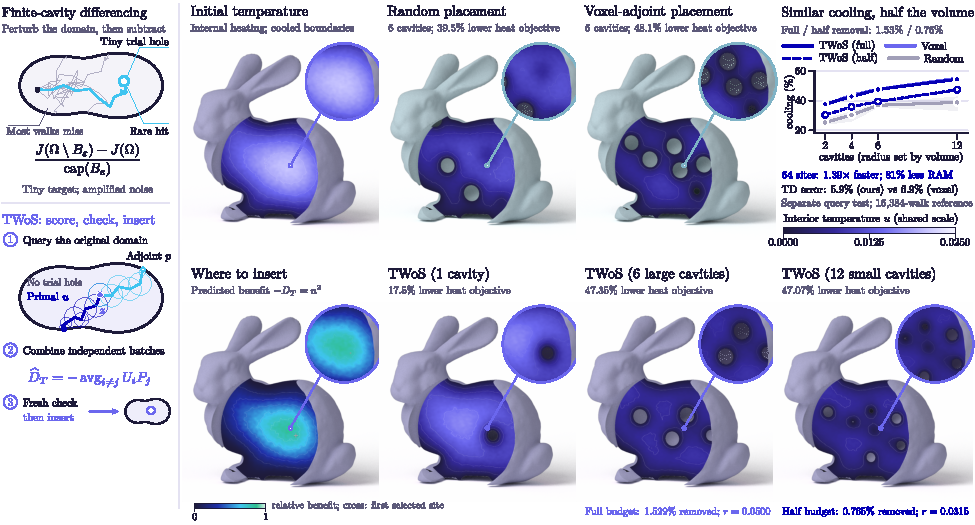
\includegraphics[width=\textwidth]{figures/mesh-hero.pdf}
  \caption{\textbf{Choosing where new cooled cavities should appear.} \method{} queries the current geometry to estimate insertion benefit, then adds selected cavities. Top: initial temperature and six-cavity random and voxel-adjoint designs. Bottom: the initial benefit field, an illustrative first insertion, and two \method{} allocations with similar measured cooling: six large cavities versus twelve small cavities at half the removed volume. These cavities have ideal zero-temperature walls. Temperature views share one color scale; benefit has a separate scale. The cut and inset edges are for display only, and some cavities lie outside the section. Per-design labels use independent objective evaluations; the plot summarizes three design seeds. The speed and memory callouts describe a separate 64-site query benchmark, not the full Bunny optimization. Field rendering and evaluation protocols appear in \cref{sec:bunnybudget,app:renderprotocol}.}
  \label{fig:teaser}
\end{figure}


\section{Introduction}
\label{sec:introduction}

Computational design chooses geometry to produce a desired physical response.
Changing an existing boundary and deciding where a new boundary should appear
are different decisions. We study the latter: selecting interior cavities in
a solid to improve a PDE-defined objective. In our thermal application,
prescribed cold cavity walls act as ideal internal heat sinks. Their placement
changes conduction paths and the temperature of protected components. This
model isolates a geometry-design problem; it does not simulate coolant flow.

A candidate could be scored by inserting a small trial hole, solving the
modified PDE, and subtracting objectives. Classical topological derivatives
avoid these repeated trial solves by expressing the leading change through
the current state and adjoint~\cite{cea2000topological,novotny2012topological}.
Global discretized solvers already exploit this formula. We ask how to evaluate
it directly using local random walks on the boundary representation, without
constructing a volumetric PDE discretization or a trial cavity.

Walk on Spheres and Walk on Stars provide the necessary point-query
machinery~\cite{muller1956some,sawhney2023walk}. Differential WoS supplies
sensitivities for existing geometry~\cite{miller2024differential}.
Our additional query is the capacity-normalized response to creating an
interior boundary. We call its direct estimator \emph{Topological Walk on
Spheres} (\method{}). Primal and adjoint estimates can share a walk skeleton;
cross-index products remove the resulting correlation bias when complete
oracle pairs are independent. The estimator has no trial-radius parameter.

The problem is therefore a missing query in the grid-free design workflow:
\emph{where would a new boundary help?} Our contribution is the stochastic
evaluation and deployment of classical topological sensitivity. The deterministic derivative, cross-index unbiasedness, and the
Hoeffding decomposition are classical ingredients. The technical question
is how their
combination supports an insertion query and which additional assumptions
turn that query into a finite geometric decision. We give the exact product-estimator variance,
identify a shrinking-target variance barrier for specified finite-cavity
couplings, and propagate sampling error, oracle bias, finite-radius error,
and adaptive selection into explicit decision conditions. A separate
variational argument gives a finite-benefit bound for Poisson compliance
without an unknown asymptotic remainder. The appendix contains every
derivation and the additional assumptions needed by implementations.

The experiments distinguish placement quality from numerical performance.
Three different solids compare complete cavity-initialization and Differential
WoS refinement pipelines against tuned multigrid and geometric proximity.
Matched-volume channels preserve the entire heat input. Actual-mesh estimator
tests complement controlled statistical diagnostics, and a detailed Bunny
study measures the crossover from sparse queries to a global solve.
The evidence supports direct stochastic insertion scores; it also retains
competitive deterministic and proximity controls rather than claiming
universal design or runtime superiority.

\section{Related Work}
\label{sec:related}

\paragraph{Grid-free PDE evaluation and differentiation.}
WoS estimates Dirichlet solutions using sphere exits~\cite{muller1956some}; WoSt extends the approach to mixed boundaries~\cite{sawhney2023walk}, with related estimators for Robin conditions~\cite{miller2024robin}. Differential WoS computes sensitivities to problem parameters and geometry through point queries~\cite{miller2024differential}, and derivative WoSt improves spatial derivatives near Neumann boundaries~\cite{yu2025robust}. These methods supply the PDE and existing-boundary derivative machinery on which we build. Our additional query is the coefficient of a singular cavity insertion, evaluated before its boundary exists. Fast cage cutting instead updates solutions after an explicit edit~\cite{saeed2026fast}. Flexible boundary representations and efficient updates are complementary to selecting where a new feature should be introduced.

\paragraph{Probabilistic shape optimization.}
Schlegel et al.~\cite{schlegel2026probabilistic} derive probabilistic representations of solution and objective shape derivatives for semilinear Dirichlet PDEs. Schmidt and W\"urschmidt~\cite{schmidt2026first} use a probabilistic derivative with a neural state representation to optimize shape. Our target is the capacity-normalized response to nucleating an interior cavity. Such a family is not a regular deformation of the original domain (\cref{prop:notshapepath}), although topological derivatives can be related to singular limits of shape derivatives on already perforated domains. We retain this established distinction without attributing topology-preservation limitations to every possible implementation of shape optimization.

\paragraph{Topological sensitivity and inverse design.}
Small-feature asymptotics and state--adjoint formulas are standard tools in topology optimization~\cite{cea2000topological,novotny2012topological,baumann2022complete,gangl2022automated}. They complement level-set boundary evolution~\cite{allaire2004structural,burger2004incorporating}; recent developments address finite-element recovery~\cite{li2026superconvergence}. Meshfree spline methods already optimize holes using topological derivatives~\cite{hur2017topology}, and immersed isogeometric methods avoid remeshing using background spline spaces~\cite{teixeira2026isogeometric}. Neural implicit material representations offer another design parameterization~\cite{zehnder2021ntopo}. In graphics, Mehta et al.~\cite{mehta2023theory} derive topological derivatives for inverse rendering. Our deterministic coefficient builds on this calculus; the focus is its direct random-walk evaluation and the resulting uncertainty in geometric decisions. Freiberger et al.~\cite{freiberger2011using} use a deterministically computed topological derivative to initialize MCMC reconstruction, a different role for Monte Carlo from estimating the derivative itself.

\paragraph{Sampling efficiency and operator scope.}
Boundary-value, harmonic, and probe caches amortize spatial queries~\cite{miller2023boundary,zhou2025harmonic,huang2026probe}; neighbor reuse shares completed walks~\cite{czekanski2026neighbors}. RQMC and Array-RQMC reduce sampling error~\cite{ho2026randomized,ho2026array}. We examine these accelerations through an independent-randomization interface: dependent paths within one array or cache are not independent observations for cross-fitting. Learned correction introduces a separate bias--variance tradeoff~\cite{hsu2026mc2}. Volumetric WoS, extended elliptic solvers, and transient diffusion broaden the PDE toolkit~\cite{miller2025volumetric,cimpean2026extended,zhou2026transient}; transferring cavity derivatives to those models requires the corresponding analysis.

\paragraph{Connectivity constraints.}
Andrade et al.~\cite{andrade2026connectivity} combine topological sensitivity with a spectral constraint on void connectivity. Their exterior-Dirichlet construction addresses whether void regions reach the exterior. Our strictly overlapping ball union guarantees an internally connected cavity, whose terminals remain inside the object. These are different feasible sets. The reproduced spectral diagnostic in \cref{sec:critical} clarifies the distinction; it is not a matched comparison of complete connectivity optimizers.

\section{Problem and Topological Expansion}
\label{sec:problem}

\paragraph{Design task.}
Given an outer solid, a heat source, boundary data, and geometric constraints, we select interior cavity locations to reduce a PDE-defined objective. The thermal experiments solve $-\Delta u=f$ with $u=0$ on the exterior and cavity walls. Compliance $J=\int fu$ rewards cooling where heat is generated. A common fixed original-domain normalization is used when reporting its Monte Carlo objective averages, with zero contribution from removed material. For this objective, the adjoint source equals the state source; together with the self-adjoint operator, this gives $p=u$ and normalized insertion benefit $-D_T=u^2$. Self-adjointness of the operator alone does not imply $p=u$: the regional objective $J_q=\int qu/\int q$ instead uses a distinct adjoint driven by $q$, as evaluated in \cref{sec:regional}. The cavity walls are ideal heat sinks; cooling access and coolant transport are outside this model.

The analysis below treats the broader scalar, self-adjoint screened Poisson setting. Its regularity and oracle assumptions state the scope of the theorems; the 3D implementation specializes to constant conductivity and zero screening. Detailed proofs appear in \cref{app:deterministic}.

\subsection{State, adjoint, and reduced objective}

Let $\Omega\subset\R^d$, $d\in\{2,3\}$, be bounded and connected.  Its fixed
outer boundary is partitioned into a relatively open Dirichlet part
$\Gamma_D$ and a Neumann part $\Gamma_N$, with
$\mathcal H^{d-1}(\Gamma_D)>0$.  Define
\begin{equation}
 V:=H^1_{\Gamma_D}(\Omega)
 :=\{v\in H^1(\Omega):\operatorname{Tr}v=0
       \text{ on }\Gamma_D\}
\end{equation}
and, for every measurable $D\subseteq\Omega$,
\begin{equation}
 a_D(v,w):=\int_D
 \kappa\,\nabla v\!\cdot\!\nabla w+\sigma vw\,\mathrm dx.
 \label{eq:bilinear}
\end{equation}
The state $u\in g+V$ is the unique solution of
\begin{equation}
 a_\Omega(u,v)=\ell_\Omega(v)
 \qquad\forall v\in V,
 \label{eq:stateweak}
\end{equation}
where $g$ is a fixed Dirichlet lift and $\ell_\Omega\in V^*$ contains the
volume source and prescribed Neumann data.  In strong form this is
$-\nabla\!\cdot(\kappa\nabla u)+\sigma u=f$.

Let $j:L^2(\Omega)\to\R$ be the state-dependent objective and let
$\psi\in L^\infty(\Omega)$ be an optional explicit domain cost.  We set
\begin{equation}
 \J(\Omega):=j(u)+\int_\Omega\psi(x)\,\mathrm dx.
 \label{eq:baseobjective}
\end{equation}
The adjoint $p\in V$ is defined by
\begin{equation}
 a_\Omega(v,p)=j'(u)[v]
 \qquad\forall v\in V.
 \label{eq:adjointweak}
\end{equation}
For example, if
$j(u)=\tfrac12\int_\Omega w(x)(u-u_\star)^2\,\mathrm dx$ with bounded
$w\ge0$, then the adjoint source is $w(u-u_\star)$.

\subsection{A finite Dirichlet cavity}

Let $B\subset\R^d$ be a fixed bounded inclusion containing the origin.  For a
candidate $z$ and scale $\eps>0$, put
\begin{equation}
 K_{\eps,z}:=z+\eps B,
 \qquad
 \Omega_{\eps,z}:=\Omega\setminus\overline{K_{\eps,z}}.
\end{equation}
On the new boundary we prescribe the constant value
$u_{\eps,z}=h_z$; in thermal design, $h_z$ is the coolant temperature.  The
perforated state solves the same weak equation on $\Omega_{\eps,z}$, with its
test functions also vanishing on $\partial K_{\eps,z}$.  Extend it to all of
$\Omega$ by the constant $h_z$ inside the cavity and denote this $H^1$
extension by $\widetilde u_{\eps,z}$.  The perturbed reduced objective is
\begin{equation}
 \J(\Omega_{\eps,z})
 :=j(\widetilde u_{\eps,z})
   +\int_{\Omega_{\eps,z}}\psi(x)\,\mathrm dx.
 \label{eq:perforatedobjective}
\end{equation}

The correct normalizer is the \emph{relative operator capacity}.  With
$\widetilde v$ denoting the quasi-continuous representative of $v\in V$, set
\begin{equation}
 \begin{split}
 \rho_z(\eps):=\inf\{a_\Omega(v,v):{}&v\in V,\\[-2pt]
 &\widetilde v\ge1\text{ q.e. on }K_{\eps,z}\}.
 \end{split}
 \label{eq:relativecapacity}
\end{equation}
``Quasi-everywhere'' means outside a set of zero $H^1$ capacity; it is the
trace notion for which \cref{eq:relativecapacity} is closed under weak
convergence.  The infimum is attained by a unique equilibrium potential
$q_{\eps,z}$.  Its leading scale is
\begin{equation}
 \rho_z(\eps)=
 \begin{cases}
  \displaystyle \frac{2\pi\kappa(z)}{|\log\eps|}
       \bigl(1+o(1)\bigr), & d=2,\\[7pt]
  \displaystyle \kappa(z)\operatorname{cap}(B)\eps
       \bigl(1+o(1)\bigr), & d=3,
 \end{cases}
 \label{eq:capacityscaling}
\end{equation}
uniformly on compact candidate sets.  Here $\operatorname{cap}(B)$ is the
Newtonian capacity normalized by the energy $\int_{\R^3}|\nabla v|^2$.

\begin{definition}[Capacity-normalized topological derivative]
The Dirichlet-cavity topological derivative at $z$ is
\begin{equation}
 \DT(z):=\lim_{\eps\downarrow0}
 \frac{\J(\Omega_{\eps,z})-\J(\Omega)}{\rho_z(\eps)},
 \label{eq:tddefinition}
\end{equation}
whenever the limit exists.
\end{definition}

\begin{assumption}[Analytic setting]
\label{ass:regularity}
$\Omega$ and $B$ are $C^{2,\alpha}$ domains for some $\alpha\in(0,1)$;
$0\in\operatorname{int}B$; the mixed-boundary decomposition admits the
Poincar\'e inequality, maximum principle, and Green kernel used in
\cref{app:deterministic};
$\kappa\in C^{1,\alpha}(\overline\Omega)$ satisfies
$0<\kappa_-\le\kappa\le\kappa_+$; and
$\sigma\in L^\infty(\Omega)$ is nonnegative.  Candidates lie in a compact
$Z\Subset\Omega$, and $u,p\in C^{1,\alpha}(U)$ on a fixed neighborhood
$U\Supset Z$.  The values $h_z$ are uniformly bounded on $Z$.
\end{assumption}

\begin{assumption}[Objective smoothness]
\label{ass:objective}
$j$ is twice Fr\'echet differentiable on an $L^2(\Omega)$ neighborhood of
$u$, with $\|j''(v)\|$ uniformly bounded there, and
$\psi\in L^\infty(\Omega)$.  The load restricted to a perforated domain is
the restriction of the unperforated load, so state differences are
$a$-harmonic away from the cavity.
\end{assumption}

\begin{theorem}[Relative-capacity asymptotics]
\label{thm:capacityscale}
Under \cref{ass:regularity}, the minimizer in
\cref{eq:relativecapacity} exists, is unique, and satisfies
\cref{eq:capacityscaling}.  Moreover, $\rho_z(\eps)>0$ and
$\eps^d=o(\rho_z(\eps))$ uniformly for $z\in Z$.
\end{theorem}

\begin{theorem}[Quantitative local topological expansion]
\label{thm:localtd}
Under \cref{ass:regularity,ass:objective}, there are constants
$C>0$ and $\eps_0>0$, independent of $z\in Z$, such that for
$0<\eps\le\eps_0$,
\begin{equation}
 \left|\J(\Omega_{\eps,z})-\J(\Omega)
 -\rho_z(\eps)\DT(z)\right|
 \le C\rho_z(\eps)^{1+\alpha_d},
 \label{eq:quantitativesmallhole}
\end{equation}
where $\alpha_2=1$ and $\alpha_3=\tfrac12$, and
\begin{equation}
 \boxed{\DT(z)=-\bigl(u(z)-h_z\bigr)p(z).}
 \label{eq:localproduct}
\end{equation}
In particular, the limit in \cref{eq:tddefinition} exists uniformly on $Z$.
\end{theorem}

The proof in \cref{app:deterministic} constructs the equilibrium measure,
proves its concentration on the shrinking cavity, obtains the full state
corrector by an energy-minimizing lift, controls the nonlinear objective
remainder in $L^2$, and only then invokes the adjoint identity.  Thus the sign
in \cref{eq:localproduct} follows from the convention in
\cref{eq:adjointweak}; changing that convention changes the displayed sign,
not the algorithm.

\begin{remark}[Why regular shape calculus is insufficient]
For $d=3$, the objective change is $O(\eps)$ even though the new boundary area
is $O(\eps^2)$; in $d=2$ it is $O(1/|\log\eps|)$.  Differentiating with
respect to $\eps$ and then setting $\eps=0$ therefore does not recover a
regular shape derivative.  Capacity normalization is the essential singular
step.
\end{remark}



For connected outer and cavity boundaries, \cref{prop:notshapepath} makes
this distinction explicit: a diffeomorphism preserves boundary connectedness,
whereas an interior cavity creates a second boundary component.
This elementary observation does not exclude recovering a topological
derivative through a singular limit of shape derivatives on already
perforated domains.  Such connections are established prior
art~\cite{cea2000topological}; the proposition makes no novelty claim about
the distinction itself.

\section{Topological Walk on Spheres}
\label{sec:method}

Equation~\eqref{eq:localproduct} turns a domain-perturbation limit into two point queries on the original domain.  This section constructs an estimator that remains correct under the correlated reuse patterns needed in a fast implementation.

\subsection{Primal and adjoint random-walk oracles}

At candidate $z$, let a WoS/WoSt implementation return a random pair
\begin{equation}
  X_i(z):=(U_i(z),P_i(z)), \qquad i=1,\dots,N,
\end{equation}
where pairs are independent and identically distributed across $i$, but $U_i$ and $P_i$ may share a seed, geometric queries, path prefixes, or a harmonic cache.  We first analyze exact oracles,
\begin{equation}
  \E[U_i(z)]=u(z),\qquad \E[P_i(z)]=p(z),
  \label{eq:oraclemeans}
\end{equation}
and later place termination and cache error into an explicit bias budget.  Screened Poisson killing, source sampling, Walk on Stars, and variance reduction can all live behind this interface.

\paragraph{The independence unit is an entire randomization.}
For Array-RQMC or a randomly constructed cache shared across many trajectories,
individual paths are not independent oracle pairs.  Instead, generate $R\ge2$
independent complete randomizations and use their field averages
$X_r=(\bar U_r,\bar P_r)$ in \cref{eq:ustatpairwise}, with $N=R$.
Within a randomization, primal and adjoint may reuse every trajectory; neighbor
queries may also share all cached paths.  Different randomizations must use
independent random streams and independently generated random caches.
The finite-sample radius then uses $\lfloor R/2\rfloor$, not the number of
paths or cross-products.  This interface preserves compatibility with
Array-RQMC~\cite{ho2026array} and neighbor reuse~\cite{czekanski2026neighbors}
without importing an independence assumption they do not satisfy.
The exact bias identities and a counterexample appear in
\cref{app:batchindependence}.

The source-integral identity used by our three-dimensional Poisson implementation is stated and proved in \cref{prop:greenballsample}. General objectives require a valid adjoint oracle as well as a state oracle; the product construction does not by itself solve the adjoint PDE or remove bias from a learned or approximate adjoint source. Compliance experiments exploit $p=u$; sensor-protection experiments solve the distinct adjoint driven by the observation weight.

A naive product from a same-seed pair is biased whenever $U_i$ and $P_i$ are correlated; its bias is $-\Cov(U_i,P_i)$.  Independently generating every primal and adjoint path avoids that covariance but forfeits useful reuse.  We instead remove all same-index products.

\begin{figure}[t]
 \centering
 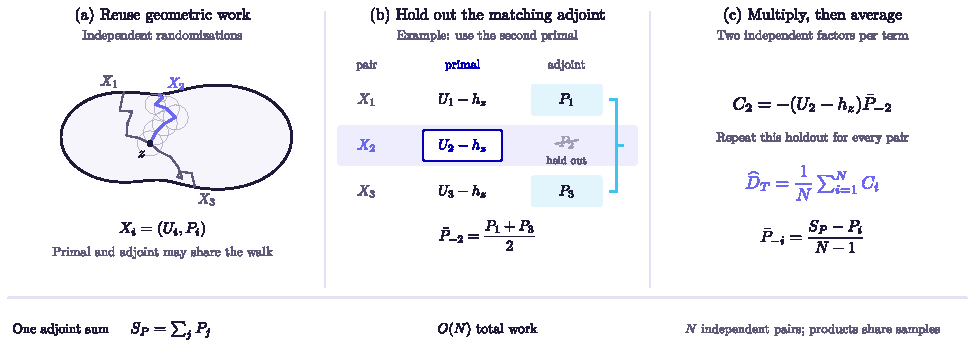
\includegraphics[width=\textwidth]{figures/crossfit.pdf}
 \caption{\textbf{A leave-one-out view of the cross-fitted estimator.} (a) Independent randomizations produce pairs $X_i=(U_i,P_i)$; both components may reuse the same walk geometry. (b) For the example $i=2$, retain $U_2-h_z$ and average the other adjoints, excluding the potentially correlated $P_2$. (c) Form $C_i=-(U_i-h_z)\bar P_{-i}$ and average over $i$. Each product has independent factors; the products themselves share samples. One adjoint sum evaluates every leave-one-out mean in $O(N)$ total work. This is exactly the estimator in \cref{eq:ustatpairwise}; unbiasedness requires unbiased marginal oracles. Walks are schematic.}
 \label{fig:crossfit}
\end{figure}

\subsection{Cross-fitted product estimator}

Define
\begin{align}
 \widehat{\DT}_N(z)
 &:=-\frac{1}{N(N-1)}
    \sum_{i\ne j}\bigl(U_i(z)-h_z\bigr)P_j(z) 
    \label{eq:ustatpairwise}\\
 &=-\frac{
   \bigl(\sum_i(U_i-h_z)\bigr)\bigl(\sum_iP_i\bigr)
   -\sum_i(U_i-h_z)P_i}
  {N(N-1)}.
  \label{eq:ustatlinear}
\end{align}
The second form costs $O(N)$ rather than $O(N^2)$.  It is a symmetric, order-two U-statistic~\cite{hoeffding1948class} with kernel
\begin{equation}
 H(X_i,X_j):=-\tfrac12\left[(U_i-h_z)P_j+(U_j-h_z)P_i\right].
 \label{eq:kernel}
\end{equation}
The factors in every cross-index product are independent, so arbitrary dependence inside $X_i$ is harmless. \Cref{thm:unbiased,thm:variance} formalize this observation. Equivalently, \cref{fig:crossfit} keeps $U_i-h_z$, pairs it with the leave-one-out mean $\bar P_{-i}=(\sum_jP_j-P_i)/(N-1)$, and averages over $i$. Only the matching $P_i$, which may share randomness with $U_i$, is omitted from that term.

\subsection{One set of paths, many candidate sites}

The algebra above is pointwise, but the optimizer must evaluate thousands of $z$ values.  The estimator permits two complementary reuse modes; our main 3D design studies use pointwise scouting, and the separate accelerated-sampling study evaluates selected reuse mechanisms:

\begin{enumerate}
  \item \textbf{Unbiased scout.}  Boundary-value caching or stochastically truncated harmonic caching turns each completed walk into a local expansion that can be queried at multiple candidates without changing its expectation~\cite{miller2023boundary,zhou2025harmonic}.  We retain the independent cache index $i$ required by \cref{eq:ustatpairwise}.
  \item \textbf{Approximate scout, bias-controlled validation.}  A low-order deterministic cache or self-normalized probe estimator may be much faster but slightly biased~\cite{huang2026probe}.  It may rank sites, but it never certifies insertion.  The selected sites are re-evaluated with fresh unbiased paths; alternatively, a proven cache bias $b_{\mathrm{cache}}$ is included in \cref{eq:certificate}.
\end{enumerate}

This separation is important.  Reusing samples after adaptively choosing the most negative noisy location produces a winner's-curse bias even when every pointwise estimator is unbiased.  For a preselected site, fresh validation avoids reusing its selection noise. Choosing again among several freshly rescored sites requires simultaneous coverage, or another independent final check, to support a certificate.

\subsection{Estimator interface}

A certifying implementation must supply the tuple
\begin{equation}
 (\widehat{\DT}_N,\ r_N(\delta),\ b_{\mathrm{term}},\ b_{\mathrm{cache}}),
 \label{eq:estimatorinterface}
\end{equation}
where $r_N$ is a statistical confidence radius and the two $b$ terms upper-bound deterministic or algorithmic bias.  The optimizer is agnostic to whether $r_N$ comes from the bounded-sample result in \cref{thm:concentration}, an empirical-Bernstein construction, or a robust median-of-means variant.  It only requires a valid coverage statement.

\section{Statistical Analysis}
\label{sec:analysis}

We now isolate the two statistical facts that make direct estimation
preferable to finite-cavity differencing: its variance contains no vanishing
geometric scale, and its uncertainty can be propagated into a valid
topological decision.  All probability statements are with respect to the
random-walk and cache randomness at a fixed candidate $z$.

\begin{theorem}[Unbiasedness under correlated pairs]
\label{thm:unbiased}
Suppose \cref{eq:oraclemeans} holds, the pairs $X_i$ are i.i.d., and the first
moments exist.  For every $N\ge2$,
\begin{equation}
 \E[\widehat{\DT}_N(z)]=\DT(z),
\end{equation}
even when $U_i$ and $P_i$ are arbitrarily dependent within a pair.
\end{theorem}

\begin{theorem}[Exact radius-independent variance]
\label{thm:variance}
Assume the oracle pairs are i.i.d. and $N\ge2$. Let $A:=U-h_z$, $B:=P$, $\mu_A:=\E A$, $\mu_B:=\E B$, and
$c_{AB}:=\Cov(A,B)$.  If $\E A^2<\infty$ and $\E B^2<\infty$, then
\begin{equation}
 \Var(\widehat{\DT}_N)
 =\frac{4}{N}\zeta_1
  +\frac{2}{N(N-1)}\zeta_2,
 \label{eq:ustatvariance}
\end{equation}
where
\begin{align}
 \zeta_1
 &=\frac14\left(
 \mu_B^2\Var A+\mu_A^2\Var B
 +2\mu_A\mu_Bc_{AB}\right),
 \label{eq:zetaone}\\
 \zeta_2
 &=\frac12\left(\Var A\,\Var B+c_{AB}^2\right).
 \label{eq:zetatwo}
\end{align}
Consequently $\Var(\widehat{\DT}_N)=O(N^{-1})$.  No term depends on an
insertion radius $\eps$.
\end{theorem}

We specialize the classical Hoeffding decomposition~\cite{hoeffding1948class};
the complete algebra appears in \cref{app:ustat}.  Correlation inside a pair can
increase or decrease the first-order variance through $c_{AB}$, but cannot
create covariance bias because the diagonal products are absent.

\begin{theorem}[Finite-sample confidence radius]
\label{thm:concentration}
Assume the unbiased i.i.d. oracle-pair hypotheses of \cref{thm:unbiased}, $N\ge2$, and $|U_i-h_z|\le M_U$ and $|P_i|\le M_P$ almost surely, and put
$M=M_UM_P>0$. Then, for every $t>0$,
\begin{equation}
 \Prob\!\left(|\widehat{\DT}_N-\DT|\ge t\right)
 \le2\exp\!\left(
 -\frac{\lfloor N/2\rfloor t^2}{2M^2}\right).
 \label{eq:hoeffdingtail}
\end{equation}
Equivalently, for every $\delta\in(0,1)$,
\begin{equation}
 \Prob\!\left[
 |\widehat{\DT}_N-\DT|
 \le M\sqrt{\frac{2\log(2/\delta)}{\lfloor N/2\rfloor}}
 \right]\ge1-\delta.
 \label{eq:hoeffdingradius}
\end{equation}
If $M=0$, the estimator and its target are identically zero, so coverage is deterministic. For $K$ candidates evaluated with arbitrary shared randomness, replacing
$\delta$ by $\delta/K$ gives simultaneous coverage.
\end{theorem}

The proof averages over all pairings of the observations and applies
Hoeffding's lemma before a Chernoff optimization; it does not treat the
$N(N-1)$ cross-products as independent.  The displayed bound is deliberately
conservative and assumption-transparent.  Experiments may additionally report
empirical-Bernstein or bootstrap intervals, but only an interval with verified
coverage may drive certification.

\subsection{Why finite-cavity differencing becomes noisy}

Consider a coupled per-path objective difference $Y_\eps=Q_\eps-Q_0$ and
independent replicates $Y_\eps^{(1)},\ldots,Y_\eps^{(N)}$.  The natural
finite-cavity estimator is
\begin{equation}
 \widehat{\DT}^{\mathrm{FD}}_{N,\eps}
 :=\frac{1}{N\rho_z(\eps)}\sum_{i=1}^{N}Y_\eps^{(i)}.
 \label{eq:fdbaseline}
\end{equation}
Common random numbers make $Y_\eps$ zero for paths whose outcome is unaffected
by the cavity.  This is useful, but it exposes a rare event.

\begin{assumption}[Rare-event coupling]
\label{ass:rareevent}
There is an event $A_\eps$ and constants $c_p,C_p,c_2,C_1>0$, independent of
sufficiently small $\eps$, such that
\begin{align}
 c_p\rho_z(\eps)&\le\Prob(A_\eps)\le C_p\rho_z(\eps),
 \label{eq:rareprob}\\
 Y_\eps&=0\quad\text{on }A_\eps^c,
 \label{eq:rarezero}\\
 \E[Y_\eps^2\mid A_\eps]&\ge c_2,
 \qquad |\E Y_\eps|\le C_1\rho_z(\eps).
 \label{eq:raremoments}
\end{align}
\end{assumption}

This captures couplings in which a path changes by $O(1)$ only when it reaches
the small cavity's influence set, whose harmonic measure is
$\Theta(\rho_z(\eps))$. The stopped-path harmonic-correction
baseline in \cref{app:submissionstudy} explicitly uses the cavity-hit event.
A generic shared-stream WoS subtraction need not vanish whenever the cavity
is missed, because its walk spheres can already differ. The rare-event
hypotheses must therefore be checked for the particular coupling; they do
not follow from shared random numbers alone.

\begin{theorem}[Rare-event variance barrier]
\label{thm:rarevariance}
Under \cref{ass:rareevent}, for every
$\eps$ satisfying
$\rho_z(\eps)\le c_pc_2/(2C_1^2)$,
\begin{equation}
 \Var[\widehat{\DT}^{\mathrm{FD}}_{N,\eps}]
 \ge \frac{c_pc_2}{2N\rho_z(\eps)}.
 \label{eq:rarevariance}
\end{equation}
Consequently, a variance bound independent of $\eps$ requires
$N=\Omega(1/\rho_z(\eps))$ paths.
\end{theorem}

This is not a universal lower bound for an importance sampler that analytically
conditions on hitting the cavity.  It is a precise diagnosis of the natural
``insert, couple, subtract, divide'' baseline.

\begin{corollary}[Candidate-map sample complexity]
\label{cor:ranking}
Under \cref{thm:concentration}, simultaneous error at most $\Delta$ for $K$
candidates with probability at least $1-\delta$ is guaranteed whenever
\begin{equation}
 \left\lfloor\frac N2\right\rfloor
 \ge\frac{2M^2}{\Delta^2}\log\frac{2K}{\delta}.
 \label{eq:directcomplexity}
\end{equation}
Thus $N=O(M^2\Delta^{-2}\log(K/\delta))$, independently of $\eps$.
Under \cref{ass:rareevent}, forcing the finite-difference variance below
$\Delta^2$ requires
\begin{equation}
 N\ge\frac{c_pc_2}{2\Delta^2\rho_z(\eps)}.
 \label{eq:fdcomplexity}
\end{equation}
\end{corollary}

\subsection{Bias bookkeeping}

The cross-fit removes correlation bias, but it cannot remove bias already
present in either marginal PDE oracle.  The next result converts marginal
bounds into a topological-derivative bias budget.

\begin{proposition}[Propagation of marginal oracle bias]
\label{prop:biaspropagation}
Suppose the pairs remain i.i.d. across indices but
\begin{equation}
 |\E U-u(z)|\le\beta_U,
 \qquad |\E P-p(z)|\le\beta_P.
 \label{eq:marginalbias}
\end{equation}
Then
\begin{equation}
 |\E\widehat{\DT}_N-\DT|
 \le |p(z)|\beta_U+|u(z)-h_z|\beta_P+\beta_U\beta_P.
 \label{eq:productbias}
\end{equation}
\end{proposition}

For unbiased Russian-roulette termination, the corresponding marginal bias is
zero.  An $\eta$-shell termination rule or a truncated cache generally has
nonzero $\beta_U,\beta_P$.  We require a conservative allocation of the right
side of \cref{eq:productbias} into
\begin{equation}
 |\E\widehat{\DT}_N-\DT|
 \le b_{\mathrm{term}}+b_{\mathrm{cache}}.
 \label{eq:biasbudget}
\end{equation}
The bounds may come from analysis or certified a posteriori residuals. A calibration-based bound must itself control reference error and allocate confidence to the calibration; a high-accuracy reference or termination-tolerance sweep alone is insufficient. A statistical interval that omits these terms does not support the general-objective guarantee in \cref{sec:optimization}. The specialized one-sided cooling validator instead uses the proved sign of its truncation bias (\cref{prop:onesidedwos}).

\section{Turning Scores into Geometry}
\label{eg:geometry}

\paragraph{Sequential design.}
We generate feasible candidates, scout with inexpensive walks, and rescore a
shortlist with fresh samples. A selected cavity is inserted, the current
domain is updated, and the process repeats. Existing interfaces can then
be refined using Differential WoS. Independent rescoring reduces selection
noise, but selecting among several fresh estimates still requires simultaneous
coverage or another final check to support a certificate. Our ranking and
refinement studies evaluate a practical heuristic; they are separate from the
guarded validation experiment below.

\begin{figure}[t]
 \centering
 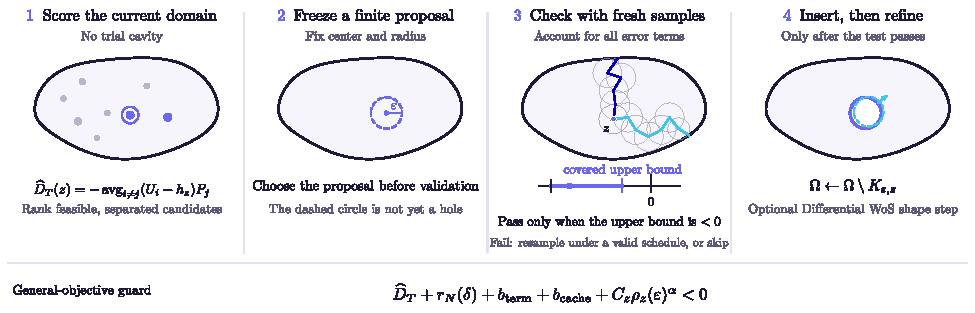
\includegraphics[width=\textwidth]{figures/pipeline.pdf}
 \caption{\textbf{From an insertion score to a finite geometric decision.} Score the current domain, freeze a center and radius, and validate with fresh samples before creating the cavity. The general-objective guard combines statistical uncertainty, oracle bias, and a finite-radius remainder bound. Its covered upper bound must be negative. A failed check leads to a valid resampling schedule or no insertion. The dashed cyan boundary shows optional subsequent shape refinement. This conditional certifying policy requires usable error bounds; the practical ranking studies and the cooling-specific finite-benefit test have separate scopes.}
 \label{fig:insertionpolicy}\label{fig:pipeline}
\end{figure}

\paragraph{General-objective acceptance.}
Suppose a known bound satisfies
\[
 |\J(\Omega_{\eps,z})-\J(\Omega)-\rho_z(\eps)\DT(z)|
 \le C_z\rho_z(\eps)^{1+\alpha}.
\]
At a preselected site, a valid statistical radius $r_N(\delta)$ and bias budget
$b=b_{\rm term}+b_{\rm cache}$ give the sufficient test
\begin{equation}
 \widehat{\DT}_N+r_N(\delta)+b+C_z\rho_z(\eps)^\alpha<0.
 \label{eg:eq:accept}
\end{equation}
The probability of accepting a non-improving insertion is then at most
$\delta$ (\cref{thm:certificate}). \Cref{fig:insertionpolicy} shows this conditional policy. A radius chosen after validation is covered
by the same event when the deterministic bound holds uniformly over allowed
radii. Existence of an asymptotic constant is insufficient: the test needs a
numerical upper bound. Across adaptive rounds, allocating summable conditional
failure probabilities controls the familywise error
(\cref{prop:freshvalidation}). Repeatedly inspecting a fixed-sample interval
without such a schedule is not covered.

\paragraph{A direct finite-benefit route for cooling.}
For $-\Delta u=f$ with bounded $0\le f\le F$ with zero Dirichlet walls in a bounded Lipschitz
three-dimensional domain $D$, let $J(D)=\int_Dfu$. A contained sphere
$\overline B_r(z)\Subset D$ has benefit
\begin{equation}
 J(D)-J(D\setminus\overline B_r(z))
 \ge 4\pi r\,(L_u-I_r^+)_+^2,
 \label{eg:eq:finitebenefit}
\end{equation}
on an event where $L_u\le u(z)$, provided
\[
I_r^+\ge\int_{B_r(z)}G_{B_r(z)}(z,y)f(y)\,dy.
\]
One may use $I_r^+=f_+r^2/6$ for a valid local upper source bound.
The difference-energy identity and the ball equilibrium potential bound the
benefit by the squared average cavity trace; the center Green identity
recovers that trace (\cref{thm:averagecertificate}). A clipped,
zero-terminal nonnegative-source WoS estimate enables a one-sided lower
confidence bound. The complete proof, sample range, and geometric guards are
in \cref{app:applicationcertificate}. The guarantee remains conditional on
the stated sampling laws and geometry assumptions.

\paragraph{Finite shape and access constraints.}
The sphere studies prescribe a count and radius, so all methods remove the
same volume. The channel study calibrates a common radius of an overlapping
ball union to a shared material budget. Strict overlap gives a positive-width
passage, while protected supports preserve the heat input. Point scoring of
a channel axis remains a finite-placement heuristic, not a derived
whole-channel topological derivative. Neither internal connectedness nor an
exterior opening implies a coolant-flow model. Detailed geometry constraints,
radius policies, and their proofs appear in the appendix.

\section{Evaluation}
\label{eg:results}

We test the estimator, the resulting finite designs, and the additional cost
of validation separately. All thermal studies use ideal zero-temperature
exterior and cavity walls. The matched design studies minimize a normalized
regional temperature with a distinct adjoint; the query study additionally
tests distributed-heating compliance, for which $p=u$. Detailed protocols, all comparisons, and step-by-step derivations are
in the appendix. The initial FEM experiment is an independent field check,
not an optimized FEM design-time baseline.

\paragraph{Actual-geometry estimator comparison.}
Eight fixed feasible sites on each of three meshes are evaluated using direct
TWoS, shared-stream finite-cavity subtraction, a stronger stopped-path harmonic
correction, and multigrid with longest-axis grid counts 49, 65, 97, and 129.
The stochastic methods use sixteen repetitions at 256 and 2,048 paths per
site. A separate sixteen-batch, 8,192-path reference estimates the infinitesimal
coefficient; it is not exact ground truth. Trial radii are 0.08, 0.04, 0.02,
and 0.01. The stronger finite-hole baseline estimates the finite correction
from a perforated-domain exit walk and a fresh original-domain state walk
only when the cavity is hit. Its exact harmonic identity and proof appear in
\cref{app:submissionstudy}.

\Cref{eg:submissionestimators} separates empirical variance from error to the
infinitesimal reference and from query time. At radius 0.01 and 2,048 paths,
the harmonic-correction variance is $35.7\times$ direct TWoS on the housing
and $13.8\times$ on the branching manifold. These are measured ratios,
not confidence bounds or fitted asymptotic laws. On the annular object,
all recorded harmonic corrections vanish at radii 0.01 and 0.02; the variance
is unresolved at this budget. We suppress the resulting collapsed bootstrap
intervals rather than interpret them as zero uncertainty. At larger radii
the stronger correction can have competitive measured variance. Multigrid
also remains a strong error--cost baseline. Finite-radius and discretization
bias are distinct from the uncertainty shown by the sampling bands.
At 2,048 paths, direct relative RMS errors are $14.9\%$, $25.2\%$, and
$146\%$; the reference's relative standard-error norms are $1.6\%$,
$4.8\%$, and $16.2\%$. The annular sparse-query case is poorly resolved
at these budgets, a limitation retained in the comparison.

\begin{figure}[tp]
 \centering
 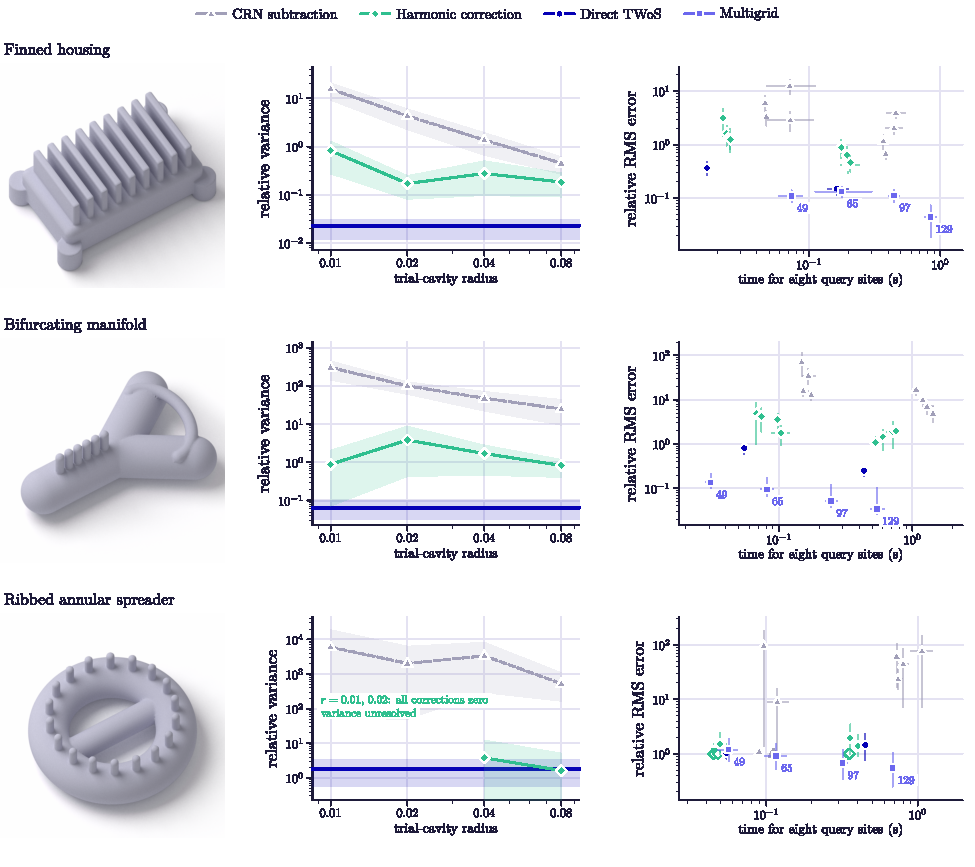
\includegraphics[width=\textwidth]{figures/submission-estimators.pdf}
 \caption{\textbf{Actual-geometry estimator comparisons.}
 Each row uses eight fixed, protected query sites on one mesh.
 The center plots normalize summed site variances by the squared norm of the
 high-budget reference and use 2,048 paths per site. Bands give pointwise 95\%
 bootstrap intervals from sixteen independent repeat vectors and sixteen
 independent reference batches. Direct TWoS has no trial-radius input;
 its horizontal band is repeated for comparison, not independently remeasured
 at every radius. Right: relative RMS error and wall time at both Monte Carlo
 budgets and all finite radii, with four deterministic grid resolutions labeled.
 Bars reflect repetition and reference-sampling uncertainty; deterministic
 grid error bars reflect only reference sampling, while their runtime bars
 use five repeated solves. Finite-radius, discretization,
 and termination biases are not enclosed. The reference is an independent,
 high-budget TWoS estimate, not exact ground truth. All-zero correction settings
 are marked unresolved and use open error--cost markers; their collapsed bootstrap intervals are suppressed.}
 \label{eg:submissionestimators}\label{fig:submissionestimators}
\end{figure}


\paragraph{Matched insertion and refinement.}
A finned housing, branching manifold, and ribbed annular spreader provide
different conduction paths. Each method inserts six disjoint radius-0.065
spheres from paired candidate pools, subject to identical source, sensor,
boundary, and pairwise clearance constraints. Every initialization then uses
the same specialized Differential WoS center-refinement component. TWoS,
multigrid at grid counts 49 and 65, and nearest-sensor placement receive eight
rounds; hottest-point and random starts receive sixteen. Five paired design
seeds are independently evaluated at saved checkpoints. This isolates the
initialization inside a shared optimizer; it does not reproduce the original
Differential WoS authors' complete application.

Mean sensor cooling after TWoS initialization and eight rounds is
$65.0\%$, $16.4\%$, and $11.4\%$ across the three objects. The primary
multigrid selector gives $65.1\%$, $16.3\%$, and $11.7\%$. Hottest-point
starts reach $42.7\%$, $0.14\%$, and $0.01\%$ despite twice as many rounds.
However, nearest-sensor placement reaches $63.6\%$, $17.3\%$, and $12.2\%$.
On the housing, complete mean times are 11.77 s for TWoS, 8.66 s for primary
multigrid, 7.99 s for coarse multigrid, and 7.08 s for nearest-sensor placement.
Thus the large benefit over hottest-point placement does not establish a
quality or speed advantage over all informed controls. The cutaways show
the stronger controls; the curves retain all six methods. Paired differences
and their pointwise intervals are reported in \cref{app:claimscope}; they do
not establish superiority over multigrid or equivalence to it.

\begin{figure}[tp]
 \centering
 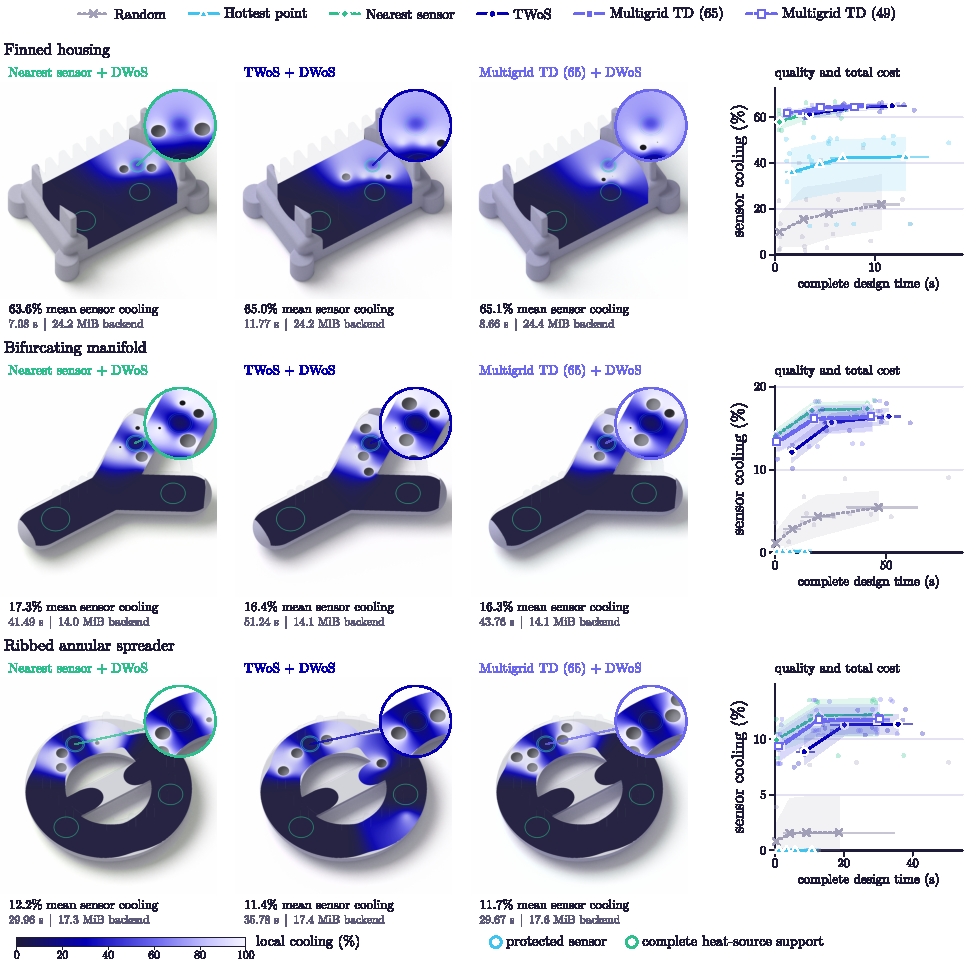
\includegraphics[width=\textwidth]{figures/submission-pipeline.pdf}
 \caption{\textbf{Insertion decisions affect the refined design.}
 Each row fixes the physical domain, protected sensor, heat input, cavity count,
 and exact removed volume. Views show the first predeclared seed after refinement;
 cyan and mint outlines mark the sensor and complete source supports. The
 section color shows local cooling relative to the unperforated temperature,
 from a common multigrid rendering field. It is not the objective's confidence
 interval. Labels and curves summarize five design seeds; faint dots show
 individual runs. Bands are pointwise 95\% bootstrap intervals for mean sensor
 cooling, jointly resampling seeds and independent evaluation blocks;
 horizontal bars resample complete runtime across seeds. Plot ranges adapt
 to each geometry; units and the local-cooling color scale are shared. They do not cover
 numerical bias. Hot and random receive up to sixteen refinement rounds;
 TWoS, both multigrid selectors, and nearest-sensor placement receive eight. Ghost shells show material
 removed only for display; some cavities lie outside the section. Independent evaluation, rendering, and mesh
 generation are excluded from design time.}
 \label{eg:submissionpipeline}\label{fig:submissionpipeline}
\end{figure}


\paragraph{Uncertainty and independent checks.}
The study contains 180 initial designs, 90 refinement runs, and 390 evaluated
states. Curves show means, individual runs, and pointwise 95\% bootstrap
intervals jointly resampling five paired design seeds and four shared
evaluation blocks. Tables additionally report the across-seed standard
deviation. These small-sample intervals exclude numerical bias. Every saved
state passes the geometric constraints, no recorded walk reaches its cap,
and the maximum multigrid relative residual is below $10^{-7}$.
Independent grid checks use 97 and 129 nodes on the longest axis; flagged
housing cases receive grids 193 and 257. The finest housing references still
differ from Monte Carlo reductions by up to 2.38 percentage points across
the checked first-seed designs, so small quality differences warrant caution.
The numerical audit does not certify reference accuracy.

\paragraph{Accessible channels at fixed material and heat input.}
Six open ball-union channels share a removed-volume target of 0.0168.
Every heat-source support is preserved, so the exact total heat input is
unchanged. Independent randomized volume audits deviate by at most 0.97\%
from the target; this is an observed audit error, not a certified bound.
TWoS gives mean regional cooling of $37.8\%$, $2.29\%$, and $1.75\%$,
versus $42.1\%$, $2.59\%$, and $1.93\%$ for primary multigrid.
Nearest-sensor placement gives $39.4\%$, $2.62\%$, and $2.02\%$.
This finite-channel heuristic is useful but does not dominate the informed
controls. Cutaways, volume audits, and full cost curves in the appendix report
the complete comparison.

\paragraph{Sparse queries at matched accuracy.}
Four meshes, two domain states, and nested batches of 8--512 fixed sites
compare TWoS against grids with 49--129 longest-axis nodes, using five paired
calibration seeds. Multigrid reuses solved fields; a stronger variant retains
outer masks and warm-starts after insertion. Compliance requires one solve.
Common mesh setup is measured separately. Our 20\% score-error target requires
an eligible upper bootstrap mean-error endpoint, MG193/MG257 refinement,
and independent Monte Carlo reference checks; it is not a continuum certificate.
A disclosed follow-up analytically integrates the prescribed sources using
classical Rao--Blackwellization (\cref{app:analytic-source}). This reduces
variance at fixed path count in ideal arithmetic, without removing termination
bias. \Cref{eg:matchedquery} compares objectives on the same Bunny; the full
protocol, ablations, reference gates, and stream correction are in
\cref{app:matchedaccuracy}.
All four calibration-selected apparent wins fail at least one confirmation
rule on 20 fresh paired seeds: three compliance cases exceed the accuracy
upper-endpoint threshold, while housing does not confirm a timing gain.
A separately declared follow-up fixes 256 walks at eight sites in both
compliance states, using 20 further fresh seeds. On the original Bunny,
TWoS takes 89.9 ms versus 113.9 ms for MG49: a $1.27\times$ ratio with
pointwise 95\% bootstrap interval $[1.05,1.50]$. Mean score error is
$9.0\%$ (upper endpoint $10.2\%$), versus $12.3\%$ for MG49.
After insertion, TWoS takes 83.1 ms versus 72.8 ms for warm-started MG;
the speed-ratio interval $[0.69,1.11]$ establishes no advantage.
This is a source-specific, eight-query result with geometry already loaded,
not a complete optimization speedup or universal state-of-the-art claim.

\begin{figure}[t]
\centering
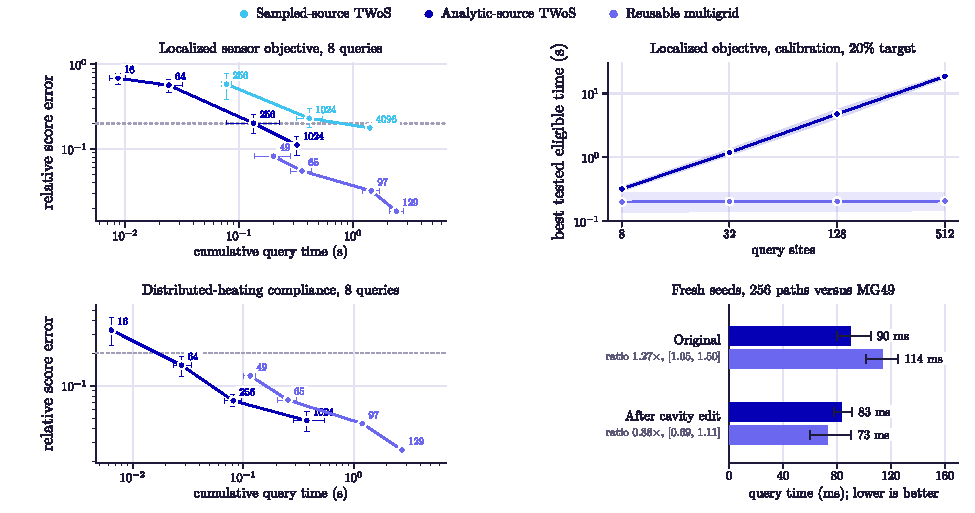
\includegraphics[width=\textwidth]{figures/matched-accuracy-bunny.pdf}
\caption{Same Bunny, different query workloads. Left: measured accuracy--cost
fronts at eight sites; labels give paths per site or longest-axis grid nodes.
Top right: fastest tested budgets passing the 20\% rule on five calibration seeds.
Bottom right: the separate fixed-budget confirmation on 20 fresh seeds; both
methods pass the 20\% error rule, but only the original-domain time ratio
confirms an advantage.
Bands and bars are pointwise 95\% bootstrap intervals; reference bias is excluded.
The analytic-source variant is restricted to the prescribed sources. Grid
curves use the faster eligible reuse implementation. Calibration fronts alone do not establish a speed claim.}
\label{eg:matchedquery}
\end{figure}

\paragraph{An exact finite-radius check.}
The uniformly heated ball with a concentric cooled cavity admits exact
states, compliance, and a positive certificate gap (\cref{app:exactcavity}).
Rational checks at 999 radii verify the algebra, not sampler coverage.

\paragraph{Validation has a separate cost.}
A guarded six-attempt compliance diagnostic on each of the Bunny and housing
uses a total failure budget of 0.01. All twelve targets pass, but validation
takes 150.39 s and 52.17 s versus 2.97 s and 0.53 s for scouting and rescoring.
Full bounds and independent checks are in the appendix. This additional
cost is excluded from ranking-only speed claims.

\section{Discussion and Limitations}
\label{sec:discussion}

The principal advantage is the direct evaluation of an insertion coefficient
using point queries on the current geometry. It is distinct from the value
of an adjoint: deterministic topological derivatives use the same objective
information, and sensor proximity is an effective alternative on our localized
tasks. The complete pipeline results do not establish a universal quality or
speed advantage. A global field can be preferable for many queries, and the
Bunny crossover should not be transferred to another geometry without measurement.

\paragraph{Choosing a solver.}
The practical question is whether the requested output is a small set of
insertion scores or a dense reusable field. Direct queries avoid trial-cavity
construction and volumetric discretization, but their work grows with the
number of queries and the required sampling accuracy. A global solve can
amortize its setup over many sites; caching and multigrid further change that
tradeoff. Our matched-target study varies the objective on the same Bunny and retains
failed fresh-seed confirmations. Localized sensor objectives can favor coarse
global solves even at eight sites. Analytic source integration helps only
within its stated source family; the sampling and reference criteria must
be satisfied before interpreting a timing advantage.
An interactive or repeatedly edited workflow remains a potential application,
not a measured speed claim of this paper.

Our objects exercise detailed boundaries, narrow gaps, branching paths, and
curved transport. They are procedural conduction benchmarks, not a representative
sample of industrial products. Zero-temperature cavities are ideal sinks,
not insulating air pockets; open channels do not solve fluid flow or conjugate
heat transfer. Fixed material and power budgets remove specific confounds
without supplying a manufacturing model. More nested cold removal lowers
compliance in this model, so costs and feature constraints are essential
to a meaningful cavity-count tradeoff.

The asymptotic theory assumes smooth domains and separated cavities; triangle
edges and ball-union seams do not literally meet its global smoothness
hypothesis. The direct compliance bound has a separate Lipschitz-domain scope.
Insulating cavities, elasticity, nonlinear PDEs, and transient problems require
their own expansions and valid oracles. Cross-fitting removes correlation bias,
not marginal solver bias. Bootstrap bands describe finite-sample uncertainty;
they do not bound discretization, termination, finite-radius, or geometry error.
The guarded validator's sampling laws still idealize pseudorandom draws and
their floating-point propagation. Its containment checks do not constitute
a verified finite-precision sampler.

\section{Conclusion}
\label{sec:conclusion}

\method{} turns classical cavity asymptotics into grid-free insertion queries.
Our analysis separates sampling variance from finite-decision error control.
Matched comparisons establish a narrow sparse-query benefit and substantial
limitations; cheaper validation and broader physical models remain open.


\FloatBarrier
\bibliographystyle{plainnat}
\bibliography{references}

\FloatBarrier
\appendix
\FloatBarrier
\section{From Scores to Finite Geometry}
\label{sec:optimization}

For a general objective, an infinitesimal derivative does not by itself guarantee that a finite cavity improves the objective. We first combine a uniform finite-size remainder with statistical and algorithmic uncertainty, then give a direct quantitative certificate for the cooling model.

\begin{assumption}[Usable finite-radius remainder]
\label{ass:remainder}
For every admissible candidate $z$ and $0<\eps\le\eps_0$, a known or
conservatively bounded $C_z>0$ and $\alpha>0$ satisfy
\begin{equation}
 \left|\J(\Omega_{\eps,z})-\J(\Omega)
 -\rho_z(\eps)\DT(z)\right|
 \le C_z\rho_z(\eps)^{1+\alpha}.
 \label{eq:remainderbound}
\end{equation}
\end{assumption}

For the model analyzed in \cref{sec:problem},
\cref{thm:localtd} establishes the existence of such a remainder bound with $\alpha=1$ in two dimensions
and $\alpha=1/2$ in three dimensions.  Certification additionally requires a
numerical upper bound on $C_z$, rather than only its existence.

\begin{theorem}[Certified finite insertion]
\label{thm:certificate}
Suppose \cref{ass:remainder,eq:biasbudget} hold and, with probability at least
$1-\delta$,
\begin{equation}
 |\widehat{\DT}_N-\E\widehat{\DT}_N|
 \le r_N(\delta).
 \label{eq:validationcoverage}
\end{equation}
If
\begin{equation}
 \boxed{
 \widehat{\DT}_N(z)+r_N(\delta)
 +b_{\mathrm{term}}+b_{\mathrm{cache}}
 +C_z\rho_z(\eps)^\alpha<0,}
 \label{eq:certificate}
\end{equation}
the probability of accepting a non-improving insertion is at most $\delta$. Equivalently, on an event of probability at least $1-\delta$, the test implies $\J(\Omega_{\eps,z})<\J(\Omega)$. This is an error-control statement, not a posterior probability conditional on acceptance.
\end{theorem}

\begin{corollary}[Data-dependent radius selection]
\label{cor:adaptiveradius}
Assume \cref{eq:remainderbound} holds simultaneously for all
$\eps\in(0,\eps_0]$.  On the basis of the validation batch, let
$\widehat\eps\in(0,\eps_0]$ be any measurable radius satisfying
\cref{eq:certificate}.  Then, on an event of probability at least $1-\delta$, acceptance implies
$\J(\Omega_{\widehat\eps,z})<\J(\Omega)$. Equivalently, the probability of accepting a non-improving radius is at most $\delta$. No union bound over radii is needed.
\end{corollary}

The certificate separates sampling error, termination bias, cache bias, and
the asymptotic remainder.  If it fails, one can sample more, improve the PDE
oracle, reduce $\eps$, or reject the site.

\subsection{Certifying a useful amount of improvement}
\label{sec:minbenefit}

For ideal zero-Dirichlet cooling, adding a feasible cavity already lowers
compliance by monotonicity (\cref{prop:coolingmonotonicity}). The useful
certification target is therefore a \emph{minimum finite benefit}, optionally
large enough to pay an explicit insertion cost.

\begin{theorem}[Minimum benefit from a topological score]
\label{thm:minbenefit}
Under the hypotheses of \cref{thm:certificate}, set
$b=b_{\rm term}+b_{\rm cache}$. With probability at least $1-\delta$, the
actual benefit $B=\J(\Omega)-\J(\Omega_{\eps,z})$ satisfies
\begin{equation}
 \begin{split}
 B&\ge\underline B_{\rm TD}(z,\eps),\\
 \underline B_{\rm TD}
 &=-\rho_z(\eps)\bigl[\widehat{\DT}_N+r_N(\delta)+b\bigr]
   -C_z\rho_z(\eps)^{1+\alpha}.
 \end{split}
 \label{eq:minimumbenefit}
\end{equation}
The event is simultaneous over radii covered by the uniform remainder.
Accepting only when $\underline B_{\rm TD}\ge\tau$ controls the probability
of accepting an insertion with benefit below $\tau$ by $\delta$.
\end{theorem}

This route still requires numerical bounds on capacity, bias, and remainder;
\cref{app:minbenefit} handles certified capacity intervals explicitly. For
three-dimensional Poisson compliance, a variational argument supplies a
second route with explicit finite-radius constants.

\Needspace{17\baselineskip}
\begin{theorem}[Direct finite-hole cooling benefit]
\label{thm:coolingbenefit}
Let $D\subset\R^3$ be bounded and Lipschitz, let $0\le f\le F$ be bounded,
and let $-\Delta u=f$ on $D$ with zero Dirichlet data. Define
$J(D)=\int_Dfu$. Suppose $\overline B_R(z)\Subset D$ and known local bounds
$0\le f_-\le f\le f_+$ hold on $B_R(z)$. If
$\Prob\{L_u\le u(z)\}\ge1-\delta$, then simultaneously for all $0<r<R$,
with probability at least $1-\delta$,
\begin{equation}
 \begin{split}
 J(D)-J(D\setminus\overline B_r(z))
 &\ge\underline B_{\rm cool}(z,r):=4\pi r\,m^2,\\
 m&=\frac{f_-(R^2-r^2)}6\\
 &\quad+\frac{1-r/R}{(1+r/R)^2}
       \left(L_u-\frac{f_+R^2}6\right)_+.
 \end{split}
 \label{eq:directcoolingbenefit}
\end{equation}
Here the new cavity also has zero Dirichlet data. Accepting only if this
lower bound exceeds a chosen target gives the same false-acceptance control
as \cref{thm:minbenefit}.
\end{theorem}

The proof combines the exact compliance difference-energy identity with
ball capacity and a Poisson-kernel comparison; it needs no unknown
asymptotic remainder. A finite, zero-terminal WoS walk with nonnegative
source samples has expectation at most $u(z)$, enabling a one-sided
confidence bound with a fully explicit sample range
(\cref{prop:onesidedwos}). Setting $L_u=0$ instead yields a deterministic
source-only bound. These conservative bounds can fail to reach the requested
target even when an insertion is beneficial. \Cref{app:minbenefit} proves
all steps, explicit cost and relative-benefit rules, and adaptive selection
control. The manufactured check in \cref{app:benefitcheck} tests the formulas;
the earlier Bunny and housing runs evaluate the ranking implementation. A separate application validation study is reported in \cref{sec:applicationvalidation}.

\begin{theorem}[Average-trace finite-hole certificate]
\label{thm:averagecertificate}
Under the cooling hypotheses of \cref{thm:coolingbenefit}, suppose a known $I_r^+$ satisfies
\[
 I_r^+\ge\int_{B_r(z)}G_{B_r(z)}(z,y)f(y)\,dy.
\]
On the same
state-coverage event, simultaneously for contained radii,
\begin{equation}
 B(z,r)\ge\underline B_{\rm avg}(z,r)
 :=4\pi r\,(L_u-I_r^+)_+^2.
 \label{eq:averagecertificate}
\end{equation}
One may use $I_r^+=f_+r^2/6$ with an upper source bound on $B_r(z)$.
For affine $f$, the exact source integral is $f(z)r^2/6$.
\end{theorem}

The proof pairs the state-difference energy with the ball's equilibrium
potential, bounding benefit by the squared \emph{average} cavity trace;
the center Green identity recovers that average. The application validator
uses the maximum of this bound and the preceding temperature-floor bound.
\Cref{app:applicationcertificate} derives this identity, the clipped-walk
validator, geometric guards, and the separate application experiment.

\subsection{Scout--rank--validate--refine}

One outer iteration is:
\begin{enumerate}
 \item \textbf{Scout.} Generate candidates in free space subject to boundary
 clearance.  Evaluate a cheap \method{} map using shared unbiased caches or a
 deliberately approximate ranking cache.
 \item \textbf{Rank.} Keep the $m$ most promising spatially separated
 candidates.  Non-maximum suppression avoids repeatedly validating one basin.
 \item \textbf{Validate.} Fix one finalist using only the scouting and ranking data, then draw a separate validation batch. Alternatively, validate several survivors and allocate confidence across that entire shortlist. Use a valid bias bound for the general-objective route or the one-sided construction for cooling. A sequential implementation must use either
 an anytime-valid confidence sequence or a predeclared stage schedule
 $N_1<N_2<\cdots$ with error levels whose sum is at most the candidate's
 allocated failure probability; a fixed-$N$ interval may not be repeatedly
 inspected under optional stopping.
 \item \textbf{Insert.} Choose the site with the largest covered benefit bound meeting the
 target (and any explicit cost), and instantiate $K_{\eps,z}$.  If no site is certified, perform
 only shape refinement or terminate.
 \item \textbf{Refine.} Move existing interfaces using Differential WoS or
 derivative WoSt~\cite{miller2024differential,yu2025robust}, with a line search
 on independently estimated objective values.
\end{enumerate}


\begin{proposition}[Adaptive selection across candidates and rounds]
\label{prop:freshvalidation}
Let $(\mathcal F_t)_{t\ge0}$ be the history of the optimizer.  At validation
round $t$, let the scout choose $(Z_t,\eps_t)$ using only
$\mathcal F_{t-1}$, and let a fresh validation procedure produce an event
$E_t$ such that
\begin{equation}
 \Prob(E_t^c\mid\mathcal F_{t-1})\le\delta_t
 \quad\text{almost surely}.
 \label{eq:conditionalcoverage}
\end{equation}
If the implementation accepts only when the observable test
\cref{eq:certificate} holds, and $E_t$ is its valid coverage event, then
\begin{equation}
 \Prob(\text{some accepted insertion is non-improving})
 \le\sum_{t\ge1}\delta_t.
 \label{eq:sequentialfamilywise}
\end{equation}
Here $t$ indexes individual preselected candidate tests. If a round selects
among several validation estimates, coverage must hold simultaneously for that
shortlist, for example by allocating $\delta_t/m$ to each of $m$ candidates.
Shared randomness across candidates is allowed; fresh data alone does not
remove selection error within the validation shortlist.
\end{proposition}

\subsection{Practical placement and connected refinement}

The original box, Bunny, and housing ranking experiments prescribe the number and radius of cavities and use fresh shortlist estimates to rank finite insertions. Their heuristic uses lower confidence scores but supplies neither a numerical remainder bound nor full coverage after selection. These experiments therefore evaluate placement quality, not the finite-insertion certificate. The count--volume study varies prescribed radii across allocations; it optimizes centers, not individual radii.

For connected geometry, we select two interior terminals using topological scores and join them by a weighted candidate graph. The path initializes an overlapping ball union. Strict consecutive-ball overlap is enforced after each radius recalibration, so the removed interior is path connected. Differential WoS then proposes motions of its controls, and fresh paired objective estimates assess trial steps. This graph initialization is a finite geometric heuristic: the single-cavity theorem does not certify simultaneous insertion of the whole channel. Its endpoints remain internal, so connectedness does not imply exterior cooling access. \Cref{app:channelimplementation} gives the parameterization, regularity assumptions, chain rule, discrete volume calibration, and conditional shape-acceptance result.

\subsection{Choosing a finite radius}

After estimating $\DT$, choose an admissible $\eps$ satisfying the minimum-benefit test, clearance constraints, and a manufacturing lower bound. For example, maximize the covered net-benefit bound over the allowed radii; the largest feasible radius need not maximize that bound.
\Cref{cor:adaptiveradius} shows why this data-dependent choice is valid: the
same confidence event controls every radius because the deterministic remainder
bound is uniform in $\eps$.  A higher-order asymptotic estimate may permit a
larger step, but the leading-order certificate remains the fallback.

\subsection{Multiple insertions}

The single-hole expansion does not justify inserting many nearby cavities at
once.  The proved policy is sequential: validate and insert one cavity, update
the domain, then condition on that history and validate the next one using a
fresh batch.  This is covered by \cref{prop:freshvalidation}.  Simultaneous
insertion requires a separate uniform interaction bound and is not claimed by
the present theorem.

\FloatBarrier
\section{Evaluation}
\label{sec:results}

We evaluate three claims: direct estimation avoids shrinking-target noise; local scores support useful cavity placement; and sparse queries can reduce computational cost relative to a global discretized solve. Matched pipelines on a finned housing, branching manifold, and annular spreader test placement and numerical cost under shared constraints. The Bunny supplies a detailed-geometry stress test and a count--radius study, while controlled experiments isolate statistical effects. Earlier thermal studies retain their original protocols and are summarized separately. \Cref{app:experiments,sec:critical} retain full protocols, secondary plots, solver checks, and all measured comparisons.

\paragraph{Common physics and decision rule.}
All 3D design studies solve $-\Delta u=f$ with nonnegative internal heating and ideal zero-temperature exterior and cavity walls. The sensor-protection pipelines and accessible-channel studies minimize the regional objective $J_q=\int qu/\int q$ with a distinct adjoint; the compact sensor weight in the new matched study is normalized to integrate to one. The earlier Bunny, housing-compliance, and guarded-validation studies minimize compliance $J=\int fu$ under prescribed removal and clearance constraints. Their relative reductions use a fixed original-domain normalization and fresh objective samples. For compliance, $p=u$ and the candidate benefit is $u^2$; a cross-fitted score uses distinct walk indices even when the same samples represent both fields. Each insertion changes the domain before the next score evaluation. The ranking studies use fresh shortlist samples. \Cref{sec:applicationvalidation} separately evaluates a guarded compliance selector.

\paragraph{Measured comparisons.}
The deterministic design baselines use a voxel adjoint field with either conjugate gradients or geometric multigrid; they evaluate the same topological score and share the candidate and cavity budgets. Random feasible placement tests whether the score helps beyond adding cold surface. Same-seed multiplication and finite-cavity differencing isolate estimator choices. Array-RQMC and neighbor reuse are studied separately as compatible accelerations. The external FEM experiment checks initial fields, and the probabilistic-shape and spectral-connectivity experiments check components; none is presented as a reproduced full external optimizer.

\subsection{Matched design pipelines on distinct geometry}
\label{sec:submissionstudy}

We next isolate three questions that a cavity-count comparison alone cannot
answer: whether objective-aware nucleation improves subsequent boundary
optimization; whether accessible-channel improvements survive fixed material
and power budgets; and whether the shrinking-target comparison transfers to
actual three-dimensional application meshes. The finned housing, branching
manifold, and ribbed annular spreader in \cref{fig:submissiongeometries} have
narrow gaps, branching paths, or curved transport and a thin central bridge.
Their protected sensors and complete compact heat-source supports remain
unchanged under every design. \Cref{app:submissionstudy} specifies the physics,
normalizations, geometry constraints, and numerical checks.



\paragraph{Nucleation followed by Differential WoS.}
All methods place six disjoint spheres of radius $0.065$ from the same paired
candidate pools, then optimize their centers using a common specialized
implementation of Differential WoS~\cite{miller2024differential}.
TWoS and deterministic topological derivatives use eight refinement rounds;
hottest-point and random initializations also receive rounds nine through
sixteen. Two complete deterministic baselines use longest-axis grid counts
49 and 65. A nearest-sensor control replaces the PDE score by Euclidean
distance to the protected sensor and receives eight refinement rounds. The curves in \cref{fig:submissionpipeline} report complete design
costs at independently evaluated checkpoints. This comparison isolates the
value of initialization inside a shared optimizer; it does not compare against
the original authors' full application or assert that Differential WoS cannot
change topology.

Across five paired seeds, TWoS followed by eight refinement rounds yields
mean sensor reductions of $65.0\%$, $16.4\%$, and $11.4\%$ on the housing,
branching manifold, and annular spreader. The primary multigrid selector followed
by the same refinement yields $65.1\%$, $16.3\%$, and $11.7\%$.
Hottest-point initialization with sixteen rounds yields $42.7\%$, $0.14\%$,
and $0.01\%$, respectively. Both TD selectors perform similarly in these
comparisons; their numerical costs and the additional controls are reported
in the full time--quality curves and \cref{tab:submissionpipeline}.
The nearest-sensor control yields $63.6\%$, $17.3\%$, and $12.2\%$
across the same three objects. On the housing it requires $7.08$ s, compared
with $11.77$ s for TWoS.
Thus the large contrast with hottest-point placement does not establish a
large benefit over every informed heuristic. The cutaways show this stronger
geometric control alongside TWoS and multigrid; the plots retain all methods.
The bands describe uncertainty in measured mean cooling, not equivalence tests
or guarantees for a new geometry.


\paragraph{Accessible channels at matched volume and fixed power.}
Six parallel open ball-union channels target total removed volume $0.0168$.
Their common radius is recalibrated after each insertion, and independent
scrambled-Sobol samples audit the final volume. All heat supports are protected,
so their exact input power is invariant (\cref{prop:protectedpower}).
\Cref{fig:submissionchannels} reports these finite designs. A pointwise
axis score initializes the channels; it is not a topological derivative of
an entire channel, and the radius calibration is numerical rather than certified.
At this matched budget, TWoS yields mean reductions of $37.8\%$, $2.29\%$,
and $1.75\%$ across the three objects, compared with $42.1\%$, $2.59\%$,
and $1.93\%$ for the primary multigrid selector. On the housing, nearest-sensor
placement yields $39.4\%$, and the cheaper multigrid grid attains the same
mean reduction as the primary grid. Thus this finite-channel heuristic does
not dominate the informed controls. \Cref{tab:submissionchannels} reports all
methods and uncertainty intervals; the independent volume and reference audits
remain separate from those sampling intervals.

\paragraph{Variance, bias, and query cost.}
\Cref{fig:submissionestimators} compares direct scores, common-random-number
finite-cavity subtraction, a stronger stopped-path harmonic-correction
baseline, and multigrid at four resolutions on eight fixed sites per object.
Sixteen independent repeats resolve sampling variability. Relative variance
about each method's mean is shown separately from error to a high-budget
infinitesimal reference: finite-cavity methods retain finite-radius bias,
while multigrid retains discretization error. The reference itself has
sampling and termination error. Bands around variance describe uncertainty
in the estimated variance, not a standard-deviation envelope of field values.
\Cref{app:submissionstudy} gives the stronger finite-correction identity and
its step-by-step proof; detailed numeric summaries accompany the source.
At radius $0.01$ and 2,048 paths per site, the stronger harmonic-correction
baseline has $35.7\times$ and $13.8\times$ the measured direct variance on
the housing and branching object. These are point estimates, not confidence
bounds. On the annular object, all recorded harmonic corrections vanish at
radii $0.01$ and $0.02$; variance is unresolved, and collapsed bootstrap
intervals are suppressed. At larger radii the stronger correction can have
competitive measured variance. Direct TWoS relative RMS error at this budget
is $14.9\%$, $25.2\%$, and $146\%$ across the three cases, while the
reference's relative standard-error norms are $1.6\%$, $4.8\%$, and
$16.2\%$. The annular sparse-query configuration is poorly resolved at these
budgets; it is not evidence of uniformly accurate pointwise estimation.

The maximum independent channel-volume audit deviation is $0.97\%$ of the
target. Finer housing checks change by at most $0.44$ percentage points from
grid 193 to 257, but MC--grid257 differences still reach $2.38$ points across
the checked first-seed states. Sampling intervals do not absorb this numerical
reference sensitivity (\cref{tab:submissionfinereference}).


\subsection{Protecting a region with a distinct adjoint}
\label{sec:regional}

Compliance makes the adjoint equal to the state. To test whether
objective-aware scoring matters beyond finding hot spots, we keep the
housing's heat sources fixed and minimize the weighted mean temperature
of a protected sensor region. The objective is
$J_q=\int q u/\int q$, where $q$ is a compact nonnegative bump in
a radius-$0.13$ ball. The adjoint solves $-\Delta p=q$, and candidates
are ranked by $up$. This differs from the hottest-point score $u$.
Two sensor placements test the left and right sides of the same housing;
they are two objectives, not two independent input geometries.
All cavities must avoid the sensor region with an additional $0.02$
gap, so no design can improve the objective by deleting the sensor.
\Cref{app:regional} derives the normalization, adjoint, and an exact
counterexample to hottest-point placement.

Each of five paired candidate/design seeds supplies 768 candidates.
Every method places six radius-$0.095$ cavities under the same clearance
constraints. We compare sparse \method{} (12 scouting and 192 rescoring
walks), a larger budget (48 and 768), WoS hottest-point placement at the
sparse budget, deterministic multigrid hottest-point placement,
multigrid topological derivatives, and random feasible placement.
The 24-site rescore uses fresh walks. Paired state--adjoint queries
share paths within each pair and use the cross-index product.
Multigrid reuses one geometry hierarchy for its two right-hand sides.
The primary grid is $113\times73\times57$; a supplementary sweep
adds $57\times37\times29$, $85\times55\times43$, and
$169\times109\times85$ without discarding unfavorable results.

Sparse \method{} reduces the left/right regional objectives by $50.87\%$ /\allowbreak $50.09\%$, compared with $38.15\%$ /\allowbreak $29.99\%$ for deterministic hottest-point placement. The primary multigrid topological selector gives $53.30\%$ /\allowbreak $52.15\%$. Averaged across both cases, complete sparse \method{} design takes $3.66$\,s, versus $8.38$\,s for the primary multigrid setting. The fastest tested multigrid setting (57 nodes along the first axis) takes $2.51$\,s and gives $53.50\%$ /\allowbreak $52.53\%$ reduction. Retaining the outer mesh in one process per complete adaptive design reduces wall time to $1.22$\,s for sparse \method{}, $1.41$\,s for coarse multigrid, and $7.13$\,s for primary multigrid. All 70 repeated designs have exactly the same six sequential cavity centers as their original runs, permitting reuse of the independent objective evaluations. These results demonstrate an advantage over hottest-point placement; the full budget sweep in \cref{fig:regional,tab:regional} qualifies comparisons with volumetric topological derivatives.


Complete design wall times include common candidate preparation,
geometry setup, source queries or PDE solves, candidate filtering,
ranking, subprocess startup, and file I/O. The retained-mesh backend
keeps the fixed outer boundary acceleration structure alive throughout
each six-round design, for both Monte Carlo and multigrid methods.
Candidate filtering, fresh rescoring, and every adaptive insertion still
execute inside the measured driver; future requests are not replayed
ahead of those decisions. Offline reference evaluation
is measured separately. Both a fresh WoS evaluation and a separate
$169\times109\times85$ multigrid solution assess every final design.
These are approximate references; first-seed designs additionally
receive a fourfold WoS shell refinement and a $225\times145\times113$
grid check. The designs use fixed-count ranking, not the
compliance-only finite-benefit certificate. The comparison against
hottest-point placement tests the adjoint's value, which is shared
with deterministic topological derivatives; the quality--cost
comparison tests the choice of numerical estimator.



\subsection{Accessible channels and protected components}
\label{sec:accessible}
We next replace sealed cavities with vertical through-channels in the
housing. Every channel is a union of 18 radius-$0.075$ balls, spanning
both exterior sides. Their spacing gives a guaranteed continuous
passage of radius $0.075\sqrt{3}/2$; \cref{app:accessible} proves this
geometric statement and the component-clearance predicates. The
sensor and three prescribed component regions cannot be removed.
Port positions vary with the selected axes. We retain the ideal cold-wall
model, so geometric access does not establish coolant delivery or
realistic heat transfer.

This is an application of point scoring to a larger geometric operation:
the algorithm scores candidate axes at a common interior plane and
inserts the complete channel. The pointwise topological coefficient
is a placement proxy here, not a derived whole-channel derivative.
All five methods use the same candidate axes, six-channel count,
radius, extent, and protection constraints. We repeat both sensor
objectives over five paired seeds and evaluate all 50 completed
designs independently. Removed volume is reported because local
housing thickness varies; this is not an equal-volume experiment.

On the left and right sensors, the TWoS proxy gives reductions of $55.74\%$ and $52.47\%$, versus $43.78\%$ and $30.39\%$ for hottest-point placement. Mean complete design times are $1.02$\,s for TWoS and $1.26$\,s for coarse multigrid. Their mean reductions across both sensors are $54.10\%$ and $57.55\%$, respectively. This preserves a useful quality--cost tradeoff under access constraints, without establishing superiority over deterministic topological scoring.





\subsection{Thermal design on a finned housing}

A closed 96,740-triangle procedural housing contains three localized Gaussian heat sources. Each method places six radius-$0.095$ cavities from 768 shared Sobol candidates. Sparse \method{} uses 12 scouting walks per feasible site and 192 fresh walks on a 24-site shortlist; a larger budget uses 96 and 768 walks. A predeclared field-error criterion selects the multigrid grid, $113\times73\times57$, from a resolution sweep. Both algorithms run in the same C++ executable. Selection time includes geometry acceleration and all six rounds of querying or global solving; it excludes file I/O, process startup, and the common independent objective evaluation.



Across five complete stochastic design seeds, sparse \method{} reduces compliance by $68.90\%\pm0.84\%$ (standard error), compared with $70.36\%\pm0.08\%$ for the deterministic multigrid design, whose uncertainty comes from objective evaluation. Mean selection time is $0.432$ s versus $1.861$ s: $4.31\times$ faster while achieving $97.9\%$ of the measured reduction. The larger \method{} budget gives $69.39\%\pm0.51\%$ reduction in $1.731$ s, using $19.1$ MiB peak RSS versus $31.4$ MiB. Random placement gives $27.76\%\pm4.57\%$. These are quality--cost tradeoffs over the tested designs; the seed count does not establish equivalence or superiority in design quality. The multigrid sweep and resource curves appear in \cref{fig:housingtradeoffs}. This earlier compliance comparison uses a field-error-selected grid and excludes driver costs; the regional pipelines in \cref{sec:submissionstudy} include those costs and both cheaper grids. Its speed ratio should not be transferred between these protocols.

An independent scikit-fem implementation on 393,616 tetrahedra checks the initial ranking. The 512-walk field has Pearson correlation $0.9943$ and $95\%$ top-20 overlap with that FEM field. Its boundary approximation and convergence are documented in \cref{fig:externalaudit}; the FEM audit is an accuracy comparison, not an optimized FEM timing baseline.

\subsection{Detailed geometry and sparse-query scaling}

We repair and close the Stanford Bunny~\cite{stanford1994bunny}, obtaining 69,674 triangles, and normalize its height to one. With affine heating $f(x,y,z)=1+0.65(y+0.5)$, each method places six radius-$0.05$ cavities among 1,024 candidates. \method{} uses a 12-walk scout and fresh 128-walk rescoring of 20 sites. Its measured compliance reduction is $47.77\%$, compared with $48.06\%$ for the $54\times64\times48$ voxel adjoint and $39.46\%$ for random placement. This single-run test demonstrates placement on detailed geometry; the replicated allocation study below supplies a broader design comparison.

A separate matched C++ experiment isolates query cost on the original Bunny. At 64 requested sites, 512-walk \method{} takes $0.381$ s and $15.4$ MiB peak RSS; voxel FD/CG takes $0.528$ s and $80.7$ MiB. The corresponding relative score errors against an independent 16,384-walk reference are $5.89\%$ and $6.89\%$. This is $1.39\times$ faster evaluation with $81\%$ less peak memory, at similar measured error. The numerical reference itself has sampling and termination error. The methods tie near 96 sites, and at 384 sites the voxel solve is faster ($0.504$ s versus $2.10$ s). \Cref{fig:compiledbunny} reports the full sweep. These timings establish a sparse-query advantage, not a speedup for the displayed Bunny optimization.



\subsection{Cavity count at fixed removed volume}
\label{sec:bunnybudget}

Does cooling improve because placement is better, or simply because more
material is removed? We separate these effects with 72 Bunny designs:
two exact volume budgets, four counts $n\in\{2,4,6,12\}$, three independent
design seeds, and \method{}, voxel-adjoint TD, and random feasible placement.
The budgets equal three or six radius-$0.05$ balls: $0.765\%$ or $1.529\%$
of the original Bunny volume. Within each allocation, every cavity has
radius $r_n=0.05(b/n)^{1/3}$, where $b\in\{3,6\}$ is the budget in ball-volume
units. Radii follow this constraint; only centers are optimized. All methods
share 1,024 candidates within each seed/allocation, retain outer clearance
$0.012$ and pairwise surface gap $0.014$, and start from the unperforated domain.
TWoS retains the 12-walk scout and independent 128-walk shortlist rescoring;
this ranking heuristic is not a finite-insertion confidence certificate.
The compiled voxel selector uses a finer $96\times112\times84$ FD/CG grid
than the original Bunny design test.



% The following measured paragraph is populated from the retained summaries.
At the full volume budget, increasing the TWoS count from two to twelve raises mean cooling from $37.58\%$ to $54.33\%$, while the radius decreases from $0.0721$ to $0.0397$. At twelve cavities, the voxel and random means are $55.02\%$ and $38.78\%$, respectively. The most useful allocation comparison is across budgets: twelve small TWoS cavities at half volume yield $47.26\%$ cooling (design range $47.03$--$47.67\%$), versus $47.45\%$ ($46.78$--$48.22\%$) for six larger cavities at full volume. The former also has $20.6\%$ less cavity surface area, by exact sphere geometry. This is similar measured cooling with less removal, not a proved equivalence or an advantage unique to TWoS. The voxel selector shows a similar allocation trend. A fourfold thinner WoS termination shell, $1.25\times10^{-4}$, changes cooling by at most $0.204$ percentage points for the pre-specified first-seed full-budget endpoint designs from both TD selectors. This sensitivity check does not bound the remaining bias.
An additional first-seed check of the half-volume comparison, chosen after inspecting the allocation results, gives $46.88\%$ versus $47.21\%$ cooling with the thinner shell, respectively.


All objective comparisons use four independently scrambled 512-point
interior blocks and 128 WoS paths per active point, separate from selection.
Removed material contributes zero under fixed original-volume normalization;
reported percentages average paired block ratios to the initial state.
Design ranges and conditional block standard errors are retained separately;
three seeds do not establish equivalence or a globally optimal allocation.

\paragraph{Why a preferred count needs a cost.}
Additional nested ideal cooled removal lowers compliance exactly
(\cref{prop:coolingmonotonicity}), whereas different equal-volume allocations
are not nested. At fixed removed volume $V$, exposed area grows as $n^{1/3}$
and the sum of isolated capacities as $n^{2/3}$ (\cref{prop:budgetgeometry});
the latter is not the interacting union capacity. A volume-only penalty is
constant within this sweep. Instead, \cref{fig:bunnybudget}c illustrates
$J/J_0+\kappa n$ for an explicitly assumed count cost. This isolates the
modeling choice behind a ``sweet spot'' without attributing it to the
topological estimator or claiming an application-specific optimum.


\subsection{Estimator accuracy and sampling uncertainty}

The annulus diagnostic has an exact capacity and cavity-hit probability, making the rare-event comparison analytically controlled. With 256 samples per estimate and 3,000 repetitions, fitted variance slopes versus capacity are $0.00$ for direct estimation, $-1.10$ for coupled differencing, and $-1.89$ for independent differencing. At the smallest tested capacity, direct variance is $8.26\times$ lower than the coupled baseline. This experiment tests the shrinking-target mechanism under its stated model; it does not rule out importance samplers conditioned on cavity hits.

\begin{figure}[t]
 \centering
 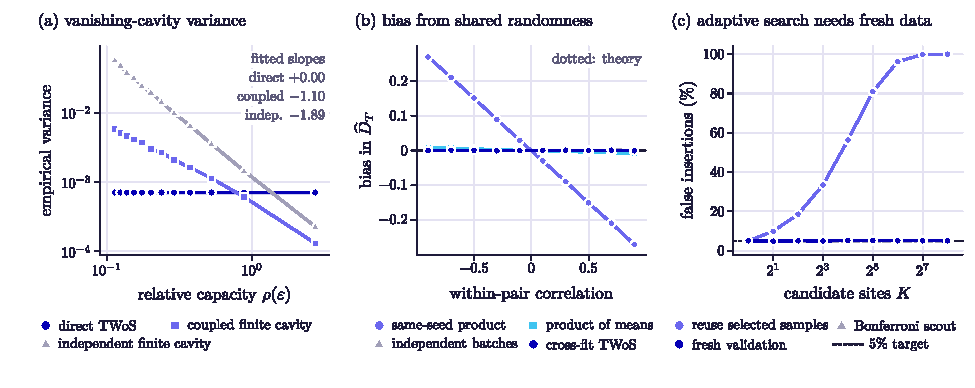
\includegraphics[width=\textwidth]{figures/controlled-experiments.pdf}
 \caption{Controlled tests of the statistical claims. (a) Direct \method{} has no insertion-radius input, so its measured variance is constant; coupled finite-cavity differencing follows the predicted $\rho^{-1}$ rare-event law, while independent solves approach the worse $\rho^{-2}$ law. Shading gives 95\% bootstrap intervals. (b) Same-seed multiplication inherits the full covariance bias and the product of sample means retains $1/N$ of it. The leave-diagonal-out estimator remains unbiased up to Monte Carlo error; independent batches are the unbiased no-reuse reference. (c) Reusing the most negative scout loses nominal coverage as the candidate count grows. Fresh validation and a simultaneous Bonferroni scout both meet the 5\% target; fresh validation controls the preselected-site test in this known-noise diagnostic.}
 \label{fig:controlled}
\end{figure}

Correlated-pair tests confirm the covariance bias predicted for same-index products. Cross-fitting and fully independent primal/adjoint batches both remove it; cross-fitting is not uniformly lower variance. The manufactured harmonic fields in \cref{fig:manufactured} test this product algebra spatially. A separate Poisson-compliance disk test has a genuine analytic topological derivative, $D_T(z)=-(1-|z|^2)^2/16$. There, independently randomized Array-RQMC batches reduce MSE by $19.9\times$ relative to ordinary Monte Carlo at equal path count, while taking longer in the measured Python implementation (\cref{fig:accelerated}). Statistical efficiency and runtime are reported separately.

The adaptive-selection test uses null candidates with known Gaussian noise. Selecting and testing with the same samples produces almost certain false acceptance among 256 sites; fresh validation and simultaneous Bonferroni bounds produce rates near the nominal $5\%$. This isolates selection error. It does not measure coverage for finite 3D insertions. The general-objective certificate also requires numerical remainder and bias bounds; the specialized cooling validator is evaluated separately below.

\subsection{Compatibility with connected refinement}

On the housing, a topological-score-weighted candidate graph initializes a connected 22-ball cavity between two internal terminals. Every trial enforces strict overlap and the same fixed-Sobol removed volume. Six Differential WoS refinement rounds propose control-point motions; fresh paired Student-$t$ tests with a Bonferroni allocation accept three steps. Independent evaluation reports a $2.086\%$ objective decrease from the graph initialization. The graph initialization itself does not measurably outperform the straight connection in this example. The channel remains sealed inside the housing, and the interval coverage relies on the paired-normal model. This experiment demonstrates compatibility between cavity initialization and existing-boundary refinement; it does not establish accessible coolant routing or a certified global topology optimum. \Cref{fig:housingchannels,fig:offsetseamsweep} report the geometry, derivative checks, and finite-offset sensitivity.

\subsection{Minimum-benefit validation on application geometry}
\label{sec:applicationvalidation}

We separately deploy the average-trace certificate in a six-attempt design
on each object. A scout-and-rescore pass fixes one finalist; fresh clipped
walks then bound its finite benefit before insertion. The validator uses
conservative triangle-box distance bounds, explicit source enclosures, and
an error budget of $0.01$ across both objects and all predeclared sampling
stages. Its probabilistic guarantee remains conditional on ideal sampling
laws and the stated input-geometry assumptions.

All twelve insertions pass the fixed absolute targets, yielding cumulative
benefit lower bounds of $5.75\times10^{-4}$ for the Bunny and
$6.21\times10^{-3}$ for the housing. Independent WoS evaluations estimate
$8.45\times10^{-4}$ and $1.020\times10^{-2}$, respectively; a separate
multigrid reference agrees on total benefits within $0.7\%$. The
average-trace bound is substantially tighter than our temperature-floor
bound on the same data (\cref{fig:applicationvalidation}). Eleven targets pass
at 1,024 walks and one at 4,096 walks, but the full four-stage diagnostic costs
$150.39$\,s and $52.17$\,s of validation time, versus $2.97$\,s and
$0.53$\,s for scouting and rescoring. This is a conservative validation
experiment, not an extension of the earlier ranking-only speed claim.
\Cref{app:applicationcertificate} gives every proof, target, timing boundary,
and numerical qualification.

\begin{figure}[t]
 \centering
 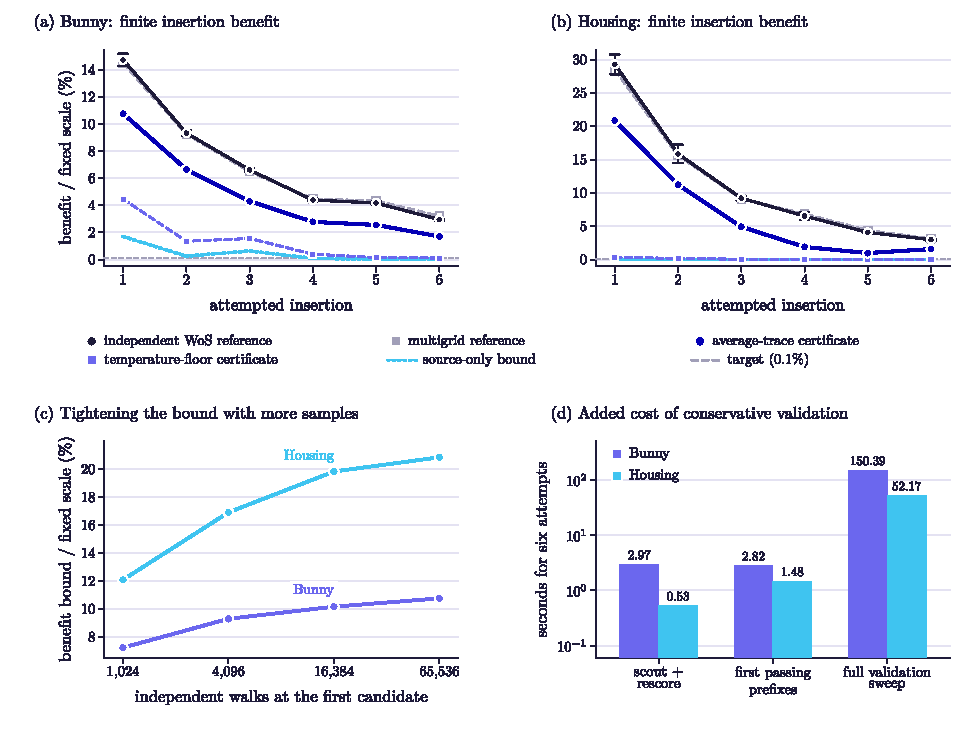
\includegraphics[width=\textwidth]{figures/application-minimum-benefit.pdf}
 \caption{\textbf{A finite benefit bound that can be evaluated before insertion.}
 (a,b) The average-trace certificate is tighter than the temperature-floor
 certificate and source-only bound on the same proposed cavities. Separate
 WoS and multigrid evaluations estimate the actual benefit; error bars show
 one spatial-block standard error for WoS. Percent axes use fixed scales
 $0.002$ (Bunny) and $0.015$ (housing), not certified baseline objectives.
 The dashed horizontal line marks the primary $0.1\%$-of-scale target.
 (c) Larger validation batches tighten the first candidate's bound.
 (d) Complete six-attempt kernel costs, with recorded first-passing prefixes
 shown separately from the full diagnostic actually executed. The bounds
 assume the stated conditional sampling laws and valid input geometry;
 numerical guard audits are reported separately.}
 \label{fig:applicationvalidation}
\end{figure}

\FloatBarrier
\section{Deterministic PDE and Capacity Proofs}
\label{app:deterministic}

This appendix proves \cref{thm:capacityscale,thm:localtd} without importing a
small-hole expansion.  Constants denoted by $C$ may change from line to line,
but are independent of $z\in Z$ and sufficiently small $\eps$.  We write
$K=K_{\eps,z}$, $\Omega_\eps=\Omega_{\eps,z}$,
$q_\eps=q_{\eps,z}$, and $\rho_\eps=\rho_z(\eps)$ when no confusion can
arise.  The background facts used below---trace and compact embedding,
Lax--Milgram, quasi-continuous representatives, positive distributions, and
local Green-kernel bounds---are standard results of Sobolev and elliptic
potential theory~\cite{evans2010pde,adams1996function,gilbarg2001elliptic}; all
problem-specific consequences are derived explicitly.

\subsection{Why regular shape calculus cannot nucleate the cavity}
\label{app:notshapepath}

\begin{proposition}[Cavity nucleation is not a regular shape path]
\label{prop:notshapepath}
Assume additionally that $\partial\Omega$ and $\partial B$ are connected.
Let $V\in C^1_c(\R^d;\R^d)$ and
$T_t=\operatorname{Id}+tV$.  For all sufficiently small $|t|$, $T_t$ is a
$C^1$ diffeomorphism, $T_t(\Omega)$ is diffeomorphic to $\Omega$, and
$\partial T_t(\Omega)=T_t(\partial\Omega)$ is connected.  Hence no such
regular perturbation satisfies
\begin{equation}
 T_t(\Omega)=\Omega\setminus\overline{(z+\eps B)}
 \label{eq:noshapepath}
\end{equation}
for any $\eps>0$ with $z+\eps\overline B\Subset\Omega$, because the right-hand
side has the two disjoint boundary components $\partial\Omega$ and
$z+\eps\partial B$.  Consequently \cref{eq:tddefinition} is not a directional
shape derivative along a regular deformation of the unperforated domain.
\end{proposition}

\begin{proof}[Proof of \cref{prop:notshapepath}]
We separate the analytic and topological parts.

\textbf{Step 1: $T_t$ is a local diffeomorphism for small $t$.}
Because $V\in C^1_c(\R^d;\R^d)$, the quantity
$L:=\|DV\|_{L^\infty(\R^d)}$ is finite.  Choose $|t|L<1$.  Then
\begin{equation}
 DT_t(x)=I+tDV(x)
\end{equation}
is invertible at every $x$: indeed,
$\|tDV(x)\|<1$, so the Neumann series
$\sum_{k=0}^{\infty}(-tDV(x))^k$ converges to $DT_t(x)^{-1}$.
The inverse-function theorem therefore makes $T_t$ a local $C^1$
diffeomorphism.

\textbf{Step 2: $T_t$ is globally injective and proper.}
For any $x,y\in\R^d$, the mean-value estimate gives
\begin{align}
 \|T_t(x)-T_t(y)\|
 &\ge \|x-y\|-|t|\,\|V(x)-V(y)\|\\
 &\ge (1-|t|L)\|x-y\|.
 \label{eq:bilipschitzlower}
\end{align}
Thus $T_t(x)=T_t(y)$ implies $x=y$.  Since $V$ has compact support,
$T_t(x)=x$ outside a compact set; hence $T_t$ is proper.  A proper injective
local diffeomorphism has open and closed image in connected $\R^d$, so its
image is all of $\R^d$.  Therefore $T_t$ is a global $C^1$ diffeomorphism.

\textbf{Step 3: a diffeomorphism preserves the boundary.}
A homeomorphism preserves closure and interior.  Hence
\begin{align}
 \partial T_t(\Omega)
 &=\overline{T_t(\Omega)}\setminus\operatorname{int}T_t(\Omega)\\
 &=T_t(\overline\Omega)\setminus T_t(\operatorname{int}\Omega)
 =T_t(\partial\Omega).
 \label{eq:boundarymapped}
\end{align}
Because $\partial\Omega$ is connected and $T_t$ is continuous,
$T_t(\partial\Omega)$ is connected.

\textbf{Step 4: an interior cavity creates a second boundary component.}
Put $K_{\eps,z}=z+\eps\overline B\Subset\Omega$ and
$\Omega_{\eps,z}=\Omega\setminus K_{\eps,z}$.  Positive separation of
$K_{\eps,z}$ and $\partial\Omega$ implies
\begin{equation}
 \partial\Omega_{\eps,z}
 =\partial\Omega\,\dot\cup\,(z+\eps\partial B).
 \label{eq:perforatedboundary}
\end{equation}
Both sets are nonempty, closed in the relative boundary, and separated by a
positive distance.  Since each is connected by assumption, they are exactly
two distinct connected components.  Therefore
$\partial\Omega_{\eps,z}$ is disconnected.

\textbf{Step 5: contradiction.}
If \cref{eq:noshapepath} held, \cref{eq:boundarymapped} would make the boundary
of its left-hand side connected, whereas \cref{eq:perforatedboundary} makes
the boundary of its right-hand side disconnected.  This is impossible.
Regular Eulerian shape calculus differentiates $J(T_t(\Omega))$ at $t=0$;
the perforated family does not lie on any such path.  Its capacity-normalized
limit is therefore a genuinely singular topological derivative rather than a
directional derivative at the original unperforated domain.  The argument
does not rule out additional asymptotic analysis of shape derivatives on
domains with pre-existing positive-radius cavities.
\end{proof}

\subsection{Functional-analytic foundation}

Equip $V=H^1_{\Gamma_D}(\Omega)$ with
\begin{equation}
 \|v\|_a^2:=a_\Omega(v,v).
 \label{eq:energynorm}
\end{equation}

\begin{proposition}[Boundedness and coercivity]
\label{prop:coercivity}
There are constants $c_a,C_a>0$ such that for all $v,w\in V$,
\begin{equation}
 |a_\Omega(v,w)|\le C_a\|v\|_{H^1}\|w\|_{H^1},
 \qquad
 a_\Omega(v,v)\ge c_a\|v\|_{H^1}^2.
 \label{eq:coercivity}
\end{equation}
The same coercivity constant applies to every perforated test space after
zero extension across the cavity.
\end{proposition}

\begin{proof}
\textbf{Step 1: boundedness.}
H\"older's inequality and the coefficient bounds give
\begin{align}
 |a_\Omega(v,w)|
 &\le \kappa_+\|\nabla v\|_2\|\nabla w\|_2
   +\|\sigma\|_\infty\|v\|_2\|w\|_2\\
 &\le C_a\|v\|_{H^1}\|w\|_{H^1}.
\end{align}

\textbf{Step 2: a Poincar\'e inequality.}
Because the trace vanishes on a boundary subset of positive
$(d-1)$-dimensional measure, there is $C_P<\infty$ such that
\begin{equation}
 \|v\|_{L^2(\Omega)}\le C_P\|\nabla v\|_{L^2(\Omega)}
 \qquad(v\in V).
 \label{eq:mixedpoincare}
\end{equation}
Indeed, if this failed, a normalized sequence with unit $L^2$ norm and
vanishing gradients would converge in $L^2$ to a nonzero constant; continuity
of the trace would force that constant to vanish on $\Gamma_D$, a
contradiction.

\textbf{Step 3: coercivity.}
Since $\sigma\ge0$ and $\kappa\ge\kappa_-$,
\begin{equation}
 a_\Omega(v,v)\ge\kappa_-\|\nabla v\|_2^2
 \ge\frac{\kappa_-}{1+C_P^2}\|v\|_{H^1}^2.
\end{equation}
If $v$ is a perforated-domain test function, its zero extension across $K$
belongs to $V$ because its trace on $\partial K$ is zero.  Applying the same
inequality to that extension proves the final assertion.
\end{proof}

\begin{proposition}[Well-posed state, adjoint, and perforated state]
\label{prop:wellposedness}
The weak problems in \cref{eq:stateweak,eq:adjointweak} have unique solutions.
For every sufficiently small $\eps$, the perforated state with trace $g$ on
$\Gamma_D$ and $h_z$ on $\partial K$ also exists uniquely.  Its extension by
$h_z$ inside $K$ belongs to $H^1(\Omega)$.
\end{proposition}

\begin{proof}
\textbf{Step 1: the state.}
Choose the fixed lift $g\in H^1(\Omega)$ and write $u=g+u_0$ with $u_0\in V$.
Then
\begin{equation}
 a_\Omega(u_0,v)=\ell_\Omega(v)-a_\Omega(g,v)
 \qquad(v\in V).
\end{equation}
The right side is a bounded linear functional.  Boundedness and coercivity
from \cref{prop:coercivity} allow the Lax--Milgram theorem to give a unique
$u_0$, hence a unique $u$.

\textbf{Step 2: the adjoint.}
Because $j'(u)$ is bounded on $L^2(\Omega)$, its restriction to $V$ is bounded
by the continuous embedding $V\hookrightarrow L^2$.  Another application of
Lax--Milgram gives a unique $p\in V$ satisfying
\cref{eq:adjointweak}.

\textbf{Step 3: the perforated state.}
Define
\begin{equation}
 V_\eps:=\{v\in H^1(\Omega_\eps):
 \operatorname{Tr}v=0\text{ on }\Gamma_D\cup\partial K\}.
\end{equation}
Since $K\Subset\Omega$, a smooth cutoff supplies an $H^1(\Omega_\eps)$ lift
with outer trace $g$ and inner trace $h_z$.  Subtracting that lift reduces the
problem to $V_\eps$.  The zero-extension argument in
\cref{prop:coercivity} supplies uniform coercivity, so Lax--Milgram again gives
existence and uniqueness.

\textbf{Step 4: extension across the cavity.}
The trace of $u_{\eps,z}$ on $\partial K$ equals the trace of the constant
function $h_z$ inside $K$.  The Sobolev gluing lemma therefore shows that the
piecewise definition $\widetilde u_{\eps,z}=u_{\eps,z}$ on $\Omega_\eps$ and
$\widetilde u_{\eps,z}=h_z$ on $K$ belongs to $H^1(\Omega)$.
\end{proof}

\subsection{Equilibrium potential and capacitary measure}

Let
\begin{equation}
 \mathcal A_{\eps,z}:=\{v\in V:\widetilde v\ge1
 \text{ quasi-everywhere on }K_{\eps,z}\}.
\end{equation}

\begin{lemma}[Equilibrium potential]
\label{lem:equilibrium}
The class $\mathcal A_{\eps,z}$ is nonempty, closed, and convex.  It has a
unique minimum-energy element $q_\eps$.  This minimizer satisfies
\begin{align}
 0\le q_\eps&\le1\quad\text{quasi-everywhere},\notag\\
 q_\eps&=1\quad\text{quasi-everywhere on }K,
 \label{eq:qrange}\\
 a_\Omega(q_\eps,\varphi)&=0
 \quad\text{if }\varphi\in V
 \text{ and }\widetilde\varphi=0\text{ q.e. on }K.
 \label{eq:qharmonic}
\end{align}
\end{lemma}

\begin{proof}
\textbf{Step 1: nonemptiness and convexity.}
Because $K\Subset\Omega$, a compactly supported smooth cutoff equal to one on
a neighborhood of $K$ belongs to $\mathcal A_{\eps,z}$.  Convexity is
immediate from the pointwise inequality.

\textbf{Step 2: weak closedness.}
Let $v_n\in\mathcal A_{\eps,z}$ converge weakly in $V$ to $v$.  Mazur's lemma
provides convex combinations of tails of $(v_n)$ that converge strongly to
$v$ in $V$.  A subsequence of a strongly $H^1$-convergent sequence converges
quasi-everywhere.  Every convex combination remains at least one
quasi-everywhere on $K$, hence so does $v$.  Thus $v\in\mathcal A_{\eps,z}$.

\textbf{Step 3: existence and uniqueness.}
A minimizing sequence is bounded by coercivity.  Weak compactness and the
preceding closure give a weak limit in $\mathcal A_{\eps,z}$; weak lower
semicontinuity of the squared Hilbert norm gives a minimizer.  Strict
convexity of $a_\Omega(v,v)$ on $V$ gives uniqueness.

\textbf{Step 4: truncation.}
The map $T(s)=\min(1,\max(0,s))$ is one-Lipschitz, satisfies
$|T(s)|\le|s|$, and preserves the constraint on $K$.  The Sobolev chain rule
therefore gives
\begin{equation}
 a_\Omega(T(q_\eps),T(q_\eps))
 \le a_\Omega(q_\eps,q_\eps).
\end{equation}
Uniqueness forces $T(q_\eps)=q_\eps$, proving \cref{eq:qrange}.

\textbf{Step 5: harmonicity away from the obstacle.}
If $\widetilde\varphi=0$ quasi-everywhere on $K$, then
$q_\eps+t\varphi$ is admissible for every $t\in\R$.  Differentiating its
quadratic energy at $t=0$ in both signs gives
$a_\Omega(q_\eps,\varphi)=0$.
\end{proof}

\begin{lemma}[Capacitary measure and localization]
\label{lem:capacitymeasure}
There is a finite positive Radon measure $\mu_\eps$ supported on $\overline K$
such that
\begin{equation}
 a_\Omega(q_\eps,v)=\int_{\overline K}\widetilde v\,\mathrm d\mu_\eps
 \quad(v\in V),
 \qquad
 \mu_\eps(\overline K)=\rho_\eps.
 \label{eq:measureidentity}
\end{equation}
Consequently, for every $v\in V\cap C^1(U)$,
\begin{equation}
 |a_\Omega(q_\eps,v)-\rho_\eps v(z)|
 \le \eps R_B\rho_\eps\|\nabla v\|_{L^\infty(U)},
 \label{eq:capacitylocalization}
\end{equation}
where $B\subset B_{R_B}(0)$.
\end{lemma}

\begin{proof}
\textbf{Step 1: positivity.}
For every nonnegative $\varphi\in C_c^\infty(\Omega)$ and $t>0$,
$q_\eps+t\varphi$ is admissible.  Minimality gives
\begin{equation}
 0\le\frac{a(q_\eps+t\varphi,q_\eps+t\varphi)
               -a(q_\eps,q_\eps)}{2t}
 =a(q_\eps,\varphi)+\frac t2a(\varphi,\varphi).
\end{equation}
Letting $t\downarrow0$ yields $a(q_\eps,\varphi)\ge0$.  Thus
$\varphi\mapsto a(q_\eps,\varphi)$ is a positive distribution and hence a
positive Radon measure $\mu_\eps$.

\textbf{Step 2: support.}
By \cref{eq:qharmonic}, this distribution vanishes on every test function
supported in $\Omega\setminus\overline K$.  Therefore
$\operatorname{supp}\mu_\eps\subseteq\overline K$.

\textbf{Step 3: obtain the mass without extending the measure identity.}
Choose $\chi\in C_c^\infty(U)$ with $\chi=1$ on a neighborhood of $K$.
The function $q_\eps-\chi$ belongs to $V$ and vanishes quasi-everywhere
on $K$. Thus \cref{eq:qharmonic}, applied directly in $V$, gives
\[
 \rho_\eps=a(q_\eps,q_\eps)=a(q_\eps,\chi)
 =\int\chi\,d\mu_\eps=\mu_\eps(K).
\]
The integral identity here is used only for the smooth compactly supported
function $\chi$, for which Steps 1--2 already prove it.

\textbf{Step 4: the measure does not charge polar sets.}
For a compact capacity-zero set $F\subset K$, the smooth-cutoff
characterization of Sobolev capacity gives nonnegative
$\eta_n\in C_c^\infty(\Omega)$ that are at least one near $F$ and satisfy
$\|\eta_n\|_a\to0$. This interior characterization agrees with the relative
capacity: multiply admissible approximations by a fixed interior cutoff,
use norm equivalence, and the usual smooth approximation characterization
of Sobolev capacity. Only compact subsets of $K\Subset\Omega$ are needed.
Positivity and the already established smooth-test identity imply
\[
 \mu_\eps(F)\le\int\eta_n\,d\mu_\eps
 =a(q_\eps,\eta_n)
 \le\rho_\eps^{1/2}\|\eta_n\|_a\longrightarrow0.
\]
Inner regularity of the finite Radon measure then proves the same assertion
for every Borel capacity-zero subset of $K$.

\textbf{Step 5: extend locally by an energy bound.}
For $\varphi\in C_c^\infty(\Omega)$, use the smooth nonnegative functions
$T_\delta(\varphi)=\sqrt{\varphi^2+\delta^2}-\delta$.
They have the same compact support, converge to $|\varphi|$, and satisfy
$\|T_\delta(\varphi)\|_a\le\|\varphi\|_a$ by the chain rule and $\sigma\ge0$.
Consequently, dominated convergence on the finite measure space gives
\[
 \int|\varphi|\,d\mu_\eps
 =\lim_{\delta\downarrow0}a(q_\eps,T_\delta(\varphi))
 \le\rho_\eps^{1/2}\|\varphi\|_a.
\]
If smooth compactly supported $\varphi_n$ converge to $w\in H^1_0(\Omega)$,
this inequality makes them Cauchy in $L^1(\mu_\eps)$. A subsequence converges
quasi-everywhere to $\widetilde w$ and, by Step 4, also $\mu_\eps$-almost
everywhere. Its $L^1(\mu_\eps)$ limit is therefore $\widetilde w$.
Passing to the limit in the smooth-test identity proves
$a(q_\eps,w)=\int\widetilde w\,d\mu_\eps$ for $w\in H^1_0(\Omega)$.

\textbf{Step 6: extend to the mixed-boundary space by localization.}
For an arbitrary $v\in V$, $\chi v\in H^1_0(\Omega)$, while
$v-\chi v$ vanishes on $K$. Orthogonality in \cref{eq:qharmonic} and Step 5 give
\[
 a(q_\eps,v)=a(q_\eps,\chi v)
 =\int_K\chi\widetilde v\,d\mu_\eps
 =\int_K\widetilde v\,d\mu_\eps.
\]
This avoids assuming that $C_c^\infty(\Omega)$ is dense in $V$, which would
be false when nonzero traces are allowed on $\Gamma_N$.

\textbf{Step 7: localization of a smooth observable.}
For $v\in V\cap C^1(U)$, every $x\in K$ obeys $|x-z|\le\eps R_B$.
Using the mass from Step 3,
\begin{align}
 |a(q_\eps,v)-\rho_\eps v(z)|
 &=\left|\int_K(v(x)-v(z))\,d\mu_\eps(x)\right|\\
 &\le\eps R_B\|\nabla v\|_{L^\infty(U)}\rho_\eps.
\end{align}
This proves \cref{eq:capacitylocalization} and completes the extension argument.
\end{proof}

\subsection{Capacity scale}

\begin{proof}[Proof of \cref{thm:capacityscale}]
Existence and uniqueness follow from \cref{lem:equilibrium}; coercivity and
the fact that $K$ contains a ball imply $\rho_\eps>0$.

\paragraph{The three-dimensional upper bound.}
Let $P_B$ be the Newtonian equilibrium potential of $B$:
$P_B=1$ quasi-everywhere on $B$, $P_B\to0$ at infinity, and
\begin{equation}
 \int_{\R^3}|\nabla P_B|^2\,\mathrm dy=\operatorname{cap}(B).
 \label{eq:newtoniancapacity}
\end{equation}
Choose a fixed cutoff $\chi\in C_c^\infty(\Omega)$ that equals one on a
neighborhood of $Z$.  The function
\begin{equation}
 v_{\eps,z}(x):=\chi(x)P_B((x-z)/\eps)
\end{equation}
is admissible for all sufficiently small $\eps$.  After the change of
variables $x=z+\eps y$, local uniform convergence
$\kappa(z+\eps y)\to\kappa(z)$ and the finite energy of $P_B$ yield
\begin{equation}
 \int_\Omega\kappa|\nabla v_{\eps,z}|^2\,\mathrm dx
 =\eps\kappa(z)\operatorname{cap}(B)+o(\eps).
 \label{eq:capupper3dgrad}
\end{equation}
The terms in which the gradient hits $\chi$ occur a fixed positive distance
from $z$, where $P_B((x-z)/\eps)=O(\eps)$; they are $O(\eps^2)$.  Likewise
$\int\sigma v_{\eps,z}^2=O(\eps^2)=o(\eps)$.  Minimality of $q_\eps$ gives
\begin{equation}
 \limsup_{\eps\downarrow0}\frac{\rho_\eps}{\eps}
 \le\kappa(z)\operatorname{cap}(B).
 \label{eq:capupper3d}
\end{equation}

\paragraph{The three-dimensional lower bound.}
Define $Q_\eps(y)=q_\eps(z+\eps y)$ on
$(\Omega-z)/\eps$. The upper bound makes $\int|\nabla Q_\eps|^2$ uniformly bounded. Moreover, Sobolev embedding and coercivity on the fixed domain give $\|q_\eps\|_{L^6(\Omega)}\le C\rho_\eps^{1/2}=O(\eps^{1/2})$. Rescaling yields a uniform $L^6$ bound for $Q_\eps$. Local weak compactness and a diagonal subsequence therefore give a limit $Q$ with $Q\in L^6(\R^3)$ and $\nabla Q\in L^2(\R^3)$, hence $Q\in D^{1,2}(\R^3)$. The cavity constraint passes to the limit by weak closedness on any fixed ball containing $B$, so $Q\ge1$ quasi-everywhere on $B$.  For every fixed $R$,
uniform convergence of the coefficient and weak lower semicontinuity give
\begin{align}
 \liminf_{\eps\downarrow0}\frac{\rho_\eps}{\eps}
 &\ge\liminf_{\eps\downarrow0}
 \int_{B_R}\kappa(z+\eps y)|\nabla Q_\eps|^2\,\mathrm dy\\
 &\ge\kappa(z)\int_{B_R}|\nabla Q|^2\,\mathrm dy.
\end{align}
Letting $R\to\infty$ and then using the variational definition in
\cref{eq:newtoniancapacity} yields
\begin{equation}
 \liminf_{\eps\downarrow0}\frac{\rho_\eps}{\eps}
 \ge\kappa(z)\operatorname{cap}(B).
 \label{eq:caplower3d}
\end{equation}
Together, \cref{eq:capupper3d,eq:caplower3d} prove the $d=3$ formula.

\paragraph{The two-dimensional upper bound.}
By compactness, choose $r_0>0$ so that
\begin{equation}
 B_{2r_0}(z)\Subset\Omega\qquad\text{for every }z\in Z.
\end{equation}
Let $B\subset B_{R_B}(0)$.  Put
$L_\eps=\log(r_0/(\eps R_B))$ and use the radial competitor
\begin{equation}
 v(r)=
 \begin{cases}
 1,&r\le\eps R_B,\\
 \log(r_0/r)/L_\eps,&\eps R_B<r<r_0,\\
 0,&r\ge r_0.
 \end{cases}
\end{equation}
A direct polar-coordinate calculation gives
\begin{equation}
 \int_{\eps R_B}^{r_0}|v'(r)|^2\,2\pi r\,\mathrm dr
 =\frac{2\pi}{L_\eps}.
 \label{eq:annulusenergy}
\end{equation}
Uniform continuity of $\kappa$ and then $r_0\downarrow0$ show
\begin{equation}
 \limsup_{\eps\downarrow0}
 |\log\eps|\rho_\eps\le2\pi\kappa(z).
 \label{eq:capupper2d}
\end{equation}
The zero-order energy is $O(L_\eps^{-2})+O(\eps^2)$ and therefore does not
alter this limit.

\paragraph{The two-dimensional lower bound.}
Choose $r_B>0$ with $B_{r_B}(0)\subset B$.  Fix $r_0$ as above and let
$\delta>0$ be such that
$\kappa(x)\ge\kappa(z)-\delta$ on $B_{r_0}(z)$.  For an admissible $v$, let
$c$ be its circular mean on $\partial B_{r_0}(z)$.  Applying Cauchy--Schwarz
to the radial derivative of the circular mean gives
\begin{equation}
 \int_{B_{r_0}(z)\setminus B_{\eps r_B}(z)}|\nabla v|^2\,\mathrm dx
 \ge\frac{2\pi(1-c)_+^2}{\log(r_0/(\eps r_B))}.
 \label{eq:annuluslower}
\end{equation}
On the fixed exterior domain $\Omega\setminus B_{r_0}(z)$, the trace theorem,
the Poincar\'e inequality on functions vanishing at $\Gamma_D$, and
\cref{eq:coercivity} give
\begin{equation}
 a_{\Omega\setminus B_{r_0}(z)}(v,v)\ge C_0c^2
 \label{eq:outerresistance}
\end{equation}
with $C_0>0$ uniform on $Z$.  Minimizing the sum of
$A(1-c)_+^2+C_0c^2$, where
$A=2\pi(\kappa(z)-\delta)/\log(r_0/(\eps r_B))$, gives
\begin{equation}
 \rho_\eps\ge\frac{AC_0}{A+C_0}.
\end{equation}
First let $\eps\downarrow0$ and then $\delta\downarrow0$ to obtain
\begin{equation}
 \liminf_{\eps\downarrow0}|\log\eps|\rho_\eps
 \ge2\pi\kappa(z).
 \label{eq:caplower2d}
\end{equation}
This and \cref{eq:capupper2d} prove the $d=2$ formula.

\paragraph{Uniformity and comparison with volume.}
All cutoffs, radii, trace constants, and coefficient moduli can be chosen
uniformly because $Z$ is compactly contained in $\Omega$.  A contradiction
argument applied to any sequence $z_n\in Z$, $\eps_n\downarrow0$ upgrades the
pointwise limits to uniform ones.  Finally,
$\eps^3=o(\eps)$ in $d=3$ and
$\eps^2=o(1/|\log\eps|)$ in $d=2$, proving
$\eps^d=o(\rho_\eps)$.
\end{proof}

\subsection{Potential and corrector estimates}

\begin{lemma}[$L^2$ size of the equilibrium potential]
\label{lem:qLtwo}
For $d\in\{2,3\}$,
\begin{equation}
 \|q_\eps\|_{L^2(\Omega)}\le C\rho_\eps.
 \label{eq:qLtwo}
\end{equation}
\end{lemma}

\begin{proof}
The coercive mixed-boundary operator has a positive Green kernel $G(x,y)$.
For $y$ in the fixed interior neighborhood $U$, its local singularity and
regular part satisfy
\begin{equation}
 0\le G(x,y)\le C
 \begin{cases}
 1+|\log|x-y||,&d=2,\\
 |x-y|^{-1}+1,&d=3.
 \end{cases}
 \label{eq:greenbound}
\end{equation}
These bounds follow by freezing the uniformly elliptic principal coefficient,
using the Laplace fundamental solution as a local parametrix, and applying the
maximum principle plus interior elliptic estimates to the regular remainder.
Both right sides are square-integrable in $x$ on a bounded domain, uniformly
for $y\in U$; hence
$\sup_{y\in U}\|G(\cdot,y)\|_2\le C_G$.

By \cref{eq:measureidentity}, $q_\eps$ is the unique weak solution of
$Lq_\eps=\mu_\eps$ with homogeneous outer conditions, so
\begin{equation}
 q_\eps(x)=\int_KG(x,y)\,\mathrm d\mu_\eps(y).
\end{equation}
Minkowski's integral inequality and
$\mu_\eps(K)=\rho_\eps$ yield
\begin{equation}
 \|q_\eps\|_2
 \le\int_K\|G(\cdot,y)\|_2\,\mathrm d\mu_\eps(y)
 \le C_G\rho_\eps.
\end{equation}
\end{proof}

\begin{lemma}[State corrector]
\label{lem:statecorrector}
Let $w_\eps:=\widetilde u_{\eps,z}-u$ and define
\begin{equation}
 r_\eps:=w_\eps+(u(z)-h_z)q_\eps.
 \label{eq:correctordefinition}
\end{equation}
Then
\begin{align}
 \|r_\eps\|_a&\le C\eps^{d/2},
 \label{eq:correctorenergy}\\
 |a_\Omega(r_\eps,p)|&\le C\eps^{d/2},
 \label{eq:correctoradjoint}\\
 \|w_\eps\|_{L^2(\Omega)}&\le C\rho_\eps.
 \label{eq:stateLtwo}
\end{align}
In particular, $a_\Omega(r_\eps,p)=o(\rho_\eps)$ uniformly on $Z$.
\end{lemma}

\begin{proof}
\textbf{Step 1: the corrector equation and trace.}
The state equations on $\Omega_\eps$ imply that $w_\eps$ is $a$-harmonic
against every test function vanishing on both the outer Dirichlet boundary and
$\partial K$.  The same is true of $q_\eps$ by
\cref{eq:qharmonic}.  Therefore $r_\eps$ is $a$-harmonic on
$\Omega_\eps$.  On the cavity boundary,
\begin{equation}
 r_\eps=h_z-u+(u(z)-h_z)=u(z)-u.
 \label{eq:correctortrace}
\end{equation}

\textbf{Step 2: a localized lift.}
Choose $R>R_B$ and $\chi\in C_c^\infty(B_{2R}(0))$ with
$\chi=1$ on $B_R(0)$.  For sufficiently small $\eps$, define
\begin{equation}
 \eta_\eps(x):=\chi((x-z)/\eps)(u(z)-u(x)).
\end{equation}
It has the trace in \cref{eq:correctortrace}.  Local $C^1$ regularity gives
$|u(z)-u(x)|\le C\eps$ on its support and
\begin{align}
 |\nabla\eta_\eps|
 &\le\eps^{-1}|\nabla\chi((x-z)/\eps)|
              \cdot|u(z)-u(x)|\notag\\
 &\quad+|\chi((x-z)/\eps)|\cdot|\nabla u(x)|\notag\\
 &\le C.
\end{align}
Because the support has volume $O(\eps^d)$,
\begin{equation}
 a_\Omega(\eta_\eps,\eta_\eps)\le C\eps^d.
 \label{eq:liftenergy}
\end{equation}

\textbf{Step 3: energy minimality.}
On $\Omega_\eps$, both $r_\eps$ and $\eta_\eps$ have the same boundary trace.
Thus $r_\eps-\eta_\eps$ is an admissible homogeneous test function, and
$a_{\Omega_\eps}(r_\eps,r_\eps-\eta_\eps)=0$.  Consequently
\begin{equation}
 a_{\Omega_\eps}(\eta_\eps,\eta_\eps)
 =a_{\Omega_\eps}(r_\eps,r_\eps)
  +a_{\Omega_\eps}(\eta_\eps-r_\eps,\eta_\eps-r_\eps).
\end{equation}
Inside $K$, the extension of $r_\eps$ equals $u(z)-u(x)$ and has energy
$O(\eps^d)$.  Combining this fact with \cref{eq:liftenergy} proves
\cref{eq:correctorenergy}.

\textbf{Step 4: adjoint pairing.}
Cauchy--Schwarz in the energy inner product gives
\begin{equation}
 |a(r_\eps,p)|\le\|r_\eps\|_a\|p\|_a
 \le C\eps^{d/2},
\end{equation}
which is \cref{eq:correctoradjoint}.

\textbf{Step 5: $L^2$ size of the state perturbation.}
From \cref{eq:correctordefinition}, Poincar\'e's inequality, and
\cref{lem:qLtwo},
\begin{align}
 \|w_\eps\|_2
 &\le |u(z)-h_z|\,\|q_\eps\|_2+\|r_\eps\|_2\\
 &\le C\rho_\eps+C\eps^{d/2}.
\end{align}
The capacity scales show $\eps^{d/2}=o(\rho_\eps)$ for $d=2,3$, proving
\cref{eq:stateLtwo}.  The same comparison applied to
\cref{eq:correctoradjoint} proves the final statement.
\end{proof}

\subsection{Objective expansion}

\begin{proof}[Proof of \cref{thm:localtd}]
Fix $z\in Z$ and abbreviate $a_z=u(z)-h_z$.

\textbf{Step 1: Taylor expansion of the state objective.}
By \cref{eq:stateLtwo}, $w_\eps\to0$ in $L^2$.  The integral form of the
second-order Fr\'echet remainder is
\begin{equation}
 j(u+w_\eps)-j(u)-j'(u)[w_\eps]
 =\int_0^1(1-t)j''(u+tw_\eps)[w_\eps,w_\eps]\,\mathrm dt.
\end{equation}
The uniform bound on $j''$ and \cref{eq:stateLtwo} imply
\begin{equation}
 |j(u+w_\eps)-j(u)-j'(u)[w_\eps]|
 \le C\rho_\eps^2.
 \label{eq:objectiveTaylorbound}
\end{equation}

\textbf{Step 2: explicit domain cost.}
The only explicit domain change is
\begin{equation}
 \left|\int_{\Omega_\eps}\psi-\int_\Omega\psi\right|
 =\left|\int_K\psi\right|
 \le\|\psi\|_\infty|B|\eps^d.
 \label{eq:domaincostbound}
\end{equation}

\textbf{Step 3: adjoint substitution.}
The extension $w_\eps$ has zero trace on $\Gamma_D$, hence belongs to $V$.
By \cref{eq:adjointweak,eq:correctordefinition},
\begin{equation}
 j'(u)[w_\eps]
 =a_\Omega(w_\eps,p)
 =-a_z a_\Omega(q_\eps,p)+a_\Omega(r_\eps,p).
 \label{eq:adjointcorrector}
\end{equation}

\textbf{Step 4: localization of the capacitary charge.}
Applying \cref{eq:capacitylocalization} to the locally $C^1$ adjoint gives
\begin{equation}
 a_\Omega(q_\eps,p)
 =\rho_\eps p(z)+e_{\eps,z},
 \qquad |e_{\eps,z}|\le C\eps\rho_\eps.
 \label{eq:adjointlocalization}
\end{equation}
Combining \cref{eq:correctoradjoint,eq:adjointcorrector,eq:adjointlocalization}
yields
\begin{equation}
 j'(u)[w_\eps]
 =-\rho_\eps(u(z)-h_z)p(z)
  +O(\eps\rho_\eps)+O(\eps^{d/2}).
 \label{eq:firstvariationfinal}
\end{equation}

\textbf{Step 5: collect and express the remainder in capacity units.}
Equations \cref{eq:objectiveTaylorbound,eq:domaincostbound,eq:firstvariationfinal}
give
\begin{align}
 &\left|\J(\Omega_{\eps,z})-\J(\Omega)
 +\rho_\eps(u(z)-h_z)p(z)\right|\notag\\
 &\hspace{16mm}\le
 C\left(\rho_\eps^2+\eps\rho_\eps
        +\eps^{d/2}+\eps^d\right).
 \label{eq:rawremainder}
\end{align}
For $d=3$, $\rho_\eps\asymp\eps$, so every term on the right is bounded by
$C\rho_\eps^{3/2}$.  For $d=2$,
$\rho_\eps\asymp1/|\log\eps|$, and the elementary limit
$\eps|\log\eps|^m\to0$ for every fixed $m$ shows that every term is bounded by
$C\rho_\eps^2$.  This proves \cref{eq:quantitativesmallhole} with
$\alpha_3=1/2$ and $\alpha_2=1$.

\textbf{Step 6: identify the derivative.}
Divide \cref{eq:rawremainder} by $\rho_\eps>0$ and let $\eps\downarrow0$.
The normalized remainder vanishes, so the limit in
\cref{eq:tddefinition} exists and equals
$-(u(z)-h_z)p(z)$.  Every constant above is uniform on $Z$, proving uniform
convergence and \cref{eq:localproduct}.
\end{proof}
\section{Cross-Fitted Estimator Proofs}
\label{app:ustat}

Fix a candidate $z$.  Write
\begin{equation}
 A_i:=U_i-h_z,\qquad B_i:=P_i,
 \qquad \mu_A:=\E A_i,\quad\mu_B:=\E B_i,
\end{equation}
and $X_i=(A_i,B_i)$.  Under the exact-oracle assumption,
$\theta:=-\mu_A\mu_B=\DT(z)$.

\subsection{Algebra and unbiasedness}

\begin{lemma}[Linear-time identity]
\label{lem:lineartime}
For every $N\ge2$,
\begin{equation}
 \sum_{i\ne j}A_iB_j
 =\left(\sum_{i=1}^NA_i\right)
  \left(\sum_{j=1}^NB_j\right)
  -\sum_{i=1}^NA_iB_i.
 \label{eq:lineartimeproof}
\end{equation}
\end{lemma}

\begin{proof}
Distributivity gives
$(\sum_iA_i)(\sum_jB_j)=\sum_{i,j}A_iB_j$.  The index set of this double sum
is the disjoint union of the diagonal $\{i=j\}$ and the off-diagonal
$\{i\ne j\}$.  Subtracting the diagonal proves the identity.  Thus the
estimator needs three scalar sums and $O(N)$ arithmetic.
\end{proof}

\begin{proof}[Proof of \cref{thm:unbiased}]
\textbf{Step 1: factor only across different sample pairs.}
For $i\ne j$, $X_i$ and $X_j$ are independent.  Therefore $A_i$ and $B_j$ are
independent even though $A_i$ and $B_i$ need not be, and
\begin{equation}
 \E[-A_iB_j]=-(\E A_i)(\E B_j)=-\mu_A\mu_B=\theta.
 \label{eq:crossmean}
\end{equation}

\textbf{Step 2: average the ordered terms.}
There are exactly $N(N-1)$ ordered pairs $(i,j)$ with $i\ne j$.  Linearity of
expectation and \cref{eq:crossmean} give
\begin{equation}
 \E\widehat{\DT}_N
 =\frac{1}{N(N-1)}\sum_{i\ne j}\theta=\theta.
\end{equation}
Finally, \cref{eq:oraclemeans,eq:localproduct} imply
$\theta=-(u(z)-h_z)p(z)=\DT(z)$.  At no point was
$\E[A_iB_i]$ factored, so within-pair dependence is unrestricted.
\end{proof}

\subsection{Exact variance decomposition}

Let $A_i^\circ=A_i-\mu_A$ and $B_i^\circ=B_i-\mu_B$.  Recall the symmetric
kernel
\begin{equation}
 H(X_i,X_j)=-\frac12(A_iB_j+A_jB_i),
\end{equation}
for which
\begin{equation}
 \widehat{\DT}_N
 =\binom N2^{-1}\sum_{1\le i<j\le N}H(X_i,X_j).
 \label{eq:ustatunordered}
\end{equation}

\begin{lemma}[Hoeffding projections]
\label{lem:projections}
The first-order and degenerate projections are
\begin{align}
 h_1(X_i)
 &:=-\frac12\left(\mu_BA_i^\circ+\mu_AB_i^\circ\right),
 \label{eq:hprojectionone}\\
 h_2(X_i,X_j)
 &:=-\frac12\left(A_i^\circ B_j^\circ
                  +A_j^\circ B_i^\circ\right).
 \label{eq:hprojectiontwo}
\end{align}
They obey
\begin{align}
 \E h_1(X_i)&=0,\notag\\
 \E[h_2(X_i,X_j)\mid X_i]&=0,\notag\\
 \E[h_2(X_i,X_j)\mid X_j]&=0.
 \label{eq:degeneracy}
\end{align}
\end{lemma}

\begin{proof}
Because $X_j$ is independent of $X_i$,
\begin{align}
 \E[H(X_i,X_j)\mid X_i]
 &=-\frac12(A_i\mu_B+B_i\mu_A).
\end{align}
Subtracting $\theta=-\mu_A\mu_B$ and collecting centered terms gives
\cref{eq:hprojectionone}.  Next expand
\begin{align}
 H(X_i,X_j)
 &=-\mu_A\mu_B
 -\frac12\{\mu_B(A_i^\circ+A_j^\circ)
            +\mu_A(B_i^\circ+B_j^\circ)\}\notag\\
 &\quad-\frac12(A_i^\circ B_j^\circ+A_j^\circ B_i^\circ).
\end{align}
Subtracting $\theta+h_1(X_i)+h_1(X_j)$ proves
\cref{eq:hprojectiontwo}.  Centering and independence across $i\ne j$ give
all three identities in \cref{eq:degeneracy}.
\end{proof}

\begin{proof}[Proof of \cref{thm:variance}]
\textbf{Step 1: decompose the U-statistic.}
Substitute
$H=\theta+h_1(X_i)+h_1(X_j)+h_2(X_i,X_j)$ into
\cref{eq:ustatunordered}.  Every $h_1(X_i)$ appears in $N-1$ unordered pairs,
and $\binom N2=N(N-1)/2$, hence
\begin{equation}
 \widehat{\DT}_N-\theta
 =\frac2N\sum_{i=1}^Nh_1(X_i)
 +\binom N2^{-1}\sum_{i<j}h_2(X_i,X_j).
 \label{eq:hoeffdingdecomposition}
\end{equation}

\textbf{Step 2: prove orthogonality.}
For any $k$ and pair $i<j$, the covariance
$\E[h_1(X_k)h_2(X_i,X_j)]$ is zero.  If $k$ is distinct from both indices,
independence and centering suffice.  If $k=i$, condition on $X_i$ and use
$\E[h_2\mid X_i]=0$; the case $k=j$ is identical.

Two different degenerate terms are also uncorrelated.  Disjoint pairs are
independent.  If $(i,j)$ and $(i,k)$ share one index, then conditioning on
$X_i$ and using independence of $X_j,X_k$ gives zero by degeneracy.  Thus only
identical unordered pairs contribute to the variance of the second sum.

\textbf{Step 3: take variances.}
With $\zeta_1=\Var(h_1(X_1))$ and
$\zeta_2=\Var(h_2(X_1,X_2))$, orthogonality gives
\begin{align}
 \Var(\widehat{\DT}_N)
 &=\frac{4}{N^2}N\zeta_1
 +\binom N2^{-2}\binom N2\zeta_2\\
 &=\frac4N\zeta_1+\frac{2}{N(N-1)}\zeta_2.
 \label{eq:variancefromprojection}
\end{align}

\textbf{Step 4: compute $\zeta_1$.}
Squaring \cref{eq:hprojectionone} and taking expectations gives
\begin{equation}
 \zeta_1=\frac14\left(
 \mu_B^2\Var A+\mu_A^2\Var B
 +2\mu_A\mu_B\Cov(A,B)\right),
\end{equation}
which is \cref{eq:zetaone}.

\textbf{Step 5: compute $\zeta_2$.}
Let $c_{AB}=\E[A_1^\circ B_1^\circ]$.  From
\cref{eq:hprojectiontwo}, independence across sample pairs yields
\begin{align}
 \E h_2^2
 &=\frac14\E\left[
 (A_1^\circ B_2^\circ)^2+(A_2^\circ B_1^\circ)^2
 +2A_1^\circ B_1^\circ A_2^\circ B_2^\circ\right]\\
 &=\frac14\left(2\Var A\,\Var B+2c_{AB}^2\right),
\end{align}
which is \cref{eq:zetatwo}.  The second-moment assumptions make all quantities
finite.  Since $A,B$, and $H$ are evaluated on the unperforated domain, no
$\eps$ occurs anywhere in \cref{eq:variancefromprojection}.
\end{proof}

\subsection{Finite-sample concentration}

\begin{proof}[Proof of \cref{thm:concentration}]
Let $m=\lfloor N/2\rfloor$ and let $\Pi$ be a uniformly random permutation of
$\{1,\ldots,N\}$, independent of the data.  Define the disjoint-pair average
\begin{equation}
 V_\Pi:=\frac1m\sum_{k=1}^m
 H(X_{\Pi(2k-1)},X_{\Pi(2k)}).
 \label{eq:permutationaverage}
\end{equation}

\textbf{Step 1: recover the U-statistic by averaging pairings.}
A fixed unordered pair $\{i,j\}$ is selected in one of the $m$ slots with
probability $2m/[N(N-1)]$.  Its coefficient in
$\E_\Pi[V_\Pi\mid X_1,\ldots,X_N]$ is therefore
\begin{equation}
 \frac1m\frac{2m}{N(N-1)}=\binom N2^{-1}.
\end{equation}
Using \cref{eq:ustatunordered},
\begin{equation}
 \E_\Pi[V_\Pi\mid X_1,\ldots,X_N]=\widehat{\DT}_N.
 \label{eq:pairingidentity}
\end{equation}

\textbf{Step 2: bound the moment-generating function.}
For every $\lambda>0$, convexity of the exponential and
\cref{eq:pairingidentity} give
\begin{align}
 \E\exp\{\lambda(\widehat{\DT}_N-\theta)\}
 &\le\E\E_\Pi\exp\{\lambda(V_\Pi-\theta)\}.
 \label{eq:mgfjensen}
\end{align}
Conditional on a fixed permutation, the $m$ kernel values in
\cref{eq:permutationaverage} use disjoint independent sample pairs.  Each has
mean $\theta$ and lies in $[-M,M]$ because
$|A_i|\le M_U$ and $|B_i|\le M_P$.  Hoeffding's lemma (derived explicitly for a bounded interval in Step 3 of the proof of \cref{prop:onesidedwos}) therefore gives
\begin{equation}
 \E\exp\{\lambda(V_\Pi-\theta)\}
 \le\exp\left(\frac{\lambda^2M^2}{2m}\right).
 \label{eq:mgfhoeffding}
\end{equation}

\textbf{Step 3: Chernoff optimization.}
Markov's inequality and \cref{eq:mgfhoeffding} imply
\begin{equation}
 \Prob(\widehat{\DT}_N-\theta\ge t)
 \le\exp\left(-\lambda t+\frac{\lambda^2M^2}{2m}\right).
\end{equation}
The minimizing value is $\lambda=mt/M^2$.  Substitution produces
\begin{equation}
 \exp\!\left(-\frac{mt^2}{2M^2}\right).
\end{equation}
Applying the same argument to
$-\widehat{\DT}_N$ and adding the two tail probabilities proves
\cref{eq:hoeffdingtail}.

\textbf{Step 4: invert the tail and cover multiple candidates.}
Setting the right side of \cref{eq:hoeffdingtail} equal to $\delta$ gives
\cref{eq:hoeffdingradius}.  For candidate events $F_1,\ldots,F_K$, each with
failure probability at most $\delta/K$, Boole's inequality gives
$\Prob(\cup_kF_k)\le\sum_k\Prob(F_k)\le\delta$.  This argument never assumes
independence across candidate locations.
\end{proof}

\subsection{Marginal bias propagation}

\begin{proof}[Proof of \cref{prop:biaspropagation}]
Put $\bar u=\E U=u+e_U$ and $\bar p=\E P=p+e_P$, where
$|e_U|\le\beta_U$ and $|e_P|\le\beta_P$.  The same cross-index factorization
as in \cref{eq:crossmean} gives
\begin{equation}
 \E\widehat{\DT}_N=-(\bar u-h_z)\bar p.
\end{equation}
Subtracting $\DT=-(u-h_z)p$ and expanding yields the exact identity
\begin{equation}
 \E\widehat{\DT}_N-\DT
 =-p e_U-(u-h_z)e_P-e_Ue_P.
\end{equation}
The triangle inequality and the marginal bounds prove
\cref{eq:productbias}.
\end{proof}

\section{Finite-Difference Lower Bound and Complexity}
\label{app:rareevent}

\begin{proof}[Proof of \cref{thm:rarevariance}]
\textbf{Step 1: lower-bound the per-path second moment.}
By \cref{eq:rarezero},
\begin{align}
 \E Y_\eps^2
 &=\E[Y_\eps^2\mathbf 1_{A_\eps}]
 =\Prob(A_\eps)\E[Y_\eps^2\mid A_\eps]\\
 &\ge c_p c_2\rho_z(\eps).
 \label{eq:raresecondmoment}
\end{align}

\textbf{Step 2: control the squared mean.}
By \cref{eq:raremoments},
\begin{equation}
 (\E Y_\eps)^2\le C_1^2\rho_z(\eps)^2.
\end{equation}
If $\rho_z(\eps)\le c_pc_2/(2C_1^2)$, this is at most
$\tfrac12c_pc_2\rho_z(\eps)$.  Subtracting it from
\cref{eq:raresecondmoment} gives
\begin{equation}
 \Var(Y_\eps)\ge\frac12c_pc_2\rho_z(\eps).
 \label{eq:rareperpathvariance}
\end{equation}

\textbf{Step 3: scale the independent sample mean.}
Independence of the $N$ replicates gives
\begin{align}
 \Var(\widehat{\DT}^{\mathrm{FD}}_{N,\eps})
 &=\frac{1}{N\rho_z(\eps)^2}\Var(Y_\eps)\\
 &\ge\frac{c_pc_2}{2N\rho_z(\eps)},
\end{align}
which is \cref{eq:rarevariance}.
\end{proof}

\begin{proof}[Proof of \cref{cor:ranking}]
Apply \cref{eq:hoeffdingradius} to each candidate with failure probability
$\delta/K$.  The common radius is at most $\Delta$ precisely when
\begin{equation}
 M\sqrt{\frac{2\log(2K/\delta)}{\lfloor N/2\rfloor}}
 \le\Delta,
\end{equation}
which rearranges to \cref{eq:directcomplexity}.  The union bound in
\cref{thm:concentration} then gives simultaneous error at most $\Delta$.
For finite differencing, \cref{eq:rarevariance} and the requirement
$\Var(\widehat{\DT}^{\mathrm{FD}}_{N,\eps})\le\Delta^2$ imply
\cref{eq:fdcomplexity} by direct rearrangement.
\end{proof}

\section{Certification and Adaptive-Selection Proofs}
\label{app:certificate}

\begin{proof}[Proof of \cref{thm:certificate}]
Let
\begin{equation}
 E:=\{|\widehat{\DT}_N-\E\widehat{\DT}_N|
          \le r_N(\delta)\}.
\end{equation}
By hypothesis, $\Prob(E)\ge1-\delta$.

\textbf{Step 1: upper-bound the true derivative on $E$.}
The confidence event and \cref{eq:biasbudget} give
\begin{align}
 \DT(z)
 &\le\E\widehat{\DT}_N(z)
       +b_{\mathrm{term}}+b_{\mathrm{cache}}\\
 &\le\widehat{\DT}_N(z)+r_N(\delta)
       +b_{\mathrm{term}}+b_{\mathrm{cache}}.
 \label{eq:derivativeupperbound}
\end{align}

\textbf{Step 2: insert the deterministic remainder.}
Since $\rho_z(\eps)>0$, the upper side of
\cref{eq:remainderbound} and \cref{eq:derivativeupperbound} imply
\begin{align}
 \J(\Omega_{\eps,z})-\J(\Omega)
 &\le\rho_z(\eps)
       \{\DT(z)+C_z\rho_z(\eps)^\alpha\}\\
 &\le\rho_z(\eps)\{
 \widehat{\DT}_N+r_N+b_{\mathrm{term}}\notag\\[-2pt]
 &\hspace{23mm}{}+b_{\mathrm{cache}}
 +C_z\rho_z(\eps)^\alpha\}.
 \label{eq:certificatebound}
\end{align}
The braced term is negative by \cref{eq:certificate}; hence the objective
change is negative on $E$.  The event has probability at least $1-\delta$.
\end{proof}

\begin{proof}[Proof of \cref{cor:adaptiveradius}]
The event $E$ in the preceding proof is independent of which radius is chosen.
On $E$, \cref{eq:certificatebound} holds simultaneously for every
$\eps\in(0,\eps_0]$ because the remainder assumption is uniform over that
interval.  Therefore it also holds at the measurable random value
$\widehat\eps$.  If \cref{eq:certificate} holds there, the right side is
negative.  Thus failure can occur only on $E^c$, whose probability is at most
$\delta$.  Since one event covers the continuum of radii, no discretization or
union bound is required.
\end{proof}

\begin{proof}[Proof of \cref{prop:freshvalidation}]
Let $B_t$ be the event that round $t$ accepts a non-improving insertion.  The
candidate and radius are $\mathcal F_{t-1}$-measurable.  Conditional on that
history, the proof of \cref{thm:certificate} shows that an accepted insertion
is improving whenever $E_t$ occurs.  Hence
\begin{equation}
 B_t\subseteq E_t^c
 \quad\text{and}\quad
 \Prob(B_t\mid\mathcal F_{t-1})
 \le\Prob(E_t^c\mid\mathcal F_{t-1})\le\delta_t.
\end{equation}
Taking expectations and using the tower property gives
$\Prob(B_t)\le\delta_t$.  Finally, countable subadditivity yields
\begin{equation}
 \Prob\left(\bigcup_{t\ge1}B_t\right)
 \le\sum_{t\ge1}\Prob(B_t)
 \le\sum_{t\ge1}\delta_t,
\end{equation}
which is \cref{eq:sequentialfamilywise}.  No independence between validation
batches is used; only the conditional guarantee is required.
\end{proof}

\section{Source Integration and Connected Refinement}
\label{app:channelimplementation}

\subsection{Poisson source integration}

For completeness, the inhomogeneous three-dimensional Poisson implementation
used in our engineering benchmark samples the Green source term without a
volume grid.  The following identity also fixes the normalization used in our
implementation.

\begin{proposition}[Unbiased source sample on a three-dimensional WoS ball]
\label{prop:greenballsample}
Let $B_R(x)\subset\Omega$, let $\Theta$ be uniform on $\mathbb S^2$, and let
$T$ be independent of $\Theta$ with density $p_T(t)=6t(1-t)$ on $(0,1)$.
For every measurable source $f$ with $\int_{B_R(x)}G_{B_R(x)}(x,y)|f(y)|\,dy<\infty$,
\begin{equation}
 \int_{B_R(x)}G_{B_R(x)}(x,y)f(y)\,dy
 =\frac{R^2}{6}\,\E[f(x+RT\Theta)],
 \label{eq:greenballsample}
\end{equation}
where $G_{B_R(x)}(x,y)=(4\pi)^{-1}
(\|y-x\|^{-1}-R^{-1})$ is the Dirichlet Green kernel evaluated at the ball
center.
\end{proposition}

\begin{proof}
Denote the left-hand side of \cref{eq:greenballsample} by $I_R(x)$ and write
$y=x+r\theta$.  Spherical coordinates, followed by $r=Rt$, give
\begin{align*}
 I_R(x)
 &=\frac1{4\pi}\int_{\mathbb S^2}\int_0^R
   \left(r-\frac{r^2}{R}\right)f(x+r\theta)\,dr\,d\theta\\
 &=\frac{R^2}{4\pi}\int_{\mathbb S^2}\int_0^1
   t(1-t)f(x+Rt\theta)\,dt\,d\theta.
\end{align*}
Uniform $\Theta$ has surface density $(4\pi)^{-1}$ and $T$ has density
$6t(1-t)$; substituting both densities into the expectation on the right of
\cref{eq:greenballsample} gives exactly the last integral.  Hence one draw of
$(T,\Theta)$ yields an unbiased contribution $R^2f(x+RT\Theta)/6$.
\end{proof}

\subsection{Connected-channel parameterization and refinement}

Topology creation need not end with disconnected cavities.  Let
$q=(q_0,\ldots,q_m)\in(\R^3)^{m+1}$ be control points and let a fixed
subdivision matrix $W\in\R^{L\times(m+1)}$ have nonnegative entries and row
sums one.  Dense centers, the removed channel, and the retained domain are
\begin{equation}
 \begin{aligned}
  s_i(q)&=\sum_{j=0}^{m}W_{ij}q_j,\\
  H(q,r)&=\bigcup_{i=1}^{L}\overline B_r(s_i(q)),
  &\Omega(q,r)&=\Omega\setminus H(q,r).
 \end{aligned}
 \label{eq:channelparameterization}
\end{equation}
Every accepted trial must satisfy $\|s_{i+1}-s_i\|<2r$ for all consecutive
centers, checked again after radius recalibration.  Thus the interiors of
successive balls overlap, making both the removed union and its open interior
path connected.  The
topology stage selects two separated terminals and connects them through a
topological-score-weighted candidate graph; Differential WoS then moves the
interior controls while the endpoints remain fixed.
The current housing experiment keeps every ball strictly inside the housing;
its terminals are interior design points.  It therefore demonstrates an
internally connected cavity, not an inlet-to-outlet conduit or a guarantee of
powder evacuation.  In particular, it would remain a void island under the
exterior-reachability definition of Andrade et al.~\cite{andrade2026connectivity}.
The two constraints must not be treated as interchangeable baselines.

Let $\Sigma$ be the union of sphere-intersection seams on $\partial H$.  For
an exposed patch $\Gamma_i$ and offset $\ell>0$, define the admissible part
of that patch by
\begin{equation}
 \Gamma_{i,\ell}^{\mathrm{safe}}=
 \left\{x\in\Gamma_i:
 \operatorname{dist}(x,\Sigma)>\ell,\;
 (x,x-\ell n(x)]\subset\Omega(q,r)\right\}.
 \label{eq:channelsafepatch}
\end{equation}
The Euclidean seam distance is used here; replacing the unit strip width by
any fixed positive multiple changes only constants.

\begin{proposition}[Differential WoS center derivative]
\label{prop:channel-diffwos}
Fix $r>0$ and a regular channel configuration for which the exposed spherical
patches $\Gamma_i\subset\partial H(q,r)$ are $C^2$ away from $\Sigma$.
Assume the piecewise-smooth solution map is shape differentiable under
independent center translations.  Moreover, for every compact probe set
$K\Subset\Omega(q,r)$, assume there are $C_K,\ell_K>0$ such that, for
$0<\ell\le\ell_K$ and $\xi=X_\tau$,
\begin{align}
 \sup_{y\in K}\E_y\!\left[
  \mathbf 1_{\{I(\xi)=i,\,\xi\notin\Gamma_{i,\ell}^{\mathrm{safe}}\}}
  |\partial_nu(\xi)|\right]&\le C_K\ell,
 \label{eq:weightedseamstrip}\\
 \sup_{x\in\Gamma_{i,\ell}^{\mathrm{safe}}}
 \left|\frac{u(x-\ell n(x))}{\ell}+\partial_nu(x)\right|
 &\le C_K\ell.
 \label{eq:safenormaltaylor}
\end{align}
Let $u$ solve
$-\Delta u=f$ in $\Omega(q,r)$ with
zero Dirichlet data.  For $y\in\Omega(q,r)$, let $X_\tau$ be Brownian exit,
$I(X_\tau)$ its exposed-ball index, and $n$ the outward normal of the retained
domain.  If $U_x$ is an unbiased independent WoS estimate of $u(x)$, then
\begin{equation}
 G_{i,\ell}(y)=
 \mathbf 1_{\{I(X_\tau)=i,\,
 X_\tau\in\Gamma_{i,\ell}^{\mathrm{safe}}\}}
 n(X_\tau)\frac{U_{X_\tau-\ell n(X_\tau)}}{\ell}
 \label{eq:diffwoscenterestimator}
\end{equation}
satisfies, uniformly on compact probe sets,
\begin{equation}
 \E G_{i,\ell}(y)=\nabla_{s_i}u(y)+O(\ell)
 \quad\text{as }\ell\downarrow0.
 \label{eq:diffwoscenterbias}
\end{equation}
For any fixed finite set of interior probes, the weighted estimate has $O(\ell)$ bias for the corresponding weighted derivative sum. To assert this rate for compliance $J(q,r)=\int_{\Omega(q,r)}fu\,dx$, additionally assume that differentiation under the domain integral is valid and that, for all sufficiently small $\ell$, the pointwise estimator error is bounded by $\ell C(y)$ with $\int_{\Omega(q,r)}|f(y)|C(y)\,dy<\infty$. A finite probe rule then adds its separate quadrature error.
\end{proposition}

\begin{proposition}[Control chain rule and length tangency]
\label{prop:channel-chainrule}
Suppose $J$ is differentiable with respect to the dense centers at a regular
configuration, and write $G_i=\nabla_{s_i}J$.  Then
\begin{equation}
 \nabla_{q_j}J=\sum_{i=1}^{L}W_{ij}G_i.
 \label{eq:channelchainrule}
\end{equation}
For the centerline length
$\mathcal L(q)=\sum_{j=0}^{m-1}\|q_{j+1}-q_j\|$, let $c$ be its gradient
with the endpoint blocks set to zero.  Given any endpoint-fixed proposal $a$,
define
\begin{equation}
 d=a-c\frac{\langle c,a\rangle}{\|c\|^2}
 \quad(c\ne0),
 \label{eq:lengthprojection}
\end{equation}
and $d=a$ if $c=0$.  Then the endpoints do not move and
$D\mathcal L(q)[d]=0$.  In particular, let $g$ be the objective gradient with
its endpoint blocks set to zero.  Choosing $a=-g$ gives
$DJ(q)[d]=-\|P_{c^\perp}g\|^2\le0$.  Our implementation first
smooths $a$ and therefore relies on fresh line-search validation, rather than
this last inequality, for accepted descent.
\end{proposition}

The radius of every trial is recalibrated on one fixed Sobol set.  If
$Y_1,\ldots,Y_M$ fill a box of volume $V_B$, define
\begin{equation}
 \widehat V_M(q,r)=\frac{V_B}{M}\sum_{k=1}^{M}
 \mathbf 1_{\{Y_k\in\Omega,\;\min_i\|Y_k-s_i(q)\|\le r\}}.
 \label{eq:qmcchannelvolume}
\end{equation}

\begin{proposition}[Discrete equal-volume calibration]
\label{prop:qmc-volume}
Let $k$ be the nearest integer to $MV_\star/V_B$.  If the $k$th and
$(k+1)$st eligible center distances are distinct, choosing $r$ strictly
between them gives exactly $k$ removed samples and
\begin{equation}
 |\widehat V_M(q,r)-V_\star|\le \frac{V_B}{2M}.
 \label{eq:qmcvolumequantum}
\end{equation}
Thus all compared connected channels have the same discrete volume, up to one
predeclared rounding quantum; this is a statement about the fixed QMC measure,
not an exact analytic union-volume formula.
\end{proposition}

\begin{proposition}[Fresh paired shape acceptance]
\label{prop:fresh-shape}
At shape round $t$, condition on the complete history $\mathcal F_{t-1}$,
including the Differential WoS direction and finitely many trial scales.  Let
$\Delta_{t,k}=J(q_{t,k},r_{t,k})-J(q_t,r_t)$, where every $r_{t,k}$ obeys
\cref{eq:qmcchannelvolume}.  Suppose simultaneous upper bounds satisfy
\begin{equation}
 \Prob\!\left(\Delta_{t,k}\le U_{t,k}\ \text{for every }k
 \mid\mathcal F_{t-1}\right)\ge1-\delta_t.
 \label{eq:shapesimultaneouscoverage}
\end{equation}
If a trial is accepted only when its $U_{t,k}<0$, then
\begin{equation}
 \Prob(\text{some accepted shape step is non-improving})
 \le\sum_t\delta_t.
 \label{eq:shapefamilywise}
\end{equation}
The conclusion is independent of bias in the proposed direction: coverage of
the fresh objective difference, not gradient accuracy, certifies acceptance.
\end{proposition}



\section{Connected-Channel Refinement Proofs}
\label{app:channelproofs}

\begin{proof}[Proof of \cref{prop:channel-diffwos}]
We prove the vector identity by testing it against an arbitrary translation
$v\in\R^3$ of ball $i$.

\textbf{Step 1: derive the boundary condition for the shape derivative.}
On the interior of the exposed patch $\Gamma_i$, translation of center $i$
has velocity $V=v$; every other open spherical patch and the outer boundary
have $V=0$.  The proposition's shape-differentiability assumption permits
patchwise trace differentiation; the seam itself is excluded.  Write $u_t$
for the perturbed solution and $\dot u$ for its Eulerian shape derivative at
$t=0$.  Differentiating the
identity $u_t(T_t(x))=0$ for $x\in\Gamma_i$ gives
\begin{equation}
 \dot u(x)+\nabla u(x)\cdot V(x)=0.
 \label{eq:channelmaterialboundary}
\end{equation}
The trace of $u$ is constant on $\Gamma_i$, so its tangential gradient
vanishes there.  Hence $\nabla u=(\partial_nu)n$ and
\begin{equation}
 \dot u=-(n\cdot v)\partial_nu\quad\text{on }\Gamma_i.
 \label{eq:channelshapecondition}
\end{equation}
The source $f$ and the outer boundary are fixed.  Differentiating the weak
Poisson equation with test functions compactly supported in the current
domain therefore gives
\begin{equation}
 -\Delta\dot u=0\quad\text{in }\Omega(q,r),
 \label{eq:channelharmonicderivative}
\end{equation}
with zero trace on all stationary Dirichlet patches.  Equations
\cref{eq:channelshapecondition,eq:channelharmonicderivative} are the standard
differential boundary-value problem, here obtained directly from the moving
trace.

\textbf{Step 2: approximate the normal derivative on the safe patch.}
For $x\in\Gamma_{i,\ell}^{\mathrm{safe}}$, the segment in
\cref{eq:channelsafepatch} lies in the retained domain.  Whenever a uniform
$C^2$ extension is available, Taylor's theorem along this segment and
$u(x)=0$ give
\begin{align}
 u(x-\ell n)
 &=u(x)-\ell\partial_nu(x)
   +\frac{\ell^2}{2}
     n^T\nabla^2u(x-\theta\ell n)n \\
 &=-\ell\partial_nu(x)+O(\ell^2),
 \label{eq:backwardnormaltaylor}
\end{align}
for some $\theta\in(0,1)$.  Uniform $C^2$ bounds on the regular exposed
patches imply
\begin{equation}
 -\partial_nu(x)=\frac{u(x-\ell n(x))}{\ell}+O(\ell)
 \label{eq:backwardnormalderivative}
\end{equation}
there.  In the proposition we use the explicitly stated uniform version
\cref{eq:safenormaltaylor}; this separates the needed analytic estimate from
the merely qualitative fact that $\Sigma$ has zero harmonic measure.
Combining
\cref{eq:channelshapecondition,eq:backwardnormalderivative} yields
\begin{equation}
 \dot u(x)=(n(x)\cdot v)
 \frac{u(x-\ell n(x))}{\ell}+O(\ell\|v\|).
 \label{eq:offsetboundarydata}
\end{equation}

\textbf{Step 3: truncate the harmonic exit representation.}
Let $X_\tau$ denote Brownian exit from $\Omega(q,r)$, and abbreviate
$\xi=X_\tau$ and $n_\tau=n(X_\tau)$.  The harmonic representation of
\cref{eq:channelharmonicderivative} first gives the exact identity
\begin{align}
 D_{s_i}u(y)[v]
 &=\E_y\!\left[
   \mathbf 1_{\{I(\xi)=i\}}
   \bigl(-(n_\tau\cdot v)\partial_nu(\xi)\bigr)\right].
 \label{eq:exactharmonicshaperepresentation}
\end{align}
Write $S_{i,\ell}=\{I(\xi)=i,\,
\xi\in\Gamma_{i,\ell}^{\mathrm{safe}}\}$.  On $S_{i,\ell}$,
\cref{eq:safenormaltaylor} bounds the error made by replacing
$-\partial_nu(\xi)$ with $u(\xi-\ell n_\tau)/\ell$ by $C_K\ell$.
Because harmonic measure has total mass at most one, its contribution is at
most $C_K\ell\|v\|$.  On $\{I(\xi)=i\}\setminus S_{i,\ell}$,
\cref{eq:weightedseamstrip} bounds the discarded part of
\cref{eq:exactharmonicshaperepresentation} by the same order.  Therefore
\begin{align}
 D_{s_i}u(y)[v]
 &=\E_y\!\left[
   \mathbf 1_{S_{i,\ell}}(n_\tau\cdot v)
   \frac{u(\xi-\ell n_\tau)}{\ell}\right]
   +O_K(\ell\|v\|).
 \label{eq:harmonicshaperepresentation}
\end{align}
This is the precise point at which the quantitative strip assumption, rather
than only measure zero of the limiting seam, is required.

\textbf{Step 4: insert the nested WoS estimate.}
Condition on $X_\tau$ on the safe event $S_{i,\ell}$.  By hypothesis,
\begin{equation}
 \E[U_{X_\tau-\ell n(X_\tau)}\mid X_\tau]
 =u(X_\tau-\ell n(X_\tau)).
\end{equation}
Taking iterated expectations in \cref{eq:diffwoscenterestimator} and comparing
with \cref{eq:harmonicshaperepresentation} shows that, for every $v$,
\begin{equation}
 v\cdot\E G_{i,\ell}(y)
 =D_{s_i}u(y)[v]+O(\ell\|v\|).
\end{equation}
Duality in the finite-dimensional space $\R^3$ proves
\cref{eq:diffwoscenterbias}.

\textbf{Step 5: differentiate compliance.}
Reynolds' transport formula gives
\begin{equation}
 D_{s_i}J[v]
 =\int_{\Omega(q,r)}fD_{s_i}u[v]\,dx
  +\int_{\partial\Omega(q,r)}fu(V\cdot n)\,dS.
 \label{eq:channelreynolds}
\end{equation}
The boundary integral vanishes because $u=0$ on every moving and fixed
Dirichlet patch. For a fixed finite interior probe set, compact-set uniformity in \cref{eq:diffwoscenterbias} directly bounds the weighted sum of estimator errors by $O(\ell)$. For the continuum objective, the additional integrable-envelope hypothesis gives
\[
 \begin{aligned}
 &\left\|\int_{\Omega(q,r)}f(y)
 \bigl(\E G_{i,\ell}(y)-\nabla_{s_i}u(y)\bigr)\,dy\right\|\\
 &\qquad\le \ell\int_{\Omega(q,r)}|f(y)|C(y)\,dy.
 \end{aligned}
\]
This proves the continuum rate under the added hypothesis. Compact-set bounds alone would not control probes approaching the boundary. Replacing the integral by a fixed weighted rule adds the separate quadrature error.
\end{proof}

\begin{proof}[Proof of \cref{prop:channel-chainrule}]
\textbf{Step 1: differentiate the dense centers.}
For a control perturbation $\dot q=(\dot q_0,\ldots,\dot q_m)$,
linearity of \cref{eq:channelparameterization} gives
\begin{equation}
 \dot s_i=\sum_{j=0}^{m}W_{ij}\dot q_j.
 \label{eq:densecenterdifferential}
\end{equation}

\textbf{Step 2: apply the ordinary finite-dimensional chain rule.}
At the assumed differentiability point,
\begin{align}
 DJ(q)[\dot q]
 &=\sum_{i=1}^{L}G_i\cdot\dot s_i
 =\sum_{i=1}^{L}G_i\cdot
   \sum_{j=0}^{m}W_{ij}\dot q_j\\
 &=\sum_{j=0}^{m}
   \left(\sum_{i=1}^{L}W_{ij}G_i\right)\cdot\dot q_j.
 \label{eq:channelchainproof}
\end{align}
Since this holds for every $\dot q$, comparison with the definition of the
Euclidean gradient proves \cref{eq:channelchainrule}.

\textbf{Step 3: compute the length gradient.}
Put
$e_j=(q_{j+1}-q_j)/\|q_{j+1}-q_j\|$ and assume no consecutive controls
coincide.  Direct differentiation yields
\begin{equation}
 \begin{aligned}
  \nabla_{q_0}\mathcal L&=-e_0,\\
  \nabla_{q_j}\mathcal L&=e_{j-1}-e_j &&(1\le j<m),\\
  \nabla_{q_m}\mathcal L&=e_{m-1}.
 \end{aligned}
 \label{eq:lengthgradientexplicit}
\end{equation}
For endpoint-fixed directions only the interior blocks contribute, so replacing
the two endpoint blocks by zero gives the vector $c$ in the proposition and
$D\mathcal L(q)[d]=\langle c,d\rangle$.

\textbf{Step 4: verify tangency.}
When $c\ne0$, substitution of \cref{eq:lengthprojection} gives
\begin{equation}
 \langle c,d\rangle
 =\langle c,a\rangle
  -\|c\|^2\frac{\langle c,a\rangle}{\|c\|^2}=0.
\end{equation}
When $c=0$, the same conclusion is immediate.  Both $a$ and $c$ have zero
endpoint blocks, hence so does $d$.

\textbf{Step 5: verify descent for the unsmoothed projected gradient.}
Let $g$ denote $\nabla_qJ$ with its endpoint blocks set to zero and let
$P_{c^\perp}$ be orthogonal projection within that endpoint-fixed subspace.
Choosing $a=-g$ makes $d=-P_{c^\perp}g$.  Therefore
\begin{equation}
 DJ(q)[d]=\langle g,d\rangle
 =-\langle g,P_{c^\perp}g\rangle
 =-\|P_{c^\perp}g\|^2\le0.
\end{equation}
The final equality uses symmetry and idempotence of an orthogonal projection.
No descent assertion follows after an arbitrary smoothing operator; this is
why the implemented smoothed proposal is subjected to fresh evaluation.
\end{proof}

\begin{proof}[Proof of \cref{prop:qmc-volume}]
For each sample define
\begin{equation}
 d_j=\begin{cases}
 \min_i\|Y_j-s_i(q)\|,&Y_j\in\Omega,\\
 +\infty,&Y_j\notin\Omega.
 \end{cases}
\end{equation}
Let $d_{(1)}\le\cdots\le d_{(M)}$ be the order statistics.  If
$d_{(k)}<r<d_{(k+1)}$, exactly the first $k$ indicators in
\cref{eq:qmcchannelvolume} equal one.  Hence
\begin{equation}
 \widehat V_M(q,r)=\frac{kV_B}{M}.
\end{equation}
Since $k$ is a nearest integer to $MV_\star/V_B$,
\begin{equation}
 \left|k-\frac{MV_\star}{V_B}\right|\le\frac12.
\end{equation}
Multiplication by $V_B/M$ proves \cref{eq:qmcvolumequantum}.  The distinctness
assumption prevents ambiguity at the threshold.  If ties occur, a deterministic
tie rule retains a one-quantum bound but need not attain exactly $k$ samples.
\end{proof}

\begin{proof}[Proof of \cref{prop:fresh-shape}]
Let $E_t$ be the simultaneous-coverage event inside
\cref{eq:shapesimultaneouscoverage}, and let $B_t$ be the event that round $t$
accepts a non-improving trial.  On $E_t$, every accepted index $k$ satisfies
\begin{equation}
 \Delta_{t,k}\le U_{t,k}<0.
\end{equation}
Consequently $B_t\subseteq E_t^c$.  Conditional coverage and the tower
property imply
\begin{align}
 \Prob(B_t)
 &=\E[\Prob(B_t\mid\mathcal F_{t-1})]\\
 &\le\E[\Prob(E_t^c\mid\mathcal F_{t-1})]
 \le\delta_t.
\end{align}
Finally, countable subadditivity gives
\begin{equation}
 \Prob\!\left(\bigcup_tB_t\right)
 \le\sum_t\Prob(B_t)\le\sum_t\delta_t,
\end{equation}
which is \cref{eq:shapefamilywise}.  The direction, tested scales, common
random numbers within each paired difference, and deterministic radius
recalibration are all part of the conditioning history.  No correctness
assumption about the Differential WoS proposal is used after that conditioning.
\end{proof}

\section{Reproducibility and Interpretation}
\label{app:checklist}
\label{app:claims}

Detailed protocols appear in \cref{app:experiments,sec:critical}; the count--radius study retains all 72 designs and separates design-seed ranges from conditional evaluation uncertainty. Rendering cuts and scalar smoothing affect only visualization, not the physical domain or reported objectives.

The deterministic capacity expansion uses the analytic hypotheses stated in the main text. Cross-fitted unbiasedness assumes exact marginal oracle means; implemented termination error remains separate. The finite-insertion and shape-acceptance results control erroneous acceptances under their coverage premises, rather than giving posterior probabilities conditional on an accepted design. No application result is presented as a proof that its finite-size, oracle-bias, or interval assumptions hold.

\FloatBarrier
\section{Independent Randomizations for Accelerated Oracles}
\label{app:batchindependence}

\begin{proposition}[Cross-fitting independent accelerated batches]
Fix a candidate, a deterministic geometry, and $R\ge2$. For $r=1,\ldots,R$, independently
generate a full randomized estimator pair $(A_r,B_r)$ with the same law,
means $(a,b)$, and finite second moments.  Paths within a batch can have
arbitrary dependence.  Define
\begin{equation}
 T_R=-\frac{1}{R(R-1)}\sum_{r\ne s}A_rB_s.
\end{equation}
Then $\E T_R=-ab$, and \cref{thm:variance,thm:concentration} apply with batch
count $R$ and the corresponding batch moments and almost-sure bounds.
\end{proposition}
\begin{proof}
For $r\ne s$, the sigma-algebras of the two complete randomizations are
independent.  Thus $A_r$ and $B_s$ are independent and
$\E[A_rB_s]=(\E A_r)(\E B_s)=ab$.  There are $R(R-1)$ ordered pairs;
linearity of expectation gives $\E T_R=-ab$.  Let
$H_{rs}=-(A_rB_s+A_sB_r)/2$.  Then
$T_R=\binom R2^{-1}\sum_{r<s}H_{rs}$, an order-two U-statistic of the
independent batch pairs.  Its first and degenerate second projections are
exactly those in \cref{app:ustat}, with the law of $(A,B)$ now the batch law.
Substitution proves the variance identity.  If $|A_r|\le M_A$ and
$|B_r|\le M_B$, then $|H_{rs}|\le M_AM_B$.  Each disjoint pairing has
$\lfloor R/2\rfloor$ independent kernels; the existing pairing/MGF proof
therefore gives the stated concentration bound.  No independence within a
batch is used at any step.
\end{proof}

\paragraph{What fails if paths are treated as independent.}
For arbitrary dependent pairs with fixed marginal means $a,b$ and integrable
products, direct expansion instead gives
\begin{align}
 \E T_N
 &=-\frac{1}{N(N-1)}\sum_{i\ne j}
       \left(ab+\Cov(A_i,B_j)\right)\\
 &=-ab-\frac{1}{N(N-1)}\sum_{i\ne j}\Cov(A_i,B_j).
 \label{eq:crossindexbias}
\end{align}
Deleting the diagonal removes none of these cross-index covariances.
An exact example uses the unit disk, $u(z)=p(z)=\operatorname{Re}z$, and
$z=0$.  For a random uniform angle $\Theta$, take
$A_j=B_j=\cos(\Theta+2\pi j/N)$, $j=0,\ldots,N-1$, $N\ge3$.
Every sample has the correct harmonic marginal, but
\begin{align}
 \sum_j A_j&=\operatorname{Re}\left(e^{i\Theta}
                    \sum_j e^{2\pi i j/N}\right)=0,\\
 \sum_j A_j^2&=\frac{N}{2}+\frac{1}{2}\operatorname{Re}\left(e^{2i\Theta}
                    \sum_j e^{4\pi i j/N}\right)=\frac N2,\\
 T_N&=-\frac{(\sum_j A_j)^2-\sum_j A_j^2}{N(N-1)}
       \\
    &=\frac{1}{2(N-1)}\ne 0=-u(0)p(0).
\end{align}
Both geometric sums vanish since their ratios are nontrivial $N$th roots
of unity.  Cross-fitting independently randomized batch averages instead
returns zero exactly here.  This counterexample establishes a failure of
the iid formula; it is not a lower bound for general Array-RQMC performance.

\paragraph{A common random cache is a separate independence hazard.}
Suppose the pairs are iid only conditional on a cache $C$, with conditional
means $a(C),b(C)$.  Conditional independence first gives
$\E[T_N\mid C]=-a(C)b(C)$.  Taking expectation again yields
\begin{equation}
 \E T_N=-\E[a(C)]\E[b(C)]-\Cov(a(C),b(C)).
\end{equation}
Thus marginally unbiased field estimators alone do not suffice.  For example,
$A_i=a+C+\xi_i$ and $B_i=b+C+\eta_i$, where $C$ is a symmetric random sign
and all zero-mean noises are independent of it and each other, produce bias
$-1$ for every $N$.  Valid alternatives are independent caches per batch,
conditionally exact fixed means, or a rigorously bounded residual cache bias.

\paragraph{Termination error remains a bias budget.}
The batch result is unbiased for the means of the implemented oracles.
An $\varepsilon$-shell WoS implementation does not thereby become unbiased
for the exact PDE.  On our harmonic disk/square tests, $u,p$ are explicit
smooth polynomials.  At a stopped point $x$ and its boundary projection $y$,
the mean-value inequality gives
$|u(y)-u(x)|\le L_u\varepsilon$ and
$|p(y)-p(x)|\le L_p\varepsilon$, where $L_u,L_p$ bound their gradients.
Optional stopping for bounded harmonic martingales then bounds the marginal
oracle biases by the same quantities.  The product bias is at most
$|a|L_p\varepsilon+|b|L_u\varepsilon+L_uL_p\varepsilon^2$.
If a path cap is exhausted, our benchmark raises an error instead of silently
projecting an interior path.  None of these diagnostics supplies a finite
insertion certificate without the separate small-hole remainder bound.

For the Poisson-compliance disk test, the source is constant and
$u(x)=(1-|x|^2)/4$. The ball mean-value identity is
$u(x)=r^2/4+\E[u(Y)\mid x]$, where $Y$ is uniform on the sphere of radius
$r$ centered at $x$. Iterating and stopping at the shell gives
\begin{equation}
 u(x_0)=\E\!\left[\sum_{k<\tau}\frac{r_k^2}{4}\right]
            +\E[u(X_\tau)].
\end{equation}
This follows first at $\tau\wedge n$, then by monotone convergence for
the nonnegative source sum and bounded convergence for the residual state.
At termination, $1-|X_\tau|\le\varepsilon$, so
$0\le u(X_\tau)=(1-|X_\tau|)(1+|X_\tau|)/4\le\varepsilon/2$.
The implemented source estimator omits this residual and consequently has
marginal bias of magnitude at most $\varepsilon/2$. Since $0\le u\le1/4$
and $p=u$, the general product-bias inequality gives the conservative bound
$\varepsilon/4+\varepsilon^2/4$. Exact constant-source integration therefore
removes source quadrature error, but not shell truncation error.

\section{Oracle-State Shape Benchmark Derivation}
\label{app:shapeoracle}

The controlled shape comparison restricts the admissible domains to ellipses
$\Omega_{a,b}=\{(x,y):x^2/a^2+y^2/b^2<1\}$ with $a,b>0$.
Set $c=[2(a^{-2}+b^{-2})]^{-1}$ and
\begin{equation}
 u_{a,b}(x,y)=c(1-x^2/a^2-y^2/b^2).
\end{equation}
Direct differentiation gives
$-\Delta u_{a,b}=2c(a^{-2}+b^{-2})=1$, while substitution into the ellipse
equation gives zero boundary data.  Uniqueness of the Dirichlet problem
therefore identifies this polynomial as the state.  The fixed target is
$z_d=\max(u_{1,0.65},0)$, and
$J(a,b)=\tfrac12\int_{\Omega_{a,b}}(u_{a,b}-z_d)^2$.
This exact-state setting isolates derivative estimation; it does not reproduce
the neural-state training or boundary metric of Schmidt and
W\"urschmidt~\cite{schmidt2026first}.

\paragraph{Probabilistic pushforward derivative.}
For a smooth admissible velocity $V$, differentiating the Poisson problem at
fixed spatial coordinates gives $-\Delta u'=0$ in $\Omega$ and
$u'=-\nabla u\cdot V$ on $\partial\Omega$.  Feynman--Kac and the transport
formula give, respectively,
\begin{align}
 u'(x)&=-\E_x[\nabla u(Y)\cdot V(Y)],\\
 J'[V]&=\int_\Omega(u-z_d)u'\,dx
          +\frac12\int_{\partial\Omega}z_d^2 V\cdot n\,ds.
\end{align}
All functions are bounded on the compact ellipse closure, so Fubini applies.
If $X$ is uniform on $\Omega$ and $Y$ is a Brownian exit conditional on $X$,
\begin{align}
 J'[V]&=-\pi ab\,\E[(u(X)-z_d(X))\nabla u(Y)\cdot V(Y)]\\
       &\quad+\frac12\int_{\partial\Omega}z_d^2 V\cdot n\,ds.
\end{align}
Splitting the volume integral into the positive and negative parts of
$u-z_d$ recovers the signed-start representation in that work, after its
stated pushforward sign conversion.  Uniform weighted starts estimate the
same integral with a different proposal distribution.
For $V_a=(x/a,0)$ and $V_b=(0,y/b)$, parameterize the boundary by
$y(\theta)=(a\cos\theta,b\sin\theta)$.  Its normal times arclength is
$(b\cos\theta,a\sin\theta)d\theta$, whence
$V_a\cdot n\,ds=b\cos^2\theta\,d\theta$ and
$V_b\cdot n\,ds=a\sin^2\theta\,d\theta$.  These are the two surface terms
integrated by the benchmark.

\paragraph{Independent deterministic check.}
Write $x=a\xi$, $y=b\eta$ on the fixed unit disk.  With
$q=1-\xi^2-\eta^2$, we have $u=cq$ and $dx\,dy=ab\,d\xi\,d\eta$.
Since $\partial_a c=4c^2/a^3$, differentiation at fixed $(\xi,\eta)$ gives
$\partial_a u=4cu/a^3$.  Inside the target ellipse,
$\partial_xz_d=-2c_*x$, where $c_*=[2(1+0.65^{-2})]^{-1}$;
outside it the derivative is zero almost everywhere.  The target is
Lipschitz and its interface has area measure zero, justifying dominated
differentiation of this finite-dimensional pullback.  Therefore
\begin{equation}
 \partial_a J=\int_{\Omega_{a,b}}
 \left[(u-z_d)\left(\frac{4c}{a^3}u-\partial_xz_d\frac{x}{a}\right)
                   +\frac{(u-z_d)^2}{2a}\right]dx\,dy.
\end{equation}
The formula for $\partial_b J$ follows by exchanging the coordinates and
including the target factor $0.65^{-2}$ in $\partial_yz_d$.
We evaluate these integrals by Gauss--Legendre radial and periodic angular
quadrature and independently check central differences of $J$.

\section{Ball-Chain Connectivity and Its Scope}
\label{app:ballchain}
\begin{proposition}[Strict overlap after recalibration]
Let $r>0$ and $s_1,\ldots,s_L\in\R^d$ satisfy
$\|s_{i+1}-s_i\|<2r$ for every $i<L$.  Then
$\bigcup_i B_r(s_i)$ is path connected.  If every closed ball has positive
clearance from $\partial\Omega$ and is contained in $\Omega$, their union
does not meet the exterior boundary, irrespective of this connectedness.
\end{proposition}
\begin{proof}
The midpoint $(s_i+s_{i+1})/2$ is at distance
$\|s_{i+1}-s_i\|/2<r$ from each center, so consecutive open balls intersect.
Every ball is convex and hence path connected.  For any two points in the
union, choose balls containing them; join each point to its center by a
segment, and join the intervening centers through consecutive intersection
midpoints.  The finite concatenation lies inside the union and is a continuous
path.  If each of finitely many closed balls has positive clearance from the
exterior, the minimum of those clearances is positive.  Their union is thus
separated from the exterior.  In particular, strict overlap alone cannot imply
the absence of a sealed void island.  Tangency would only connect closed
balls at a point and is deliberately rejected for the open-channel guarantee.
\end{proof}

\FloatBarrier
\section{Cavity Count, Volume, and Thermal Compliance}
\label{app:cavitybudget}

The following facts explain the budget experiment; they are properties of the
classical ideal Dirichlet cooling model, not new topological-derivative claims.

\begin{proposition}[Monotonicity under additional cooled material removal]
\label{prop:coolingmonotonicity}
Let $\Omega\subset\mathbb R^3$ be bounded and Lipschitz, let $f\in L^2(\Omega)$,
and let $D_2\subset D_1\subset\Omega$ be nonempty Lipschitz material domains.
For $i=1,2$, let $u_i\in H_0^1(D_i)$ solve
$-\Delta u_i=f|_{D_i}$ weakly, with zero trace on every boundary component.
Extend $u_i$ by zero to $\Omega$ and define
$J_i=\int_\Omega f u_i$. Then
\begin{equation}
 J_1-J_2=\int_\Omega |\nabla(u_1-u_2)|^2\ge0.
 \label{eq:coolingprojection}
\end{equation}
Equality holds if and only if the extended states agree. If $D_1\setminus D_2$
contains a nonempty open set on which $f>0$ almost everywhere, the inequality
is strict. Division by the fixed volume $|\Omega|$ preserves these conclusions.
\end{proposition}
\begin{proof}
\textbf{Step 1: common function space.}
By the definition of $H_0^1$, each $u_i$ is an $H^1$ limit of smooth functions
compactly supported in $D_i$. Extending these approximations by zero proves
that their extensions belong to $H_0^1(\Omega)$. The same argument gives the
inclusion of extended spaces $H_0^1(D_2)\subset H_0^1(D_1)$. Their gradients
vanish almost everywhere outside their respective material domains.

\textbf{Step 2: existence and energy identities.}
The bilinear form $a(v,w)=\int_\Omega\nabla v\cdot\nabla w$ is coercive on
each extended space by Poincare's inequality on $\Omega$; the right-hand side
$\ell(v)=\int_\Omega fv$ is bounded by Cauchy--Schwarz and Poincare.
Lax--Milgram gives a unique weak solution in each space. Testing its weak
equation with $u_i$ gives $a(u_i,u_i)=\ell(u_i)=J_i$.

\textbf{Step 3: the cross term.}
The space inclusion makes $u_2$ an admissible test function in the equation
for $u_1$. Hence $a(u_1,u_2)=\ell(u_2)=J_2$. Expanding the squared gradient norm
therefore gives $a(u_1-u_2,u_1-u_2)=J_1-2J_2+J_2$, proving
\cref{eq:coolingprojection}. A zero norm forces $u_1=u_2$ by Poincare; the
converse is immediate.

\textbf{Step 4: strictness under positive interior heating.}
If equality held and $U\subset D_1\setminus D_2$ were the stated open set,
then $u_1=u_2=0$ almost everywhere on $U$, so $\nabla u_1=0$ there. Choose a
nonnegative, nonzero $\phi\in C_c^\infty(U)$. The first weak equation would
give $0=\int_U f\phi>0$, a contradiction. Finally, multiplication by the
positive constant $|\Omega|^{-1}$ proves the normalized version.
\end{proof}

This proposition applies to nested removals, such as increasing the radius
of fixed centers or adding a new cavity while retaining old ones. Replacing
two large cavities by twelve small ones at the same removed volume does not
produce nested material domains; monotonicity alone cannot rank those designs.
Insulating, Robin, or fluid-coupled cavity walls require a different analysis.

\begin{proposition}[Exact geometry at fixed removed volume]
\label{prop:budgetgeometry}
Let $n$ disjoint spherical cavities of equal radius $r_n$ have total volume
$V>0$. Their radius, total exposed area $A_n$, and sum $S_n$ of isolated
Newtonian capacities (energy convention) are
\begin{align}
 r_n&=\left(\frac{3V}{4\pi n}\right)^{1/3},\\
 A_n&=(36\pi)^{1/3}V^{2/3}n^{1/3},\\
 S_n&=4\pi\left(\frac{3V}{4\pi}\right)^{1/3}n^{2/3}.
 \label{eq:budgetgeometry}
\end{align}
Here $S_n$ is not the capacity of the union and does not give its exact cooling
benefit.
\end{proposition}
\begin{proof}
Disjointness makes the removed volume the sum of individual ball volumes:
$V=n(4\pi/3)r_n^3$. Solving gives the first formula. Each sphere has area
$4\pi r_n^2$, and separation leaves that entire surface exposed; substitution
into $n4\pi r_n^2$ gives the second formula. For completeness, the equilibrium
potential of a radius-$r$ ball in $\mathbb R^3$ is $1$ inside and $r/|x|$
outside, after translation to the origin. Its energy is
\[
 \int_{\mathbb R^3}|\nabla P|^2
 =4\pi\int_r^\infty \frac{r^2}{s^4}s^2\,\mathrm ds=4\pi r.
\]
To check the minimizing property, write any smooth exterior competitor with
the same trace and decay as $P+w$, where $w$ has zero trace at $|x|=r$.
Integration by parts gives $\int\nabla P\cdot\nabla w=0$, since $P$ is
harmonic outside the ball and the boundary terms vanish. Thus its energy is
$\int|\nabla P|^2+\int|\nabla w|^2\ge\int|\nabla P|^2$; density extends the
identity to finite-energy, zero-trace perturbations. For the equivalent
capacity definition requiring at least one on the ball, truncating a
competitor at one cannot increase energy and reduces to this boundary-value
problem.
Summing these individual energies and substituting $r_n$ proves the third
formula. This sum treats every ball in isolation; their joint equilibrium
potential satisfies a different exterior boundary-value problem, so no union
capacity identity follows.
\end{proof}

Thus equal removed volume does not equalize cooling area. Classical
small-cavity scaling suggests why fragmentation can help, but the
single-cavity expansion is not asserted uniformly as $n\to\infty$ with
shrinking separations. Field depletion, interactions, and geometric feasibility
must be evaluated at the actual finite configurations. In particular, a
penalty $\lambda V$ is constant across a fixed-volume count sweep and cannot
resolve its count preference. A cavity-count cost, surface-area cost,
minimum radius, wall constraint, or explicit cooling-system model may do so;
this experiment does not identify physical values for those costs.

\paragraph{A finite-design cost envelope, not a continuous optimum.}
For the finite tested designs $d$, let $q_d=J_d/J_0$ and let $n_d$ be the
cavity count. Given a stipulated normalized per-cavity cost $\kappa\ge0$,
minimize $q_d+\kappa n_d$ over this finite set. Designs $a,b$ with
$n_a\ne n_b$ tie precisely at
$\kappa=(q_a-q_b)/(n_b-n_a)$, obtained by rearranging the two affine costs.
The lower envelope can change minimizer only at such pairwise intersections.
Indeed, away from intersections all pairwise differences keep their signs,
so their ordering is constant on each open interval. This construction
describes sensitivity to an assumed cost; neither sampling uncertainty nor
the untested geometry space disappears when an envelope is plotted.

\FloatBarrier
\section{Minimum-Benefit Certification: Complete Derivations}
\label{app:minbenefit}

This appendix separates two routes. The general-objective route uses a
numerically bounded asymptotic remainder. The second route uses the
variational structure of three-dimensional, zero-Dirichlet Poisson compliance
to bound a finite insertion directly. The latter needs no unknown remainder
constant and permits Lipschitz outer geometry. It does not certify the
previously reported ranking runs retrospectively; \cref{app:applicationcertificate} evaluates a separate guarded implementation. All certificates below
concern the stated continuum PDE under their oracle assumptions, not a
fluid-cooling model or unbounded floating-point geometry error.

\subsection{What is being guaranteed?}

Write the actual benefit of an insertion as
\[
 B(z,r)=J(D)-J(D\setminus\overline B_r(z)).
\]
A lower bound $\underline B(z,r)$ is useful when it exceeds a specified
target $\tau\ge0$. The statistical statement is
\begin{equation}
 \Prob\{\text{accept and }B(z,r)<\tau\}\le\delta,
 \label{eq:benefitfailure}
\end{equation}
including any covered data-dependent choice of radius or target. It is not
$\Prob(B\ge\tau\mid\text{accept})\ge1-\delta$: conditioning on a rare
acceptance can change that probability. In ideal Dirichlet cooling,
\cref{prop:coolingmonotonicity} already supplies nonnegative benefit.
Minimum-benefit certification asks the additional quantitative question.

\begin{proof}[Proof of \cref{thm:minbenefit}]
\textbf{Step 1: one event bounds the coefficient.}
Let $E$ be the event in \cref{eq:validationcoverage}. Set
$b=b_{\mathrm{term}}+b_{\mathrm{cache}}$ and
$s=\widehat{\DT}_N+r_N(\delta)+b$. The bias assumption gives
$\DT\le\E\widehat{\DT}_N+b$, and on $E$ the confidence bound gives
$\E\widehat{\DT}_N\le\widehat{\DT}_N+r_N$. Thus $\DT\le s$ on $E$.

\textbf{Step 2: translate derivative uncertainty into objective units.}
The upper side of the deterministic remainder inequality gives
\[
 J(D_r)-J(D)\le\rho(r)\DT+C_z\rho(r)^{1+\alpha}.
\]
Negating both sides and substituting $\DT\le s$ proves, on $E$,
\[
 B(z,r)\ge-\rho(r)s-C_z\rho(r)^{1+\alpha}
             =\underline B_{\rm TD}(z,r).
\]
Notice the factor $\rho$: a confidence bound on a derivative alone does not
have the units of an actual objective improvement.

\textbf{Step 3: radii and acceptance.}
For fixed $z$, the same $E$ controls every radius for which the deterministic
remainder bound holds uniformly. Evaluating the displayed inequality at a
measurable selected radius preserves it. On $E$, accepting only when
$\underline B_{\rm TD}\ge\tau$ implies $B\ge\tau$, even for a measurable
data-dependent $\tau$. Therefore every false acceptance lies in $E^c$, and
its probability is at most $\delta$. This reasoning allows rejection on all
outcomes and does not presume that a feasible certified radius exists.
\end{proof}

\paragraph{Capacity must also be bounded.}
The preceding expression uses the actual relative operator capacity, not
merely its leading asymptotic equivalent. If only certified numerical bounds
$0<\rho_-\le\rho\le\rho_+$ are available, a conservative replacement is
\begin{equation}
 \underline B_{\rm int}=
 \begin{cases}
 -\rho_-s-C_z\rho_+^{1+\alpha},&s<0,\\
 -\rho_+s-C_z\rho_+^{1+\alpha},&s\ge0.
 \end{cases}
 \label{eq:capacityintervalbenefit}
\end{equation}
Indeed, $-\rho s$ is increasing in $\rho$ when $s<0$ and decreasing when
$s\ge0$, whereas $-C_z\rho^{1+\alpha}\ge-C_z\rho_+^{1+\alpha}$ in both
cases. Adding these two lower bounds proves the claim. Replacing $\rho$ by
$4\pi r$ without an error allowance is generally invalid in this route.

\subsection{A direct finite-hole bound for thermal compliance}

Throughout the rest of this appendix, $D\subset\R^3$ is bounded and
Lipschitz, $f\in L^\infty(D)$ satisfies $0\le f\le F$, and
$u\in H_0^1(D)$ solves $-\Delta u=f$. For $\overline B_R(z)\Subset D$,
let known constants $f_-,f_+$ satisfy
$0\le f_-\le f(x)\le f_+$ almost everywhere on $B_R(z)$.
Set $K=\overline B_r(z)$ with $0<r<R$, and let $v$ solve the same PDE on
$D\setminus K$ with zero trace on every boundary component. Extend $v$ by
zero on $K$. The objective is the unnormalized compliance $J(D)=\int_Dfu$.
Constant diffusivity has been scaled to one. Different diffusivities require
the corresponding factors in both the PDE and energy.

\begin{lemma}[Positivity, boundedness, and an interior representative]
\label{lem:benefitstatebounds}
The state $u$ is nonnegative. If $\overline D\subset B_L(c)$, then
\begin{equation}
 0\le u(x)\le F(L^2-|x-c|^2)/6\le FL^2/6
 \label{eq:enclosingballbound}
\end{equation}
The inequalities hold almost everywhere in $D$. The state has a continuous representative on every compact subset of $D$.
\end{lemma}
\begin{proof}
\textbf{Step 1: existence and the sign.}
Poincare and Cauchy--Schwarz make $\int_D\nabla u\cdot\nabla\phi=\int_Df\phi$
a coercive weak problem; Lax--Milgram gives its unique solution.
The negative part $u^-=\max(-u,0)$ belongs to $H_0^1(D)$. Testing with it
yields $-\int_D|\nabla u^-|^2=\int_Dfu^-\ge0$. Both sides must vanish;
Poincare implies $u^-=0$.

\textbf{Step 2: an explicit supersolution.}
Put $Q(x)=F(L^2-|x-c|^2)/6$. Since $\Delta|x-c|^2=6$ in three dimensions,
$-\Delta Q=F\ge f$. The trace of $u-Q$ is nonpositive. Consequently
$(u-Q)^+\in H_0^1(D)$ is an admissible test in the difference of the two
weak equations and gives
\[
 \int_D|\nabla(u-Q)^+|^2=\int_D(f-F)(u-Q)^+\le0.
\]
Poincare implies $u\le Q$. This proves \cref{eq:enclosingballbound}.

\textbf{Step 3: point values.}
Interior elliptic regularity for the Laplacian and bounded $f$ gives
$u\in W_{\rm loc}^{2,p}(D)$ for finite $p$; take $p>3$ and apply the local
Sobolev embedding to obtain a continuous (in fact locally $C^{1,\gamma}$
for some $\gamma>0$) representative. These standard local regularity and
trace results are the same background facts used in
\cref{app:deterministic}~\cite{evans2010pde,gilbarg2001elliptic}.
The almost-everywhere bounds hold everywhere for this representative in
the interior.
\end{proof}

\begin{lemma}[From a cavity temperature floor to a finite benefit]
\label{lem:floorcapacity}
If $u\ge m\ge0$ on $K$, then
\begin{equation}
 J(D)-J(D\setminus K)\ge4\pi r m^2.
 \label{eq:floorcapacity}
\end{equation}
\end{lemma}
\begin{proof}
\textbf{Step 1: the exact finite-domain identity.}
The zero extension of $v$ belongs to $H_0^1(D)$ and its gradient vanishes
almost everywhere on $K$. Testing the state equations gives
$\int_D|\nabla u|^2=J(D)$,
$\int_D|\nabla v|^2=J(D\setminus K)$, and
$\int_D\nabla u\cdot\nabla v=J(D\setminus K)$.
Expanding the square therefore gives
\[
 J(D)-J(D\setminus K)=\int_D|\nabla w|^2,\qquad w=u-v.
\]
This is \cref{eq:coolingprojection}; it is exact for finite $r$.

\textbf{Step 2: turn $w$ into a capacity competitor.}
If $m=0$, the energy identity already proves the result. Otherwise extend
$w/m$ by zero from $D$ to $\R^3$. It belongs to the homogeneous energy space
$\mathcal D^{1,2}(\R^3)$, defined as the completion of
$C_c^\infty(\R^3)$ in gradient norm. It is at least one on $K$ in the
quasi-everywhere Sobolev sense: $w=u$ there, the zero extension of $v$
vanishes quasi-everywhere there, and the continuous $u$ is at least $m$.
By the definition of Newtonian capacity,
\[
 m^{-2}\int_D|\nabla w|^2\ge\operatorname{cap}_{\R^3}(K).
\]

\textbf{Step 3: fix the capacity normalization.}
The equilibrium potential is $P(x)=\min(1,r/|x-z|)$. Its exterior energy is
$4\pi\int_r^\infty r^2s^{-2}\,ds=4\pi r$, and its interior energy is
zero. To verify that no smaller energy is possible, truncate any admissible
competitor to the interval $[0,1]$; this cannot increase gradient energy and
sets it to one on the ball. For a smooth compactly supported such competitor
$a$, its spherical average $A(s)$ satisfies $A(r)=1$, $A(\infty)=0$.
Jensen and Cauchy--Schwarz give
\begin{align*}
 \int_{|x-z|>r}|\nabla a|^2
 &\ge4\pi\int_r^\infty s^2|A'(s)|^2\,ds,\\
 1=\left|\int_r^\infty A'(s)\,ds\right|^2
 &\le\left(\int_r^\infty s^2|A'(s)|^2\,ds\right)
       \left(\int_r^\infty s^{-2}\,ds\right).
\end{align*}
The last factor is $1/r$, so the energy is at least $4\pi r$.
Approximation in the exterior energy space with fixed trace extends this
inequality to the admissible truncated Sobolev competitors. Equivalently,
subtract $P$ and use the zero-trace energy-density argument of
\cref{prop:budgetgeometry}. Thus the infimum equals $4\pi r$.
Substituting into Step 2 proves the claimed finite-hole bound.
\end{proof}

\begin{lemma}[Explicit temperature floor from one interior value]
\label{lem:balltemperaturefloor}
Define $t=r/R$ and
\begin{equation}
 \begin{split}
 c(t)&=(1-t)/(1+t)^2,\\
 m(L_u;r,R)&=\frac{f_-(R^2-r^2)}6\\
 &\quad+c(t)\left(L_u-\frac{f_+R^2}6\right)_+,
 \end{split}
 \label{eq:temperaturefloor}
\end{equation}
where $(a)_+=\max(a,0)$. For $L_u\le u(z)$, this gives the floor
$u(x)\ge m(L_u;r,R)$ throughout $\overline B_r(z)$.
\end{lemma}
\begin{proof}
\textbf{Step 1: separate the source and harmonic parts inside the ball.}
Let $q\in H_0^1(B_R(z))$ solve $-\Delta q=f$ there. Define
$h=u-q$ on that ball. Subtracting the weak equations gives $\Delta h=0$.
Its trace is $u\ge0$, so the negative-part test proves $h\ge0$.
The polynomial functions
$q_\pm(x)=f_\pm(R^2-|x-z|^2)/6$ vanish on the sphere and solve
$-\Delta q_\pm=f_\pm$. The positive-part comparison argument in
\cref{lem:benefitstatebounds} applied to $q-q_+$ and $q_--q$ gives
$q_-\le q\le q_+$. In particular,
\[
 h(z)=u(z)-q(z)\ge u(z)-f_+R^2/6,
 \qquad h(z)\ge0.
\]
Hence $h(z)\ge(L_u-f_+R^2/6)_+$.

\textbf{Step 2: derive the harmonic comparison constant.}
Translate $z$ to zero. For $|x|=s<R$, the Poisson kernel representation is
\[
 h(x)=\int_{|y|=R}\frac{R^2-s^2}{4\pi R|x-y|^3}h(y)\,dS_y.
\]
At the center the kernel is $1/(4\pi R^2)$, so its pointwise ratio to the
central kernel obeys
\[
 \frac{R(R^2-s^2)}{|x-y|^3}
 \ge\frac{R(R^2-s^2)}{(R+s)^3}
 =\frac{1-s/R}{(1+s/R)^2}.
\]
Multiplication by $h(y)\ge0$ and integration therefore imply
$h(x)\ge c(s/R)h(0)$. Finally
$c'(a)=(a-3)/(1+a)^3<0$ for $0\le a<1$; thus $s\le r$ gives
$h(x)\ge c(r/R)h(z)$. The Poisson formula is valid with the continuous
boundary values here because $\overline B_R(z)$ lies strictly inside $D$;
the zero-Dirichlet bounded-source solution $q$ is continuous up to that sphere.

\textbf{Step 3: add the two lower bounds.}
On $\overline B_r(z)$,
$q(x)\ge f_-(R^2-r^2)/6$. Adding the lower bound on $h$ from Steps 1--2
gives exactly \cref{eq:temperaturefloor}. Both summands are nonnegative.
This proof uses a finite interior ball, not a small-$r$ Taylor approximation.
\end{proof}

\begin{proof}[Proof of \cref{thm:coolingbenefit}]
Work on the event $E_u=\{L_u\le u(z)\}$. Then \cref{lem:balltemperaturefloor} supplies a
nonnegative temperature floor on the entire inserted ball. Substitution into
\cref{lem:floorcapacity} proves
$B(z,r)\ge4\pi r\,m(L_u;r,R)^2=\underline B_{\rm cool}(z,r)$.
Both lemmas hold for every admissible $0<r<R$ simultaneously on the same
$E_u$. They also hold for every admissible $R$ if its source bounds and
geometric containment are valid. Thus choosing a radius after observing
$L_u$ does not require a union bound over radii. The event
$\{\text{accept},B<\tau\}$ is contained in $E_u^c$, proving its probability
bound. In particular, $L_u=0$ is deterministically valid and yields
\begin{equation}
 \underline B_{\rm source}(z,r)
 =\frac{\pi r f_-^2(R^2-r^2)^2}{9}.
 \label{eq:sourceonlybenefit}
\end{equation}
This source-only bound may be small or zero; its validity does not assert
that it can meet the requested target. A better certified $L_u$ can improve
the bound because $m$ is nondecreasing in $L_u$.
\end{proof}

\paragraph{Relation to the topological score.}
For an exact value $L_u=u(z)$ and constant $f=f_0$ on $B_R(z)$,
$u(z)\ge f_0R^2/6$ by comparison. Sending $r\downarrow0$ in
\cref{eq:temperaturefloor} gives $m\to u(z)$ and hence
$\underline B_{\rm cool}/(4\pi r)\to u(z)^2=-D_T(z)$.
For merely bounded nonconstant $f$, one can instead choose interior radii
$R(r)\to0$ with $r/R(r)\to0$ and uniformly bounded $f_+$; then $c\to1$
and both source terms vanish, giving the same limit. These statements follow
by direct substitution and continuity of $(\cdot)_+$, using $u(z)\ge0$.
A conservative or noisy $L_u$ need not attain this limiting coefficient.
The direct finite-radius bound builds on classical energy, capacity, and
harmonic comparison; we do not claim these constituent results as new.

\subsection{A one-sided WoS validator with an explicit range bound}

An unbiased two-sided state estimator is not necessary for a lower
temperature bound. Nonnegative source contributions permit a deliberately
truncated estimator whose omitted terminal value has a known sign. This
section specifies a separate validator, not an assumption about the existing
application ranking code.

\begin{proposition}[Finite-walk lower confidence bound]
\label{prop:onesidedwos}
Fix integers $T\ge1$, $N\ge1$, a radius cap $s_*>0$, and
$\delta\in(0,1)$ before observing the validation data. Start $X_0=z$.
At each active step $k<T$, choose a history-measurable
$0<s_k\le s_*$ with $\overline B_{s_k}(X_k)\Subset D$. Draw a uniform
spherical direction $\Theta_k$ and set $X_{k+1}=X_k+s_k\Theta_k$.
Also draw $Y_k$ in that ball with density
\[
 \frac{6}{s_k^2}G_{B_{s_k}(X_k)}(X_k,y),\qquad
 S_k=\frac{s_k^2}{6}f(Y_k).
\]
All fresh draws have their stated conditional distributions given the past;
the source and exit draws may be independent. Stop at any history-measurable
rule by step $T$. After stopping, set $S_k=0$ and keep $X_k$ fixed. Define
$W=\sum_{k=0}^{T-1}S_k$. For independent identically distributed complete
walks $W_1,\ldots,W_N$, set
\begin{equation}
 A=\frac{TFs_*^2}{6},\qquad
 L_u=\max\left(0,\overline W-
 A\sqrt{\frac{\log(1/\delta)}{2N}}\right).
 \label{eq:onesidedwos}
\end{equation}
Then $\Prob\{L_u\le u(z)\}\ge1-\delta$. For $F=0$, the solution and
estimator are identically zero and the formula is read with $A=0$.
\end{proposition}
\begin{proof}
\textbf{Step 1: the one-ball identity and normalization.}
On a strictly contained ball, decompose $u$ into the zero-boundary source
solution and the harmonic extension of its boundary values. At the center,
the Poisson kernel is uniform on the sphere, so
\[
 u(X_k)=\E[u(X_{k+1})\mid\mathcal G_k]
      +\int_{B_{s_k}(X_k)}G(X_k,y)f(y)\,dy,
\]
where $\mathcal G_k$ is the history before the step. The kernel is
$G(X_k,y)=(4\pi)^{-1}(|y-X_k|^{-1}-s_k^{-1})$. Spherical integration gives
\[
 \int G(X_k,y)\,dy
 =\int_0^{s_k}(a-a^2/s_k)\,da=s_k^2/6.
\]
Consequently the stated density integrates to one and
$\E[S_k\mid\mathcal G_k]=\int Gf$.
An implementable sampler is
$Y_k=X_k+s_k Q_k\Phi_k$, where $\Phi_k$ is uniform on $\mathbb S^2$ and
$Q_k$ has density $6q(1-q)$ on $(0,1)$, as derived in
\cref{prop:greenballsample}. For constant $f$, $S_k=f s_k^2/6$ is exact
without drawing $Y_k$.

\textbf{Step 2: telescope at a bounded stopping time.}
At an active step the preceding identity is
$\E[S_k+u(X_{k+1})\mid\mathcal G_k]=u(X_k)$.
At a stopped step it remains true because $S_k=0$ and $X_{k+1}=X_k$.
Each term is integrable: \cref{lem:benefitstatebounds} bounds $u$ and
$0\le S_k\le Fs_*^2/6$. Taking expectations and summing all $T$ finite
identities cancels consecutive state values and gives
\begin{equation}
 u(z)=\E W+\E u(X_T),\qquad 0\le\E W\le u(z).
 \label{eq:truncationidentity}
\end{equation}
Thus shell termination and a finite path cap create downward bias, whose
sign is sufficient for this one-sided use. No assertion of zero bias is made.

\textbf{Step 3: prove the needed bounded-variable concentration.}
For any $Z\in[0,A]$, let
$g(\lambda)=\log\E\exp(\lambda(Z-\E Z))$.
Boundedness permits differentiating under the expectation. Under the
exponentially tilted distribution, $g''(\lambda)$ is the variance of $Z$.
Every distribution supported on $[0,A]$ has variance at most $A^2/4$:
$\Var Z=\min_c\E(Z-c)^2\le\E(Z-A/2)^2\le A^2/4$.
Since $g(0)=g'(0)=0$, integrating the second-derivative bound twice gives
$g(\lambda)\le\lambda^2A^2/8$ for $\lambda\ge0$.
Independence of the $N$ walks, Markov's inequality, and this bound yield
\[
 \Prob\{\overline W-\E W\ge a\}
 \le\exp(-\lambda Na+N\lambda^2A^2/8).
\]
For $A>0$ and $a>0$, the choice $\lambda=4a/A^2$ gives the bound
$\exp(-2Na^2/A^2)$. With $a$ equal to the sampling allowance in
\cref{eq:onesidedwos}, this is $\delta$.
This supplies the one-sided Hoeffding inequality used here with all constants.

\textbf{Step 4: convert it into a state bound.}
On the complementary event, $\overline W-a\le\E W\le u(z)$ by Step 2.
Since $u(z)\ge0$, replacing $\overline W-a$ by its maximum with zero
preserves the inequality. This is precisely \cref{eq:onesidedwos}.
\end{proof}

\paragraph{What bias has and has not been handled.}
In \cref{eq:truncationidentity}, the exact truncation bias is
$u(z)-\E W=\E u(X_T)\in[0,FL^2/6]$. Its sign makes a separate magnitude
bound unnecessary for the proposed lower certificate. This does not cover
an approximate source integral that overestimates $f$, an unsafe distance
query that steps outside $D$, approximate boundary data, or a correlated
collection treated as independent walks. A rigorously known lower source
$\widetilde f\in[0,f]$ may be substituted: the one-ball inequality becomes
$\E[S_k+u(X_{k+1})\mid\mathcal G_k]\le u(X_k)$ and telescoping still gives
$\E W\le u(z)$. Alternatively, if a numerical walk output $\widetilde W$
has a certified overshoot bound $\E\widetilde W\le u(z)+\beta$ and lies in
a known interval of width $A$, subtracting $\beta$ as well as the sampling
radius proves the same result. An unquantified numerical overshoot is not
covered. Increasing $T$ need not tighten the certificate because the range
bound $A$ grows with $T$; this is a conservative construction, not an
efficiency claim.

\subsection{Costs, relative targets, selection, and repeated insertions}

\begin{proposition}[Explicit costs and fixed normalization]
\label{prop:benefitcost}
Suppose $B\ge\underline B$ on a coverage event. If the added design cost
obeys $\Delta C\le c_+$, the net improvement in $J+C$ obeys
\[
 (J+C)_{\rm old}-(J+C)_{\rm new}\ge\underline B-c_+.
\]
Thus $\underline B\ge\tau+c_+$ certifies net benefit at least $\tau$ on
that event. For the objective $J/V_{\rm ref}+C$ with fixed known
$V_{\rm ref}>0$, the corresponding bound is $\underline B/V_{\rm ref}-c_+$.
For a relative target $B/J_0\ge\eta\ge0$, suppose $J_0>0$ and a certified
upper bound $J_0\le U_0$ is available on a second event. Then
$\underline B\ge\eta U_0$ suffices on the intersection of both events.
\end{proposition}
\begin{proof}
\textbf{Step 1: subtract costs in the correct units.}
By definition, the net objective reduction is $B-\Delta C$.
The inequalities $B\ge\underline B$ and $-\Delta C\ge-c_+$ give the first
claim by addition. Dividing only the compliance term by fixed
$V_{\rm ref}>0$ preserves its order and gives the normalized claim.

\textbf{Step 2: justify an explicit geometric cost example.}
For one disjoint interior sphere, a stipulated cost
$C=\lambda V_{\rm removed}+\gamma A_{\rm cavity}+\kappa n$ with nonnegative
coefficients increases by
\[
 c_+=\lambda\frac{4\pi r^3}{3}+\gamma4\pi r^2+\kappa.
\]
The ball volume, newly exposed sphere area, and one-unit increase of count
give these terms exactly. The formula is not asserted for overlapping
balls or for an unspecified manufacturing cost model.

\textbf{Step 3: a relative threshold uses an upper denominator bound.}
On the intersection of the two events,
$B\ge\underline B\ge\eta U_0\ge\eta J_0$.
Division by $J_0>0$ proves the relative claim. If the events fail with
probabilities at most $\delta$ and $\delta_0$, their intersection fails
with probability at most $\delta+\delta_0$ by subadditivity; independence
is not necessary. Plugging in an unbounded noisy estimate of $J_0$ does not
supply this implication.
\end{proof}

\begin{proposition}[Adaptive minimum-benefit guarantees]
\label{prop:adaptivebenefit}
At round $t$, condition on the complete past $\mathcal F_{t-1}$, including
all earlier geometry changes. Choose a finite shortlist of $m_t$ candidates
before collecting their validation data. Allocate nonnegative,
$\mathcal F_{t-1}$-measurable error levels $\delta_{tj}$ with
$\sum_{t,j}\delta_{tj}\le\delta_{\rm total}$ almost surely.
Assume every candidate certificate has conditional coverage at least
$1-\delta_{tj}$ and all its deterministic hypotheses hold on the current
domain. Select at most one insertion in the round, accepting it only if
its covered lower benefit (or net benefit) is at least its target $\tau_t$.
Then the probability that any accepted insertion misses its target is at
most $\delta_{\rm total}$. On the same simultaneous event, a finite sequence
of accepted insertions guarantees total benefit at least the sum of their
targets, provided no other unaccounted geometry changes occur.
\end{proposition}
\begin{proof}
\textbf{Step 1: cover the shortlist before choosing its winner.}
Let $E_{tj}$ be candidate $j$'s conditional coverage event. On
$E_t=\bigcap_{j=1}^{m_t}E_{tj}$, every displayed candidate bound is true
at once. Any winner selected from these data is therefore covered, as is
any radius selected using its uniform radius guarantee. Conditional
subadditivity gives
$\Prob(E_t^c\mid\mathcal F_{t-1})\le\sum_j\delta_{tj}$.
Candidates may share randomness if their marginal conditional bounds remain
valid. The data used to invent the shortlist cannot silently be reused as
fresh validation data.

\textbf{Step 2: control all rounds.}
A false acceptance at round $t$ is a subset of $E_t^c$. Taking expectations,
then applying countable subadditivity and Tonelli to nonnegative terms gives
\[
 \Prob(\text{some false acceptance})
 \le\sum_t\E\sum_j\delta_{tj}
 =\E\sum_{t,j}\delta_{tj}\le\delta_{\rm total}.
\]
Recomputing the PDE and containment data on the updated domain is essential:
each certificate refers to that domain, not the original unperforated object.

\textbf{Step 3: telescoping actual finite benefits.}
For accepted designs $D_0,D_1,\ldots,D_k$ and their actual objective values,
$J(D_{i-1})-J(D_i)\ge\tau_i$ holds simultaneously on the covered event.
Summing cancels the intermediate objectives and yields
$J(D_0)-J(D_k)\ge\sum_{i=1}^k\tau_i$. The same algebra applies to $J+C$.
Unvalidated shape refinement between those designs would contribute an
additional objective change and cannot be omitted from this sum.

\textbf{Step 4: sample-size and stopping choices.}
The preceding proof also covers stages indexed by $(t,j,\ell)$ if a
predeclared sequence of fixed sample sizes is inspected with error levels
whose total obeys the same budget. Each stage needs its own valid marginal
coverage; the batches may be nested because subadditivity does not require
independence across stages. A single fixed-$N$ bound repeatedly checked
until it passes supplies no such guarantee. Within each use of
\cref{prop:onesidedwos}, independence is still required across its complete
walks. Selecting one site using scouting data and then drawing a single
fresh final validation batch is the special case $m_t=1$.
\end{proof}

\subsection{An exactly solvable finite-radius check}
\label{app:benefitcheck}

\begin{proposition}[Concentric unit-ball reference]
\label{prop:benefitballreference}
For $D=B_1(0)$, $f=1$, and a concentric radius-$r$ cavity with $0<r<1$,
write $s=|x|$. The original and perforated states are
\begin{align}
 u(s)&=(1-s^2)/6,\\
 v(s)&=(1-s^2)/6-\frac{r(1+r)}6(1/s-1),\quad r<s<1.
\end{align}
Their exact compliance benefit is
\begin{equation}
 B_{\rm exact}(r)=\frac{\pi r(1-r)(1+r)^2}{9}
                       +\frac{4\pi r^5}{45},\qquad J_0=\frac{4\pi}{45}.
 \label{eq:exactballbenefit}
\end{equation}
The direct capacity bound using the exact temperature floor is
$B_{\rm floor}=\pi r(1-r^2)^2/9\le B_{\rm exact}$.
\end{proposition}
\begin{proof}
\textbf{Step 1: solve both radial boundary-value problems.}
For a radial field, $\Delta a=a''+2a'/s$. Substitution shows
$-\Delta[(1-s^2)/6]=1$ and $\Delta(1/s)=0$ for $s>0$.
Regularity at the origin and zero trace at $s=1$ give $u$.
On the annulus write $v=u+b(1/s-1)$; the condition $v(r)=0$ yields
$b=-r(1+r)/6$. Zero trace at one is automatic. Uniqueness of the weak
Dirichlet problem verifies these candidates are the desired solutions.

\textbf{Step 2: compute the exact difference energy.}
Inside the removed ball, $w=u$ and $|w'(s)|=s/3$, giving energy
$4\pi\int_0^r(s^2/9)s^2\,ds=4\pi r^5/45$.
Outside it, $w=r(1+r)(1/s-1)/6$. Its energy is
\[
 \frac{4\pi r^2(1+r)^2}{36}\int_r^1s^{-2}\,ds
 =\frac{\pi r(1-r)(1+r)^2}{9}.
\]
Adding the two energies proves the benefit formula by
\cref{eq:coolingprojection}. Direct radial integration gives
$J_0=4\pi\int_0^1(1-s^2)s^2/6\,ds=4\pi/45$.

\textbf{Step 3: independently check the lower bound.}
The minimum of $u$ on $\overline B_r$ is $(1-r^2)/6$.
Substituting into $4\pi rm^2$ gives the stated $B_{\rm floor}$.
Subtracting it from the exact expression leaves
\[
 B_{\rm exact}-B_{\rm floor}
 =\frac{\pi r^2(1-r)(1+r)^2}{9}+\frac{4\pi r^5}{45}\ge0.
\]
This checks both the capacity normalization and the sign of the guarantee
at finite radius, independently of the asymptotic theorem.
\end{proof}

\paragraph{Reproducible check.}
A numerical check evaluates the closed-form
state and compliance, checks the lower bounds over a fixed radius grid,
and runs the fixed-budget validator on this analytic geometry. It
records the seed, sample count, stopping policy, range bound,
confidence level, target, and actual exact benefit. It is a manufactured
check of the formulas and implementation, not a coverage proof or a
Bunny/housing performance measurement. The confidence statement comes from
the preceding derivation; numerical code remains subject to the explicitly
stated geometry, source-sampling, independence, and arithmetic assumptions.

\begin{table}[t]
\centering
\small
\caption{Manufactured minimum-benefit check on the unit ball, with a
preselected cavity radius $r=0.1$, containing radius $R=0.9$, and target
$10\%$ of the exact original compliance. The Monte Carlo rule allocates
$\delta=0.01$ to this one fixed test. These are numerical evaluations of
the proved formulas, not an empirical estimate of coverage.}
\label{tab:minimumbenefitcheck}
\begin{tabular}{lr}
\toprule
Quantity & Value\\
\midrule
Independent walks $N$ & $65{,}536$\\
Maximum steps $T$ / radius cap $s_*$ & $32$ / $0.35$\\
Exact center state $u(0)$ & $0.166667$\\
Truncated sample mean $\overline W$ & $0.162320$\\
One-sided sampling allowance & $0.003873$\\
State lower bound $L_u$ & $0.158447$\\
Source-only benefit bound / $J_0$ & $8.000\%$\\
Monte Carlo benefit bound / $J_0$ & $10.154\%$\\
Exact finite-hole benefit / $J_0$ & $13.614\%$\\
\bottomrule
\end{tabular}
\end{table}

For this fixed seed and budget, the source-only rule rejects the stipulated
target and the sampled rule accepts it (\cref{tab:minimumbenefitcheck}).
The exact energy formula agrees with independent radial quadrature to
$4.3\times10^{-16}$ in the seven tested cases. The deterministic inequalities
are also checked at $2{,}001$ radii below $R$; their validity for all radii
comes from the proofs, not from this finite grid. The sample budget was not
chosen as a solver-speed comparison, and one successful seed does not
establish practical tightness across application geometries.

\FloatBarrier
\section{Application Validation: Implementation and Proofs}
\label{app:applicationcertificate}

The following additions deploy the minimum-benefit rule on the Bunny and
housing. This is a separate experiment with new seeds, geometries selected
under an acceptance rule, and retained validation samples. It does not
retroactively certify the earlier ranking experiments. Three elementary
constructions make the validator usable: downward clipping of nonnegative
walk contributions, conservative boundary-distance queries, and explicit
source enclosures. The probability guarantee retains the ideal conditional
sampling assumptions of \cref{prop:onesidedwos}. Numerical containment and
source safeguards alone do not prove those sampling laws for finite-precision
positions and a pseudorandom generator.

\subsection{A sharper certificate from the average cavity trace}

The temperature-floor certificate in \cref{thm:coolingbenefit} is sufficient
but can be conservative near existing cavities or a nonuniform heat source.
The same energy identity admits a stronger use of a center query, without
requiring a pointwise temperature floor on the new cavity.

\begin{proof}[Proof of \cref{thm:averagecertificate}]
\textbf{Step 1: difference energy.}
Let $u$ be the current state and $v$ the state after removing
$K=\overline B_r(z)$, extended by zero. Set $w=u-v$ and extend it by zero
outside $D$. As in \cref{lem:floorcapacity},
\[
 B=J(D)-J(D\setminus K)=\int_{\R^3}|\nabla w|^2.
\]
The trace of $w$ on $\partial K$ is the trace of $u$, since $v$ has zero
trace there.

\textbf{Step 2: pair with the equilibrium potential.}
Define $P(x)=1$ for $|x-z|\le r$ and $P(x)=r/|x-z|$ otherwise. On the
exterior of the ball it is harmonic. Its outward normal derivative for
that exterior domain, on its inner sphere, is $+1/r$. Integration by parts
therefore gives
\begin{equation}
 \int_{\R^3}\nabla w\cdot\nabla P
 =\frac1r\int_{\partial B_r(z)}u\,dS
 =4\pi r\,\overline u_r,
 \label{eq:tracecapacitypairing}
\end{equation}
where $\overline u_r=(4\pi r^2)^{-1}\int_{\partial B_r(z)}u\,dS$.
To justify this calculation for $H^1$ functions, first use smooth compactly
supported approximations to the zero extension of $w$. Integrate on the
exterior annulus with an outer sphere beyond their support, so the outer
boundary term vanishes. Pass to the limit by gradient-norm convergence
and the continuous trace map on an annular neighborhood of the inner
sphere. The potential has zero interior gradient and energy $4\pi r$,
as computed in \cref{lem:floorcapacity}.

\textbf{Step 3: apply Cauchy--Schwarz to the energy pairing.}
Squaring \cref{eq:tracecapacitypairing} and applying Cauchy--Schwarz gives
\[
 (4\pi r\,\overline u_r)^2
 \le\left(\int|\nabla w|^2\right)
       \left(\int|\nabla P|^2\right)=B\,4\pi r.
\]
Division by $4\pi r>0$ proves $B\ge4\pi r\,\overline u_r^2$.

\textbf{Step 4: recover the average trace from a center value.}
The centered ball Green identity gives
\begin{equation}
 u(z)=\overline u_r+I_r,\qquad
 I_r=\int_{B_r(z)}G_{B_r(z)}(z,y)f(y)\,dy.
 \label{eq:tracefromcenter}
\end{equation}
If $I_r\le I_r^+$ and $L_u\le u(z)$, then
$\overline u_r\ge L_u-I_r^+$. Also $\overline u_r\ge0$ because $u\ge0$.
Thus $\overline u_r\ge(L_u-I_r^+)_+$, and substitution into Step 3 proves
the claimed bound. Positivity of $G$ and $f\le f_+$ on the inserted ball
give $I_r^+=f_+r^2/6$, using $\int G=r^2/6$.

\textbf{Step 5: affine sources and uniformity.}
For $f(y)=f(z)+a\cdot(y-z)$, the integral of $G(z,y)a\cdot(y-z)$ vanishes:
reflection $y-z\mapsto-(y-z)$ preserves the ball and the radial kernel and
reverses this integrand's sign. Hence $I_r=f(z)r^2/6$ exactly.
All preceding inequalities hold simultaneously for every contained radius
on the one event $\{L_u\le u(z)\}$. They also hold together with the
temperature-floor certificate, so their maximum is a valid benefit lower
bound on that event. The acceptance and adaptive-selection conclusions
follow from the same event-containment proof as \cref{prop:adaptivebenefit};
no additional confidence allocation is needed to compare deterministic
certificates built from the same covered state bound.
\end{proof}

This argument uses classical equilibrium-potential duality and the centered
Green representation. Its role here is a sharper finite-insertion validator,
not a claim that the underlying capacity identity is new. It avoids the
harmonic minimum factor in \cref{eq:temperaturefloor}; the local source
upper bound now concerns the inserted ball itself. The earlier floor and
source-only bounds remain useful when the state estimate is too weak.

\subsection{Clipping gives a smaller, known sample range}

\begin{proposition}[Downward-clipped validation walks]
\label{prop:clippedvalidation}
Under the one-sided construction of \cref{prop:onesidedwos}, fix $C>0$
before drawing a validation batch. Source samples may use a measurable
lower source $0\le\widetilde f\le f$. Stop by a fixed step count $T$,
possibly earlier when the accumulated nonnegative contribution reaches $C$,
and output $W_C=\min(C,\sum_{k<\tau}S_k)$. Then
\begin{equation}
 0\le W_C\le C,\qquad \E W_C\le u(z).
 \label{eq:clippedvalidation}
\end{equation}
For $N$ independent complete walks, the confidence rule in
\cref{eq:onesidedwos} holds with $A=C$.
\end{proposition}
\begin{proof}
\textbf{Step 1: lower sources preserve a one-step inequality.}
Positivity of the ball Green kernel gives
$\int G\widetilde f\le\int Gf$. The one-ball representation therefore
implies
\[
 \E[S_k+u(X_{k+1})\mid\mathcal G_k]\le u(X_k)
\]
at every active step. After stopping, pad with $S_k=0$ and
$X_{k+1}=X_k$; the inequality remains true. Reaching the cap after a step
is a permissible stopping rule because the decision uses only the history
available at the next step.

\textbf{Step 2: telescope and then clip.}
Summing the $T$ finite conditional inequalities and taking expectations yields
$\E\sum_{k<\tau}S_k+\E u(X_\tau)\le u(z)$.
Since $u\ge0$ and
$0\le W_C\le\sum_{k<\tau}S_k$, it follows that $\E W_C\le u(z)$.
Clipping also ensures $W_C\le C$ pathwise. The bound makes no assertion
that clipping preserves the mean; additional downward bias is expected.

\textbf{Step 3: apply bounded-variable concentration.}
The moment-generating-function proof in \cref{prop:onesidedwos}, Step 3,
uses only independence and the range width. Substituting $C$ for $A$ gives
\[
 \Prob\!\left\{\overline W_C-\E W_C>
 C\sqrt{\frac{\log(1/\delta)}{2N}}\right\}\le\delta.
\]
Subtract this allowance and clip the resulting state lower bound at zero.
Step 2 and $u(z)\ge0$ prove its coverage. A smaller $C$ improves the
sampling allowance but can increase clipping bias, so it need not improve
the final benefit certificate.
\end{proof}

\subsection{A conservative distance query on triangle geometry}

\begin{proposition}[Bounding-box distance and contained steps]
\label{prop:boxdistance}
Let a closed embedded triangle surface $S=\bigcup_i T_i$ bound the material
domain, and let $Q_i\supset T_i$ be the coordinate-aligned bounding box of
triangle $i$. For any point $x$,
\begin{equation}
 d_Q(x):=\min_i\operatorname{dist}(x,Q_i)
 \le\operatorname{dist}(x,S).
 \label{eq:boxdistance}
\end{equation}
If $x$ is inside the current material domain, subtracting retained spherical
cavities gives the valid distance lower bound
\[
 d_*(x)=\min\left(d_Q(x),\min_j(|x-c_j|-r_j)\right).
\]
For $0<s<d_*(x)$, the closed ball $\overline B_s(x)$ lies strictly inside
the material domain. A computed endpoint $x'$ is still interior whenever
a certified upper bound on $|x'-x|$ is smaller than a certified lower bound
on $d_*(x)$.
\end{proposition}
\begin{proof}
\textbf{Step 1: set containment reverses distance.}
For each $i$, the infimum of $|x-y|$ over the larger set $Q_i$ is at most
its infimum over $T_i$. Taking minima over $i$ proves
\cref{eq:boxdistance}. A box may reach into the material and give zero
distance at an interior point; stopping there is conservative.

\textbf{Step 2: evaluate the box distance.}
If $Q=\prod_{a=1}^3[l_a,h_a]$, its nearest point is the coordinatewise
clamping of $x_a$ to $[l_a,h_a]$. Indeed, the squared Euclidean distance is
a sum of three independent nonnegative coordinate objectives. Thus
\[
 \operatorname{dist}(x,Q)^2
 =\sum_{a=1}^3\max(l_a-x_a,x_a-h_a,0)^2.
\]
Lower bounds on each nonnegative coordinate gap, their squares, their sum,
and its square root give a lower bound on the distance. The implementation
rounds each of these elementary operations outward using adjacent binary64
numbers, without fast-math reassociation. This statement assumes the usual
correctly rounded IEEE arithmetic and square root for those operations.

\textbf{Step 3: justify hierarchy pruning.}
Store in every internal hierarchy node a box containing all descendant
triangle boxes. Its lower distance is a lower bound on the distance to each
descendant triangle. If the current returned candidate lower bound is $b$
and a node's lower distance is at least $b$, every triangle in that node
has true distance at least $b$, so pruning that node cannot make $b$ exceed
the global true surface distance. Evaluating all unpruned leaves and taking
their minimum lower bound preserves this invariant. Using lower bounds
rather than nearest-point estimates is essential to this argument.

\textbf{Step 4: include old cavities and strict containment.}
For $x$ outside $\overline B_{r_j}(c_j)$, its distance to that sphere is
$|x-c_j|-r_j$. Taking the minimum with the outer-surface lower bound gives
a lower bound for the distance to every boundary of the current domain.
If a point of $\overline B_s(x)$ left the domain, the line segment from
interior $x$ to that point would first cross a boundary at distance at most
$s<d_*(x)$, a contradiction. The same segment argument with
$|x'-x|<d_*(x)$ proves the computed-endpoint claim.
\end{proof}

The initial finalist is classified by exact rational positive-axis ray
parity, treating stored binary64 mesh coordinates as exact dyadic rationals.
Projected bounding boxes cull triangles; the remaining projected orientation
and intersection-sign tests use rational arithmetic. On an edge or coplanar
hit the code retries another axis and rejects the classification if all axes
are degenerate. For a closed embedded surface and a nondegenerate ray, each
crossing changes interior status; the ray ends outside the bounded object,
so an odd crossing count is equivalent to an interior origin. Prior cavity
exclusion is checked by exact squared-distance comparison. These predicates
presuppose the closed embedded input surface; manifold diagnostics are not
an exhaustive proof of absence of every self-intersection.

After initialization, every source location and walk endpoint passes the
upper-distance guard in \cref{prop:boxdistance}. A guard failure invalidates
the validation record; it is not silently counted as a zero-valued sample.
Steps use $s=\min(s_*,0.95\,\underline d_*)$, and the source integration
and positive accumulation are rounded downward. A rounded endpoint remaining
inside is a geometric guarantee; it does not prove that its distribution
is exactly the ideal uniform spherical measure.

\subsection{Explicit local source bounds}

\begin{proposition}[Affine and Gaussian source enclosures]
\label{prop:sourcesenclosed}
For $f(x)=1+a(x_2+1/2)$ with $a\ge0$, valid extrema on $B_R(z)$ are
$f_\pm=1+a(z_2+1/2\pm R)$. For a nonnegative Gaussian mixture
\[
 f(x)=b+\sum_j a_j\exp\!\left(-\sum_{k=1}^3
                     \frac{(x_k-c_{jk})^2}{w_{jk}^2}\right),
\]
assume $b,a_j\ge0$ and $w_{jk}>0$.
define
\begin{align*}
 t_j^{\min}&=\sum_k\frac{\max(|z_k-c_{jk}|-R,0)^2}{w_{jk}^2},\\
 t_j^{\max}&=\sum_k\frac{(|z_k-c_{jk}|+R)^2}{w_{jk}^2}.
\end{align*}
Then $b+\sum_j a_j e^{-t_j^{\max}}$ and
$b+\sum_j a_j e^{-t_j^{\min}}$ are respectively lower and upper source
bounds throughout $B_R(z)$. Moreover, for $t\ge0$ and integer $n\ge1$,
\begin{equation}
 \max(0,1-t/n)^n\le e^{-t}\le(1+t/n)^{-n}.
 \label{eq:rationalexpenclosure}
\end{equation}
\end{proposition}
\begin{proof}
\textbf{Step 1: enclose coordinates.}
Every point in $B_R(z)$ has $z_k-R\le x_k\le z_k+R$.
Monotonicity of the affine source gives its two bounds. The triangle and
reverse-triangle inequalities give
\[
 \max(|z_k-c_{jk}|-R,0)\le|x_k-c_{jk}|
                  \le|z_k-c_{jk}|+R.
\]
Squaring, dividing by $w_{jk}^2>0$, and summing proves that the exponent
argument lies in $[t_j^{\min},t_j^{\max}]$.

\textbf{Step 2: enclose each exponential.}
The function $t\mapsto e^{-t}$ is decreasing. Apply it to the exponent
interval, multiply by $a_j\ge0$, and sum with $b$ to obtain the source
enclosures. Optimizing each coordinate separately relaxes the ball to a box;
this weakens the bounds but does not invalidate them.

\textbf{Step 3: remove dependence on a rounded exponential function.}
For $0\le a<1$, integration of $1/(1-s)\ge1$ over $[0,a]$ gives
$\log(1-a)\le-a$. With $a=t/n<1$, multiply by $n$ and exponentiate to
get the lower inequality in \cref{eq:rationalexpenclosure}; for $t\ge n$
its left side is zero and the result is immediate. Similarly, integration
of $1/(1+s)\le1$ gives $\log(1+a)\le a$ for $a\ge0$. Negate, multiply
by $n$, and exponentiate to get $(1+t/n)^{-n}\ge e^{-t}$.
The implementation uses $n=1024$, computed by ten squarings. Downward
rounding in the lower formula and a lower denominator followed by upward
reciprocation in the upper formula preserve the enclosures. For a sampled
source point, only the nonnegative lower formula is used. It supplies the
lower-source condition in \cref{prop:clippedvalidation}.
\end{proof}

\subsection{Predeclared protocol and scope of its probability statement}

There are six attempted insertions per object. Each attempt scouts the
current retained material, rescores a shortlist, and fixes one finalist
before collecting any certificate samples. The shortlist's scores are
used only for selection; they supply no certificate. A separate validation
stream evaluates that finalist at the four nested sample sizes
$N\in\{1024,4096,16384,65536\}$. We allocate
$\delta_{tj\ell}=1/4800$ to each of the $2\cdot6\cdot4=48$ possible
tests. Their total is exactly $0.01$. \Cref{prop:adaptivebenefit} therefore
covers the maximum of the four bounds, selection of the containing radius,
and all accepted updates, conditional on the stated oracle assumptions.

For a conservative numerical concentration allowance, use
\[
 a_N=C\sqrt{8.5/(2N)}
 \ge C\sqrt{\log(4800)/(2N)}.
\]
The constant needs no numerical logarithm: the positive exponential series
gives
$e^{17/2}>\sum_{k=0}^{25}(17/2)^k/k!>4800$, where the last comparison is
checked as an exact rational inequality.
Monotonicity of $\log$ proves $\log4800<8.5$.
Sample means are recomputed by exact dyadic summation of the stored
binary64 values, then rounded down. The allowance is rounded up, and the
subsequent benefit expression is evaluated with lower arithmetic bounds.
The $\pi$ lower constant is obtained from Machin's identity
$\pi=16\arctan(1/5)-4\arctan(1/239)$ and alternating rational partial sums
(12 terms for the first arctangent, 5 for the second). The alternating-series
error signs give a lower first sum and upper second sum, hence a lower
$\pi$. For completeness, the tangent double-angle formula gives
$\tan(2\arctan(1/5))=5/12$ and
$\tan(4\arctan(1/5))=120/119$. The tangent subtraction formula then gives
\[\tan(4\arctan(1/5)-\arctan(1/239))=1.\] This angle lies in $(0,\pi/2)$,
so it equals $\pi/4$, proving the stated identity. These scalar arithmetic precautions do not bound the error in the
random walk's ideal sampling distribution.

The primary targets are fixed absolute compliance reductions:
$2\times10^{-6}$ for the Bunny and $1.5\times10^{-5}$ for the housing.
They equal $0.1\%$ of stipulated reference scales $0.002$ and $0.015$,
respectively. These scales are fixed design units, not confidence bounds on
the true baseline compliance. Additional $0.5\%,1\%,2\%$ thresholds are
diagnostic tests on the same proposals and current domains, not separately
optimized designs. A percentage of a noisy measured baseline is never used
as a guaranteed relative target.

Only accepted cavities enter the next iteration's material domain. For
each proposed insertion, separate objective evaluations compare its current
and trial domains with four randomized spatial blocks, 512 original-domain
probes per block, and 256 WoS paths per active probe. Their differences
estimate the actual finite benefit and its block standard error; these
approximate references do not participate in acceptance. The original-domain
volume normalization includes zero values inside removed cavities.

All four validation budgets are computed for a tightness diagnostic, even
when an earlier budget already passes. We report that complete diagnostic
cost. The first passing stage and its prefix time describe the smaller
computation that a staged stopping policy could use; they do not erase the
extra work actually executed. Selection, validation, hierarchy construction,
and independent reference evaluation are kept distinct.

\subsection{Measured validation results}
\label{app:applicationvalidationresults}

\Cref{tab:applicationvalidation} reports a separate six-attempt design on
each object. Eleven insertions pass the fixed absolute target at the
first predeclared stage of 1,024 walks; the fifth housing insertion first
passes at 4,096 walks. Later samples tighten the reported
benefit bounds; they are not required to make these particular accept/reject
decisions. The maximum of the four covered stage bounds supplies each
reported lower benefit. Its sum over accepted insertions is justified by
\cref{prop:adaptivebenefit}. Displayed cumulative lower bounds are rounded
down, and the raw samples and full-precision bounds are retained.

\begin{table}[t]
\centering\small
\caption{New guarded designs, with one finalist per attempt and a total
ideal-sampling error allocation of $0.01$ across both objects and all
48 validation stages. Compliance is unnormalized. The two numerical
references are approximations, not exact ground truth. Times cover the
respective kernels over six attempts; reference evaluation, process startup,
and hierarchy construction are excluded.}
\label{tab:applicationvalidation}
\begin{tabular}{lrr}
\toprule
Quantity & Bunny & Housing\\
\midrule
Accepted / attempted & $6/6$ & $6/6$\\
Target per insertion & $2\cdot10^{-6}$ & $1.5\cdot10^{-5}$\\
Cumulative lower benefit & $5.75\cdot10^{-4}$ & $6.21\cdot10^{-3}$\\
WoS reference benefit & $8.448\cdot10^{-4}$ & $1.020\cdot10^{-2}$\\
Multigrid reference benefit & $8.455\cdot10^{-4}$ & $1.013\cdot10^{-2}$\\
Scout + rescore (s) & $2.97$ & $0.53$\\
First passing prefixes (s) & $2.82$ & $1.48$\\
Full validation sweep (s) & $150.39$ & $52.17$\\
\bottomrule
\end{tabular}
\end{table}

The new designs reduce the independently estimated objective by $47.18\%$
on the Bunny and $68.65\%$ on the housing. These measured percentages use
their respective new reference baselines and are not themselves certified
relative reductions. The full-precision cumulative bounds are $68.1\%$
and $61.0\%$ of the corresponding estimated absolute benefits. Per insertion,
the average-trace bound is $2.4$--$16.9\times$ the temperature-floor bound
on the Bunny and $59.4$--$365.4\times$ on the housing, evaluated on the
same validation data and current domains. This compares two derived
certificates, not two forward-solver runtimes or an external state-of-the-art
optimization baseline.

For an additional deterministic check, geometric multigrid uses grids of
$97\times113\times85$ on the Bunny and $113\times73\times57$ on the
housing, with relative residual tolerance $10^{-8}$. Its positive state
values are recovered from the solver's squared-state score output, and
objectives use the same independent spatial probes as the WoS reference.
Its total-benefit estimates differ from WoS by $0.085\%$ and $0.645\%$,
respectively. Every reported insertion bound lies below both approximate
reference estimates. This agreement is a numerical consistency check; it
does not bound either method's continuum error or establish exact coverage.

The complete diagnostic collects $786{,}432$ independent-walk records under
the statistical model and executes $45{,}470{,}847$ guarded steps with no
containment failure. The audit recomputes all 48 state bounds from retained
samples, checks the twelve initial classifications with exact rational
predicates, compares conservative center distances with libigl, and tests
240 source evaluations using high-precision arithmetic. The geometric and
source inequalities are justified by \cref{prop:boxdistance,prop:sourcesenclosed};
the finite audit is an implementation check, not their proof.

The conservative query backend and large sample sweep are expensive. The
first-passing prefix times in the table are recorded kernel times from the
executed stages, illustrating what staged acceptance could save; the complete
sweep actually ran. Neither those prefix times nor the earlier ranking-only
speedups establish that fully validated optimization is faster than the
deterministic baseline. Validation tightness, overhead, and the remaining
ideal-sampling assumption are reported as separate properties.


\FloatBarrier
\section{An Exact Three-Dimensional Finite-Cavity Check}
\label{app:exactcavity}

This check separates the deterministic finite-benefit argument from Monte
Carlo reference error. It is an analytic verification case, not an additional
application benchmark or a validation of the floating-point random-walk law.
Let $D=B_1(0)\subset\R^3$, let $f=1$, and impose zero Dirichlet data on all
boundaries. Remove the concentric ball $\overline B_a(0)$, $0<a<1$, and use
compliance $J=\int u$. The source is restricted to the retained domain; this
check therefore does not belong to the fixed-total-heat design comparison.

\begin{proposition}[Exact benefit and certificate gap]
\label{prop:exactcavity}
Writing $s=|x|$, the original and perforated states are
\begin{align}
 u(s)&=\frac{1-s^2}{6},\\
 v_a(s)&=\frac{1-s^2}{6}-c_a\left(\frac1s-1\right),
 \qquad c_a=\frac{a(1+a)}6,\quad a\le s\le1.
\end{align}
The exact finite benefit $B_a=J(D)-J(D\setminus\overline B_a)$ is
\begin{equation}
 \frac{B_a}{4\pi}
 =\frac{a(1+a)^2(1-a)}{36}+\frac{a^5}{45}.
 \label{eq:exactcavitybenefit}
\end{equation}
The average-trace lower bound is
$L_a=4\pi a(1-a^2)^2/36$, and its gap is
\begin{equation}
 \frac{B_a-L_a}{4\pi}
 =\frac{a^2}{180}\bigl[5(1-a^2)+a(5-a^2)\bigr]>0.
 \label{eq:exactcavitygap}
\end{equation}
Moreover, for the relative capacity $\rho_a=4\pi a/(1-a)$,
\[\lim_{a\downarrow0}(-B_a/\rho_a)=-1/36=-u(0)^2.\]
\end{proposition}

\begin{proof}
\textbf{Step 1: solve the radial equations.}
In three dimensions, $\Delta s^2=6$ and $\Delta(1/s)=0$ for $s>0$.
Thus both displayed states satisfy $-\Delta u=-\Delta v_a=1$ on their
respective domains. The original state is regular at zero and vanishes at
$s=1$. The perforated state vanishes at $s=1$, and
\[
 v_a(a)=\frac{1-a^2}{6}
 -\frac{a(1+a)}6\frac{1-a}{a}=0.
\]
Uniqueness of the Dirichlet problem identifies them as the states.

\textbf{Step 2: integrate the objective directly.}
Polar integration gives $J(D)/(4\pi)=1/45$. On the shell, an antiderivative
of $v_a(s)s^2$ is
\[
 F_a(s)=\left(\frac16+c_a\right)\frac{s^3}{3}
       -\frac{s^5}{30}-\frac{c_as^2}{2}.
\]
Consequently $B_a/(4\pi)=1/45-F_a(1)+F_a(a)$.
Substitution of $c_a=a(1+a)/6$ and collection of powers of $a$ gives
\[
 \frac{B_a}{4\pi}
 =\frac{a+a^2-a^3-a^4}{36}+\frac{a^5}{45},
\]
which is \cref{eq:exactcavitybenefit}.

\textbf{Step 3: verify the difference-energy identity independently.}
Extend $v_a$ by zero inside the cavity and put $w=u-v_a$.
Then $w'(s)=-s/3$ for $s<a$, and $w'(s)=-c_a/s^2$ for $a<s<1$.
It follows that
\begin{align}
 \frac1{4\pi}\int_D|\nabla w|^2
 &=\int_0^a\frac{s^4}{9}\,ds
   +c_a^2\int_a^1s^{-2}\,ds\\
 &=\frac{a^5}{45}+c_a^2(1/a-1)
 =\frac{B_a}{4\pi}.
\end{align}
The contribution inside the removed ball is necessary; dropping it would
not give the exact finite benefit.

\textbf{Step 4: evaluate and compare the trace certificate.}
The trace is constant on the sphere: $\overline u_a=(1-a^2)/6$.
The center Green integral is exactly $a^2/6$, so
$u(0)-a^2/6=\overline u_a$. Thus the exact-state version of
\cref{thm:averagecertificate} returns $L_a=4\pi a\overline u_a^2$.
Subtracting it from Step 2 yields \cref{eq:exactcavitygap}.
Both terms in its square brackets are positive for $0<a<1$.

\textbf{Step 5: check the infinitesimal normalization.}
The relative equilibrium potential equals one for $s\le a$ and
$q_a(s)=a(1/s-1)/(1-a)$ for $a<s<1$.
Integrating its squared radial derivative gives
\[
 \rho_a=4\pi\frac{a^2}{(1-a)^2}\int_a^1s^{-2}\,ds
       =\frac{4\pi a}{1-a}.
\]
Dividing \cref{eq:exactcavitybenefit} by this expression and taking
$a\downarrow0$ gives the claimed $-1/36$ derivative. This also distinguishes
relative capacity from the free-space ball capacity $4\pi a$ at finite radius.
\end{proof}

We check the boundary trace, the two independent expressions for benefit, and
the certificate gap using exact rational arithmetic at
$a=i/1000$, $i=1,\ldots,999$. All algebraic residuals are exactly zero.
The finite-benefit lower bound retains $99.00\%$, $95.00\%$, $89.99\%$,
and $74.80\%$ of the exact benefit at radii $0.01$, $0.05$, $0.10$, and
$0.25$, respectively. These values describe this symmetric model only.
They neither establish certificate tightness on general meshes nor verify
sampling coverage for the implemented validator.

\FloatBarrier
\section{Claim Scope and Paired Comparisons}
\label{app:claimscope}

The deterministic topological derivative and the off-diagonal product
construction are established ingredients. The claimed contribution is their
use as a direct grid-free insertion query, the accompanying error accounting,
and its evaluated integration into finite geometric decisions. The exact
sphere check in \cref{app:exactcavity} is verification evidence, not a claim
that the radial Poisson solution is new.

\paragraph{Three different levels of guarantee.}
The direct-score unbiasedness and variance statements concern ideal marginal
PDE oracles and independent complete pairs. Finite-tolerance runs approximate
those oracles. The general-objective insertion theorem additionally requires
numerically usable bounds on marginal bias and the finite-radius remainder;
we have not supplied those bounds for every displayed mesh and objective.
The specialized Poisson-compliance validator instead avoids an unknown
remainder through a variational bound and handles truncation through a
one-sided construction. Its probability guarantee still assumes the stated
conditional sampling laws; the floating-point implementation is not a
verified sampler. The design pipelines and channel-placement heuristic are
not certified by either theorem. Confidence bands in the plots quantify
sampling uncertainty, not those missing numerical error budgets.

\paragraph{Paired differences distinguish placement value from solver value.}
\Cref{tab:pairedclaimscope} uses the existing paired bootstrap outputs,
without selecting new seeds or rerunning optimization. Differences compare
TWoS after eight refinement rounds with multigrid/proximity after eight,
and hottest-point placement after sixteen. Positive values favor TWoS.
The intervals are pointwise and exclude numerical bias; they are not
simultaneous comparisons or equivalence tests. An interval containing zero
does not prove that the methods are equivalent. The uncertainty and reference
limitations in the main text apply to every entry.

\begin{table}[t]
\centering\small
\caption{Paired mean cooling difference, in percentage points, with pointwise
95\% joint bootstrap intervals. MG uses longest-axis grid count 65.}
\label{tab:pairedclaimscope}
\begin{tabular}{lrrr}
\toprule
Geometry & TWoS minus MG & TWoS minus nearest & TWoS minus hottest\\
\midrule
Finned housing & -0.11 [-1.24, +0.99] & +1.43 [-0.32, +3.39] & +22.25 [+12.76, +37.94] \\
Branching manifold & +0.14 [-0.74, +1.63] & -0.93 [-1.40, -0.55] & +16.26 [+15.22, +17.43] \\
Annular spreader & -0.32 [-1.11, +0.18] & -0.84 [-1.99, +0.66] & +11.35 [+10.39, +12.24] \\
\bottomrule
\end{tabular}
\end{table}

\FloatBarrier
\section{Matched-Accuracy Sparse-Query Workloads}
\label{app:matchedaccuracy}

\paragraph{Question and frozen protocol.}
The comparison asks when evaluating a small set of topological insertion
scores is cheaper than constructing a reusable volumetric primal--adjoint
field. It does not presume that a grid-free method is faster. Before the
measured sweep, we fixed four geometries, query counts $8,32,128,512$, five
random seeds, TWoS path budgets $256,1024,4096$, and longest-axis multigrid
counts $49,65,97,129$. The objects are the existing housing, branching
manifold, annular spreader, and the 69,674-triangle Bunny. All use distinct
compact primal and adjoint sources. The Bunny has sensor center
$(0.15,-0.15,0)$ and radius $0.07$, a primary source centered at
$(-0.15,-0.15,0)$ with radius $0.085$ and amplitude $35$, and sensor heating
with radius $0.06$ and amplitude $4$. Thus this test differs from the earlier
Bunny compliance crossover; it does not retrospectively replace its objective.

A scrambled Sobol pool with seed 17092026 fixes feasible sites without
consulting scores. The last admissible pool point determines a radius-$0.04$
cavity. The 512 query sites avoid this prospective cavity by a center-distance
margin of $0.10$. Both methods evaluate the original domain and the domain
with this fixed cavity. The edit is a controlled workload perturbation, not
an optimized insertion or a claimed improvement in objective value.
Nested batches contain $8,24,96,384$ new sites, giving the stated prefix counts.
Five paired random seeds are $1611,2711,3811,4911,6011$.

\paragraph{Giving the grid its legitimate reuse.}
The multigrid baseline uses the same masked finite-difference operator and
geometric V-cycle as the previous study. Its primal and adjoint share the
geometry hierarchy. The new query backend retains both solved finest-grid
fields, so additional sites on an unchanged domain require only trilinear
interpolation. A cavity insertion invalidates the cached fields; the common
outer-mesh acceleration structure remains available to both methods.
Each method--budget--seed combination has a fresh process, preventing peak
memory from being inherited from another method. We measure mesh setup
separately and cumulative wall time through every prefix, including field
construction where incurred, request handling, and output writing. These
measurements describe this implementation, not an optimized lower bound on
multigrid query latency. All timing runs execute serially on four threads;
method order rotates with seed. Independent reference construction is
excluded from each method's query cost. Cached repeats must reproduce all
primal, adjoint, and score values within eight machine epsilons after CSV
serialization and make no geometry queries. Across 360 repeat checks the
maximum absolute discrepancy is $1.36\times10^{-20}$.

\paragraph{Accuracy and reference gates.}
For a query prefix of size $Q$, let $s^{257}$ denote the score vector from
MG257 and $\widehat s_{m,b,r}$ the tested method $m$, budget $b$, and seed $r$.
We measure
\[
 e_{m,b,r}(Q)=\frac{\|\widehat s_{m,b,r}-s^{257}\|_2}{\|s^{257}\|_2}.
\]
This is reference-relative numerical error, not known continuum error.
In particular, the grid reference and multigrid baseline share a
 discretization family. We therefore report a refinement discrepancy
$\delta_Q=\|s^{193}-s^{257}\|_2/\|s^{257}\|_2$ and an independent
Monte Carlo check at 32 fixed, evenly indexed query sites. Eight independent
8,192-path batches give mean $\bar s$ and componentwise standard errors.
Let $\eta$ be the norm of that standard-error vector divided by the norm of
the grid reference on those sites, and $d$ the similarly normalized
$\|\bar s-s^{257}\|_2$. For a target $\tau$, the declared diagnostic gate is
\[
 \delta_Q\leq\tau/4,\qquad \eta\leq\tau/4,\qquad
 d\leq\tau/4+2\eta.
\]
These gates are diagnostic tolerances, not probabilistic error certificates:
the factor two is not a proved multivariate confidence radius, and the
spot check does not cover every site. Grid convergence alone cannot rule out
shared bias. A zero or nonfinite reference norm is unresolved. The primary
target is $\tau=0.20$; $0.10$ and $0.40$ are predeclared sensitivity targets.
No gate is relaxed after inspecting results.

\paragraph{Uncertainty and selection.}
We resample the five paired seeds 10,000 times with fixed bootstrap seed
20260917, reporting pointwise percentile intervals for mean relative error
and mean time. A budget is eligible only if its upper 97.5th percentile
for mean error is at most $\tau$ and the reference gates pass. We select the
fastest eligible tested budget within each method. Missing eligible budgets
are reported explicitly, never converted to infinite speedups. Intervals
for selected runtime ratios resample paired seeds jointly; they are
descriptive after selection and are not simultaneous or selection-adjusted
confidence statements. Timing and sampling variation do not enclose
termination, floating-point, geometric, or discretization bias. All tested
budgets, reference diagnostics, and unsuccessful targets accompany the paper.

\paragraph{Measured results.}
Table~\ref{tab:matched-primary} reports the predeclared 20\% target. A dash means an unresolved reference or no eligible tested budget; it never denotes an infinite speedup. The analytic-source and incremental-grid extensions were introduced after the first housing result and frozen before their own measurements. Their results are therefore separate diagnostic extensions, not retroactively part of the initial protocol.
\begin{table}[t]\centering\small
\caption{Calibration results at the 20\% reference-relative accuracy target. Times include every batch through the listed query count. MG is the fastest eligible tested resolution and reuse variant. RB denotes exact-source integration in ideal arithmetic. All quantities are empirical; source restrictions and numerical-reference gates apply.}
\label{tab:matched-primary}
\begin{tabular}{llrrrrrr}\toprule
Object & State & Queries & TWoS (s) & TWoS--RB (s) & MG (s) & MG/RB & RB paths\\\midrule
Branch & edited & 8 & 0.997 & 0.823 & 0.049 & 0.06 & 4096\\
Branch & edited & 512 & 53.502 & 13.063 & 0.053 & 0.00 & 1024\\
Branch & original & 8 & 0.982 & 0.877 & 0.090 & 0.10 & 4096\\
Branch & original & 512 & 49.404 & 11.476 & 0.095 & 0.01 & 1024\\
Bunny & edited & 8 & 1.635 & 0.409 & 0.122 & 0.30 & 1024\\
Bunny & edited & 512 & 77.790 & 17.474 & 0.128 & 0.01 & 1024\\
Bunny & original & 8 & 1.406 & 0.322 & 0.201 & 0.62 & 1024\\
Bunny & original & 512 & 71.133 & 18.535 & 0.208 & 0.01 & 1024\\
Bunny compliance & edited & 8 & -- & 0.023 & 0.073 & 3.17 & 64\\
Bunny compliance & edited & 512 & -- & 4.372 & 0.079 & 0.02 & 256\\
Bunny compliance & original & 8 & -- & 0.028 & 0.116 & 4.19 & 64\\
Bunny compliance & original & 512 & -- & 4.430 & 0.120 & 0.03 & 256\\
Housing & edited & 8 & -- & 0.084 & 0.031 & 0.37 & 1024\\
Housing & edited & 512 & 22.283 & 4.875 & 0.036 & 0.01 & 1024\\
Housing & original & 8 & -- & 0.084 & 0.085 & 1.02 & 1024\\
Housing & original & 512 & 21.718 & 4.595 & 0.089 & 0.02 & 1024\\
Ring & edited & 8 & -- & 0.255 & 0.039 & 0.15 & 1024\\
Ring & edited & 512 & 54.190 & 11.832 & 0.043 & 0.00 & 1024\\
Ring & original & 8 & -- & 0.239 & 0.102 & 0.43 & 1024\\
Ring & original & 512 & 49.844 & 12.061 & 0.109 & 0.01 & 1024\\
\bottomrule\end{tabular}\end{table}
\begin{table}[t]\centering\small
\caption{Independent reference diagnostics. Refinement discrepancies are shown at 8 and 512 sites; the 32-site Monte Carlo diagnostic is common to each state. Values are percentages. These quantities are not rigorous error bounds.}
\begin{tabular}{llrrrr}\toprule Object & State & $\delta_8$ & $\delta_{512}$ & MC SE norm & MC--grid discrepancy\\\midrule
Branch & edited & 1.34 & 1.29 & 3.07 & 5.37\\
Branch & original & 1.34 & 1.29 & 3.35 & 5.62\\
Bunny & edited & 0.84 & 0.74 & 3.79 & 2.45\\
Bunny & original & 0.84 & 0.74 & 3.86 & 2.64\\
Bunny compliance & edited & 1.16 & 1.27 & 0.57 & 2.49\\
Bunny compliance & original & 1.16 & 1.27 & 0.56 & 2.44\\
Housing & edited & 0.70 & 3.03 & 2.87 & 6.11\\
Housing & original & 0.70 & 3.03 & 2.87 & 6.11\\
Ring & edited & 1.36 & 1.03 & 2.98 & 7.01\\
Ring & original & 1.36 & 1.03 & 2.98 & 7.01\\
\bottomrule\end{tabular}\end{table}
\begin{figure}[p]\centering
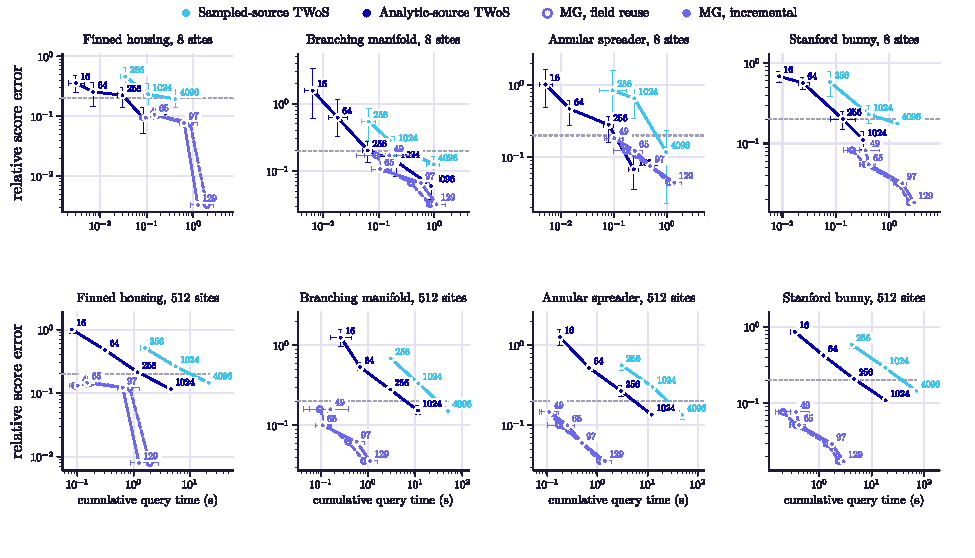
\includegraphics[width=\textwidth]{figures/matched-accuracy-original.pdf}
\caption{All measured budgets on the original domain, at 8 sites (top) and 512 sites (bottom). Bars are pointwise 95\% bootstrap intervals over five seeds; they exclude numerical-reference bias. Dashed horizontal lines mark the 20\% target before applying the independent reference gates. Numbers label path counts or longest-axis grid counts. Original and source-integrated TWoS and both grid reuse variants are retained.}\end{figure}
\begin{figure}[p]\centering
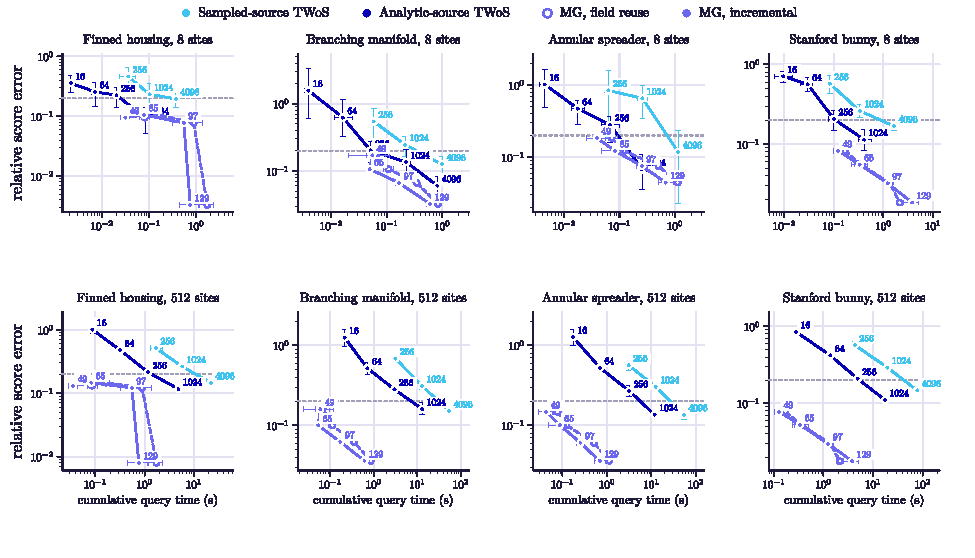
\includegraphics[width=\textwidth]{figures/matched-accuracy-edited.pdf}
\caption{All measured budgets on the edited domain, at 8 sites (top) and 512 sites (bottom). Bars are pointwise 95\% bootstrap intervals over five seeds; they exclude numerical-reference bias. Dashed horizontal lines mark the 20\% target before applying the independent reference gates. Numbers label path counts or longest-axis grid counts. Original and source-integrated TWoS and both grid reuse variants are retained.}\end{figure}
\begin{figure}[p]\centering
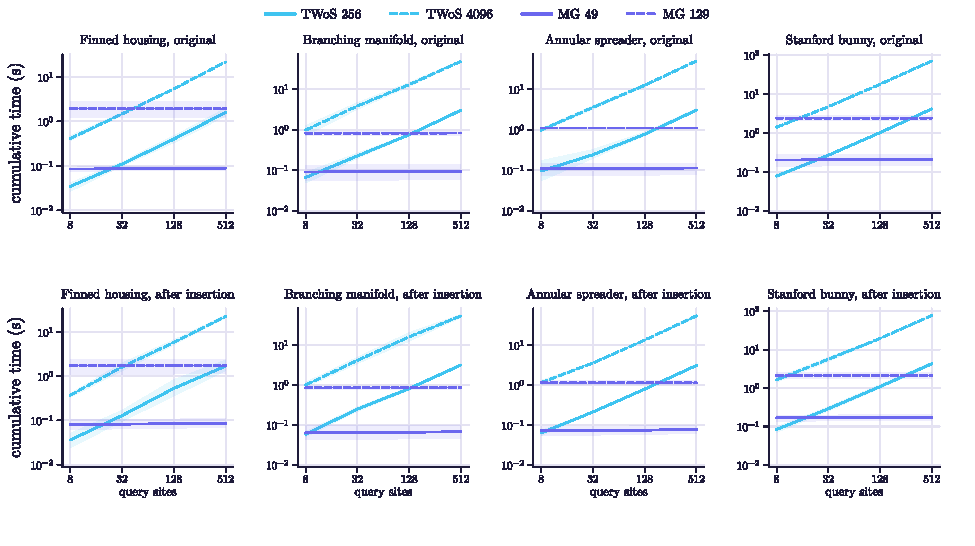
\includegraphics[width=\textwidth]{figures/matched-accuracy-scaling.pdf}
\caption{Measured query-count scaling at fixed budgets in the initially frozen sweep. Shaded bands show pointwise 95\% bootstrap intervals for mean time. Original-source TWoS scales with the number of sites, whereas solved-field multigrid amortizes its setup. These fixed-budget curves do not assert matched accuracy.}\end{figure}
\paragraph{Fresh-seed confirmation and its failures.}
The four apparent 20\%-target wins selected from calibration did not pass both fresh-seed rules. The three compliance cases exceeded the mean-error upper-endpoint threshold; the housing timing interval included no advantage. We then declared a separate, fixed 256-path follow-up for both eight-site compliance states, with 20 further fresh seeds and no subsequent budget search. All results are retained below. These pointwise bootstrap checks are not simultaneous confidence guarantees.
\begin{table}[t]\centering\small
\caption{Fresh-seed query confirmations. Times exclude common geometry loading. Error upper endpoints and speed intervals use 10,000 paired bootstrap resamples of 20 seeds. Passing requires error upper endpoint $\leq20\%$ and speed-ratio lower endpoint $>1$. Every row uses MG49.}
\setlength{\tabcolsep}{3.2pt}
\begin{tabular}{llrrrrrr}\toprule Workload / state & Stage & Sites & Paths & TWoS / MG (ms) & Error upper & MG/TWoS interval & Pass\\\midrule
Bunny compliance / edited & Selected & 8 & 64 & 23.3 / 78.4 & 21.8\% & [2.51, 4.57] & no\\
Bunny compliance / original & Selected & 8 & 64 & 28.7 / 341.3 & 21.3\% & [6.21, 19.36] & no\\
Bunny compliance / original & Selected & 32 & 64 & 74.0 / 136.8 & 20.8\% & [1.58, 2.13] & no\\
Housing / original & Selected & 8 & 1024 & 137.4 / 131.9 & 13.6\% & [0.58, 1.54] & no\\
Bunny compliance / edited & Fixed 256 & 8 & 256 & 83.1 / 72.8 & 10.3\% & [0.69, 1.11] & no\\
Bunny compliance / original & Fixed 256 & 8 & 256 & 89.9 / 113.9 & 10.2\% & [1.05, 1.50] & yes\\
\bottomrule\end{tabular}\end{table}


\paragraph{Random-stream indexing audit and correction.}
The retained legacy implementation XORs hashes of a seed, site index, and
walk index. When a driver seed equals a walk-index offset, this construction
can cancel or swap identifiers and reuse a stream across nominal repetitions.
For the present five seeds and four query batches, this affects twelve
indices at the 4,096-path budget; budgets through 1,024, the high-seed
reference batches, and the fresh holdout seeds do not have that structural
overlap. We correct the affected calibration draws, retain the superseded
outputs, and enumerate the resulting stream keys to check uniqueness.
This is a disclosed correctness amendment, not a selection based on outcomes.

Let $I$ be the fixed set of affected indices. We replay their original
paths and replacement paths with unused indices, obtaining $(U_i,P_i)$ and
$(U'_i,P'_i)$. The corrected sufficient statistics are
\[
 S'_U=N\bar U+\sum_{i\in I}(U'_i-U_i),\qquad
 S'_P=N\bar P+\sum_{i\in I}(P'_i-P_i),
\]
\[
 S'_{UP}=\sum_i U_iP_i+
       \sum_{i\in I}(U'_iP'_i-U_iP_i),\qquad
 \widehat S'=\frac{S'_US'_P-S'_{UP}}{N(N-1)}.
\]
To verify the reconstruction, split each original sum into indices inside
and outside $I$: subtraction removes exactly the old inside terms, and
addition supplies exactly their replacements. Thus these are precisely the
sums of the corrected $N$ pairs in exact arithmetic. Selection of $I$ depends
only on stream identities, so it does not condition on observed path values.
Under the ideal independent-stream model, unique keys give the intended
independent pairs and the usual off-diagonal-product proof applies. Distinct
PRNG keys alone are not a mathematical proof of PRNG independence.
We check floating-point reconstruction against complete clean runs on each
affected workload; all replay work is charged to corrected query costs.

\paragraph{Fresh-seed confirmation of apparent speed wins.}
Budgets selected from five calibration seeds are not independently validated
by those same seeds. Before measuring the extensions, we therefore fix a
confirmation protocol: every apparent 20\%-target speed win retains its
selected configurations and uses 20 fresh seeds, alternating method order.
The upper bootstrap mean-error endpoint must remain below 20\%, and the
lower paired runtime-ratio endpoint must exceed one, to call the result a
confirmed win. Failed confirmations remain reported. The same numerical
reference gates apply; these pointwise checks are neither simultaneous tests
nor continuum-error certificates. Offline tuning and reference construction
are excluded from query costs, so this comparison is not an online accuracy
controller.

\FloatBarrier
\section{A Source-Specific Rao--Blackwellized Variant}
\label{app:analytic-source}

This extension was added after the first housing comparison exposed poor
accuracy--cost performance of the original source-point estimator. It is
reported as a separate ablation, with the original measurements retained.
Analytic source integration and Rao--Blackwellization are standard variance
reduction ideas; we make no priority claim for either. The extension applies
to the prescribed radial polynomial loads in these benchmarks, not arbitrary
spatial source fields.

\paragraph{Step 1: construct a particular solution.}
For $A\geq0$ and $R>0$, consider one source $f(x)=A(1-\|x-c\|^2/R^2)_+^2$, set $d=\|x-c\|$ and
\[
 \Psi(d)=\begin{cases}
 AR^2\bigl(\frac16-\frac{d^2}{6R^2}
  +\frac{d^4}{10R^4}-\frac{d^6}{42R^6}\bigr),&d\leq R,\\
 \frac{8AR^3}{105d},&d>R.
 \end{cases}
\]
Inside the source, direct differentiation gives
\[
 \Psi'(d)=-A\left(\frac d3-\frac{2d^3}{5R^2}
                              +\frac{d^5}{7R^4}\right),
 \qquad -(d^2\Psi'(d))'=d^2f(d).
\]
Thus $-\Delta\Psi=f$ for $0<d<R$. At the origin the derivative vanishes
and the polynomial is smooth. Outside $R$, $1/d$ is harmonic. At $d=R$,
the two values equal $8AR^2/105$ and the two derivatives equal $-8AR/105$.
Consequently there is no distributional surface source at the join, and
$-\Delta\Psi=f$ globally. Linearity permits summing sources and using the
normalized sensor bump for the adjoint.

\paragraph{Step 2: integrate a walk ball exactly.}
Here $r$ denotes a walk-ball radius, not the inserted-cavity radius.
For the radius-$r$ ball centered at the current walk point $x$, the Poisson
representation gives the nonnegative source contribution
\[
 \begin{aligned}
 I(x,r)&=\int_{B_r(x)}G_{B_r(x)}(x,y)f(y)\,dy\\
       &=\Psi(\|x-c\|)-\frac1{4\pi}\int_{\mathbb S^2}\Psi(\|x+r\omega-c\|)\,d\omega.
 \end{aligned}
\]
This follows by subtracting the harmonic extension of $\Psi$ from $\Psi$
in the ball; their difference has zero boundary data and source $f$.
For $d>0$, parameterize the polar angle by $t=\cos\theta$. With
$s^2=d^2+r^2+2drt$, we have $dt=s\,ds/(dr)$ and therefore
\[
 \frac1{4\pi}\int_{\mathbb S^2}\Psi(\|x+r\omega-c\|)\,d\omega
 =\frac{1}{2dr}\int_{|d-r|}^{d+r}s\Psi(s)\,ds.
\]
An antiderivative for $s\leq R$ is
\[
 F(s)=A\left(\frac{R^2s^2}{12}-\frac{s^4}{24}
             +\frac{s^6}{60R^2}-\frac{s^8}{336R^4}\right).
\]
For $s>R$, continue it by $F(R)+8AR^3(s-R)/105$.
Hence the mean is $[F(d+r)-F(|d-r|)]/(2dr)$. For $d=0$ it is simply
$\Psi(r)$. If $d\geq r+R$, the source support misses the ball and $I=0$
exactly. If $d+R\leq r$, the sphere mean is $8AR^3/(105r)$.
These cases also avoid unnecessary cancellation in the implementation.

\paragraph{Step 3: retain the same score target.}
Let $\mathcal H_i$ contain the entire sphere-exit path of walk $i$, including
its termination, and let $(U_i,P_i)$ denote the original source-sampled
primal--adjoint pair. Source-point draws are independent of the sphere-exit
draws in the ideal sampling model. Exact ball integration yields
$\bar U_i=\mathbb E[U_i\mid\mathcal H_i]$ and
$\bar P_i=\mathbb E[P_i\mid\mathcal H_i]$. Different walks remain independent.
For $i\ne j$, conditional independence of their source draws gives
\[
 \mathbb E[U_iP_j\mid\mathcal H_1,\ldots,\mathcal H_N]
 =\bar U_i\bar P_j.
\]
Summing and dividing by $N(N-1)$ proves
\[
 \widehat S_{\rm RB}
 =\frac{\sum_{i\ne j}\bar U_i\bar P_j}{N(N-1)}
 =\mathbb E[\widehat S\mid\mathcal H_1,\ldots,\mathcal H_N].
\]
The tower property preserves expectation. For finite second moments, total
variance gives the precise guarantee
\[
 \operatorname{Var}(\widehat S)
 =\operatorname{Var}(\widehat S_{\rm RB})
  +\mathbb E\!\left[\operatorname{Var}(\widehat S\mid
                \mathcal H_1,\ldots,\mathcal H_N)\right]
 \geq\operatorname{Var}(\widehat S_{\rm RB}).
\]
This compares the same number of independent exit paths under exact source
integration; it does not guarantee lower wall time. It also preserves any
termination bias of the underlying walk model rather than removing it.
The earlier ideal-arithmetic variance upper bounds therefore remain valid
for this conditional estimator under the same moment assumptions.

\paragraph{Numerical implementation and scope.}
The implementation evaluates these expressions in long double and clamps
small negative roundoff to zero. Very small $d/R$ uses the centered limit.
These are numerical approximations to the ideal conditional expectation;
the variance inequality is not a finite-precision certificate. An independent
quadrature check accompanies the source. The measured extension uses the same
sites, seeds, accuracy gates, and reference fields as the original
study. Before measuring this variant, we additionally fix path budgets 16
and 64 alongside the original 256, 1,024, and 4,096, to test whether reduced
variance permits cheaper queries. It is compared to a stronger multigrid extension that retains outer
geometry masks and warm-starts the primal and adjoint after cavity insertion.
Both extensions are explicitly distinguished from the initially frozen sweep.

\paragraph{Checking the earlier distributed-heating regime.}
A separate Bunny experiment uses the earlier PDE type $f(x)=1+0.65x_y$
and compliance $J=\int_D fu$, so $p=u$. It uses the new fixed query sites
and cavity, not the exact historical site pool. Here the sphere-centered
Green kernel is radial. Odd moments vanish, hence
\[
 \int_{B_r(x)}G(x,y)f(y)\,dy
 =f(x)\int_{B_r(x)}G(x,y)\,dy=\frac{r^2}{6}f(x).
\]
The final equality follows by integrating
$\int_0^r(t-t^2/r)\,dt=r^2/6$. Thus affine-source integration is exact in
ideal arithmetic without using the radial-bump formula. TWoS estimates
$u^2$ with the same off-diagonal product. The 257-node reference required increasing the maximum V-cycle count from
120 to 800 while retaining the $10^{-7}$ residual tolerance; the same cap
is available to every grid budget in this compliance workload.
The multigrid baseline solves only
one field and reuses it for the adjoint; it also retains its mask and
warm-starts after insertion. This diagnostic was added after the three
engineering-geometry results, with the same five seeds, query counts,
reference gates, and targets. It uses the predeclared path budgets
$16,64,256,1024,4096$. Since cavity removal restricts the volumetric heat
source, it is a query comparison, not a fixed-total-heat design study.

\paragraph{Predeclared extension stopping rule.}
Before measuring either source-integrated extension, we fix the following
rule. Budgets 16, 64, and 256 are measured at every query count and both states.
Budgets 1,024 and 4,096 are measured only through the largest remaining
unresolved prefix in each state. A case closes when a previous budget meets
the strictest reference-resolved target among 10\%, 20\%, and 40\%, using
the unchanged upper bootstrap mean-error rule. A case with no resolved
reference target remains explicitly unresolved and does not trigger more
sampling. The saved records include every stopping decision. Thus the
extensions identify target-attaining budgets; they are not exhaustive
high-budget error--cost fronts. The original four-workload sweep is unchanged.

\FloatBarrier
\section{A Distinct Adjoint for Regional Thermal Protection}
\label{app:regional}

\subsection{Objective, adjoint, and the insertion score}
Fix a nonnegative weight $q$ supported in a protected region $S\Subset D$.
Require all admissible cavities to be disjoint from $S$ and set
$Q=\int_S q>0$. The physical source $f$ and the observation weight $q$
serve different roles. For the zero-Dirichlet Poisson state define
\begin{equation}
 -\Delta u_D=f\quad\hbox{in }D,\qquad
 J_q(D)=Q^{-1}\int_S q u_D.
 \label{eq:regionalobjective}
\end{equation}
Let $p_D$ solve $-\Delta p_D=q$ in $D$ with zero boundary data. This
unnormalized adjoint is convenient in the implementation; the actual
adjoint for $J_q$ is $p_D/Q$.

\begin{proposition}[Regional sensitivity and monotonicity]
Under the smoothness and separation assumptions of
\cref{thm:localtd}, the capacity-normalized derivative for a
zero-temperature cavity at $z\notin S$ is
\begin{equation}
 D_TJ_q(z)=-u_D(z)p_D(z)/Q.
 \label{eq:regionaltd}
\end{equation}
For finite nested domains obtained by removing cavities outside $S$,
$J_q$ is nonincreasing. This monotonicity does not establish a minimum
benefit, or certify a particular finite-radius prediction.
\end{proposition}
\begin{proof}
\textbf{Step 1: differentiate the objective in the state.}
For every $v\in H^1_0(D)$, the linear objective has derivative
$j'(u)[v]=Q^{-1}\int_D qv$. The adjoint weak equation is therefore
$\int_D\nabla v\cdot\nabla(p_D/Q)=Q^{-1}\int_D qv$.
The fixed support and cavity exclusion keep both $q$ and $Q$ unchanged
by every admissible insertion.

\textbf{Step 2: apply the cavity expansion with this adjoint.}
The state trace imposed on the inserted cavity is zero. Substitution
of $h_z=0$ and adjoint $p_D/Q$ into the established local coefficient
$-(u_D(z)-h_z)p(z)$ gives \cref{eq:regionaltd}. Multiplication by
the positive constant $Q$ does not change candidate rankings. This
specialization uses the classical coefficient; it is not a claim that
the underlying topological formula is new.

\textbf{Step 3: compare finite-domain states.}\par
Write $u_D^-=\max(-u_D,0)\in H^1_0(D)$. The weak equation gives
\[
 -\int_D|\nabla u_D^-|^2=\int_D f u_D^-\geq0.
\]
Both the gradient norm and the nonnegative right-hand side must vanish.
Poincar\'e's inequality and the zero trace imply $u_D^-=0$, hence
$u_D\geq0$. For $D'=D\setminus K$, the difference
$w=u_D-u_{D'}$ is weakly harmonic in $D'$, has zero outer trace, and
has nonnegative trace $u_D$ on the new cavity. Consequently
$w^-=\max(-w,0)$ has zero trace on all of $\partial D'$ and belongs
to $H^1_0(D')$. The harmonic weak equation gives
$-\int_{D'}|\nabla w^-|^2=0$. Poincar\'e's inequality again yields
$w^-=0$, or $w\geq0$. Hence
$J_q(D)-J_q(D')=Q^{-1}\int_S qw\geq0$. Applying this argument at
each insertion proves the finite nested-domain statement. It supplies
no positive quantitative lower bound beyond zero.
\end{proof}

\subsection{An exact counterexample to hottest-point placement}
\begin{proposition}[A hottest point need not maximize topological benefit]
On the unit ball in $\mathbb R^3$, take $f=1$ and
$q(x)=1+b x_1$ for $0<|b|<1$. For the unnormalized linear objective
$\int q u$, the hottest point is the origin, but the origin does not
locally maximize the insertion benefit $up$.
\end{proposition}
\begin{proof}
\textbf{Step 1: solve the state.} Writing $r=|x|$, the function
$u=(1-r^2)/6$ vanishes on the boundary and satisfies $-\Delta u=1$,
because $\Delta r^2=6$. Uniqueness of the weak Dirichlet solution
identifies this function as the state. It is strictly decreasing in
$r>0$, so its unique maximum is at the origin.

\textbf{Step 2: solve the adjoint.} The product rule gives
$\Delta(x_1r^2)=x_1\Delta r^2+2\nabla x_1\cdot\nabla r^2
=6x_1+4x_1=10x_1$. Consequently
\[
 p(x)=(1-r^2)\left(\frac16+\frac{b x_1}{10}\right)
\]
has zero trace and satisfies $-\Delta p=1+b x_1=q$.
Again uniqueness identifies the adjoint.

\textbf{Step 3: inspect the benefit at the hottest point.}
Direct multiplication gives
\[
 u(x)p(x)=(1-r^2)^2\left(\frac1{36}+\frac{b x_1}{60}\right),
 \qquad \partial_{x_1}(up)(0)=\frac b{60}\ne0.
\]
Moving a sufficiently small distance in the direction
$\operatorname{sign}(b)e_1$ therefore increases $up$, while it
strictly decreases $u$. Thus hottest-point ranking and topological
ranking are distinct even for the same self-adjoint Poisson operator.
This analytic example establishes a mechanism, not the size of the
benefit in the housing experiment.
\end{proof}

\subsection{Paired random walks and what cross-fitting removes}
At a candidate, one walk accumulates both the physical-source
contribution $U_i$ and the observation-source contribution $P_i$.
The spherical exits and Green-distributed source samples are shared
within a pair. Different complete pairs use separate random streams.
For $N\geq2$ the implementation evaluates
\begin{equation}
 \widehat s=\frac{(\sum_iU_i)(\sum_iP_i)-\sum_iU_iP_i}{N(N-1)}.
 \label{eq:regionalcross}
\end{equation}
\begin{proposition}[Expectation of the implemented product]
For independent identically distributed pairs with finite second
moments, write $\mu_U=\E U_i$, $\mu_P=\E P_i$. Then
$\E\widehat s=\mu_U\mu_P$, whereas
$\E[N^{-1}\sum_i U_iP_i]=\mu_U\mu_P+\Cov(U_i,P_i)$.
\end{proposition}
\begin{proof}
Expanding the product of sums and subtracting its diagonal leaves
$\sum_{i\ne j}U_iP_j$. There are exactly $N(N-1)$ ordered distinct
pairs. For each, independence gives
$\E[U_iP_j]=\E U_i\E P_j=\mu_U\mu_P$. Divide the sum by its
number of terms to obtain the first assertion. For the diagonal,
the defining identity for covariance is
$\E[U_iP_i]=\mu_U\mu_P+\Cov(U_i,P_i)$; averaging preserves it.
\end{proof}
Cross-fitting removes product-correlation bias. It does not remove
WoS termination error. In the ideal contained-ball model with
nonnegative sources, dropping the terminal values makes each
expectation a lower approximation of its state. The measured code
uses the existing approximate distance and finite-precision sampling
implementation and does not assert a rigorous bias magnitude.
The specialized compliance certificate cannot be substituted into
\cref{eq:regionalobjective}: its square-energy identity is specific
to compliance. These new designs use fresh ranking at a fixed count.
Radius-independent variance does not imply independence from the
observation region: a very small support of $q$ can itself make source
sampling difficult. The regional study fixes that support before varying
the estimator budget. Its source-sampling difficulty is distinct from
encountering a shrinking trial cavity.

\subsection{Sensor normalization and protected geometry}
The two observation regions are radius-$a=0.13$ balls centered at
$(\pm0.55,\pm0.18,-0.03)$, with the signs chosen together. Define
$q(x)=(1-|x-c|^2/a^2)_+^2$. Radial integration gives
\begin{align*}
 Q&=4\pi a^3\int_0^1 t^2(1-t^2)^2\,dt\\
  &=4\pi a^3\left(\frac13-\frac25+\frac17\right)
    =\frac{32\pi a^3}{105}.
\end{align*}
The sensor-ball volume is $4\pi a^3/3$, so its average weight is
$8/35$. Uniform sensor-ball probes therefore estimate $J_q$ as the
sample mean of $qu$ divided by $8/35$. Candidate centers obey
$|z-c|\geq a+r+0.02$; by the triangle inequality every point of the
radius-$r$ cavity is at least $0.02$ away from the protected ball.
Thus reducing the objective cannot be accomplished by deleting
the monitored region.

\subsection{Replicated designs and numerical reference checks}
\begin{table*}[t]
\centering\small
\caption{Regional design comparison. Reductions are means $\pm$ one standard error across five designs per sensor. Both wall-time columns include candidate preparation and the complete selection driver, averaged across sensor cases. Retained-mesh timings use one fresh server per design; dashes denote configurations not rerun with that backend. The extra multigrid resolutions are a supplementary sweep.}
\label{tab:regional}
\begin{tabular}{lrrrr}
\toprule
Method & Left reduction (\%) & Right reduction (\%) & Reload mesh (s) & Retain mesh (s) \\
\midrule
Random & $10.55\pm1.54$ & $10.23\pm3.14$ & 0.44 & 0.39 \\
WoS hottest & $36.47\pm2.22$ & $29.26\pm2.24$ & 3.63 & 1.19 \\
MG hottest & $38.15\pm1.03$ & $29.99\pm1.77$ & 6.07 & 4.88 \\
TWoS sparse & $50.87\pm1.46$ & $50.09\pm1.34$ & 3.66 & 1.22 \\
TWoS larger budget & $52.13\pm1.08$ & $51.84\pm0.52$ & 5.04 & 2.62 \\
MG TD (57) & $53.50\pm0.62$ & $52.53\pm0.84$ & 2.51 & 1.41 \\
MG TD (85) & $53.57\pm0.66$ & $52.45\pm0.82$ & 4.54 & -- \\
MG TD (113) & $53.30\pm0.57$ & $52.15\pm0.88$ & 8.38 & 7.13 \\
MG TD (169) & $53.57\pm0.66$ & $52.15\pm0.88$ & 40.00 & -- \\
\bottomrule
\end{tabular}
\end{table*}

The benchmark retains all final geometries, per-round candidate fields,
solver residuals, work counts, and timings. Five seeds change the shared
candidate set and stochastic streams. The two target regions are evaluated
separately on the same housing. Each final objective uses four independent
scrambled Sobol blocks of 128 uniform sensor-ball probes, with 256 fresh
WoS paths per probe. Evaluation streams are independent of selection and
shared between methods for paired comparisons. The table reports variation
across complete designs, not a confidence guarantee for arbitrary new inputs.
The separate reference solver evaluates the state at the same probes.
Across first-seed designs, the fourfold shell refinement changes measured reduction by at most $0.087$ percentage points. Refining the evaluation grid from $169\times109\times85$ to $225\times145\times113$ changes it by at most $0.255$ points. Across all primary and supplementary designs, WoS and the $169\times109\times85$ reference differ by at most $1.864$ points. These sensitivity checks do not bound the remaining discretization or sampling bias.


The primary design protocol and sampling budgets were fixed before the
first completed seed. That seed was inspected before the other four ran.
The supplementary grid resolutions were specified after that pilot and
before their measurements. All are retained. No improvement in the
cooling model or guarantee of accessible cooling follows from changing
the observation objective. The theoretical counterexample above and
the observed improvement over hottest-point placement show why temperature
alone need not characterize objective sensitivity. The adjoint supplies the
missing observation dependence in the topological formula; deterministic
topological derivatives exploit the same information.

\FloatBarrier
\section{Accessible Ball-Union Channels}
\label{app:accessible}

\subsection{A geometric access guarantee}
The following construction gives an explicit passage through an object.
It does not assert a cooling rate, pressure drop, or manufacturing tolerance.
Let $e$ be a unit vector, let $m\geq1$ be an integer, and put
$c_j=c_0+jhe$ for $j=0,\ldots,m$, where $0<h<2r$. Define the open channel
$C=\bigcup_{j=0}^m B_r(c_j)$ and
$\rho=\sqrt{r^2-h^2/4}>0$.

\begin{proposition}[A positive-width passage]
\label{prop:channelcore}
The channel $C$ is path connected and contains the straight tube
\[
 T=\{c_0+te+v:0\leq t\leq mh,\ v\cdot e=0,\ |v|<\rho\}.
\]
If $c_0$ and $c_m$ lie strictly on opposite sides of a slab containing
the closed object, the removed set $C$ supplies an open route between
the two exterior sides. In particular, the route has positive width;
it is not merely a point-contact chain.
\end{proposition}
\begin{proof}
\textbf{Step 1: choose a neighboring center.}
For each $t\in[0,mh]$, rounding $t/h$ to a nearest integer gives
$j\in\{0,\ldots,m\}$ with $|t-jh|\leq h/2$.
\textbf{Step 2: bound the distance.}
Orthogonality of $v$ and $e$ gives
\[
 |c_0+te+v-c_j|^2=(t-jh)^2+|v|^2
 <h^2/4+\rho^2=r^2.
\]
Thus every point of $T$ belongs to an open ball in $C$.
\textbf{Step 3: connect all channel points.}
Any point of a ball can be connected to its center by a segment in that
ball. The centerline belongs to $T$. Concatenating two radial segments
with a centerline segment connects any two points of $C$.
\textbf{Step 4: reach the exterior.}
The endpoint centers lie in the exterior by the slab assumption.
Following the centerline from one endpoint to the other therefore
gives a route in $C$, including its portions removed from the object.
The strict tube inequality establishes positive transverse clearance.
Intersecting the tube with the object need not give a single component
on an arbitrary shape, but every such portion communicates with the
same open route. This statement does not require the remaining material
to be connected.
\end{proof}

\begin{proposition}[Protection and channel separation]
\label{prop:channelprotection}
Let $a>0$ and $g\geq0$. For parallel channels of radius $r$, a transverse distance at least
$r+a+g$ from a protected ball's center to the channel axis gives
a gap of at least $g$ from that radius-$a$ ball. An axis separation
of at least $2r+g$ gives a gap of at least $g$ between channels.
\end{proposition}
\begin{proof}
\textbf{Step 1: enclose the channel.}
Every channel ball lies in the radius-$r$ cylinder around its axis,
so the union lies in that cylinder.
\textbf{Step 2: project protected points.}
Orthogonal projection onto the plane perpendicular to the axis cannot
increase distances. A point in the protected ball projects at distance
at most $a$ from its center's projection. A channel point projects at
distance at most $r$ from its axis. The reverse triangle inequality
therefore bounds their separation below by $(r+a+g)-a-r=g$.
\textbf{Step 3: apply the same argument to two channels.}
Their two projected radial distances are each at most $r$, giving
the lower bound $(2r+g)-2r=g$.
\end{proof}

\subsection{What the construction does not prove}
For the nonnegative-source, zero-Dirichlet model and a protected
observation region, domain removal still gives a nonincreasing
regional objective, provided the weak solutions and trace comparison
used in \cref{app:regional} apply. To see this, set $D'=D\setminus
\overline C$ and use exactly the difference $u_D-u_{D'}$ and its
negative-part test from that proof. The new trace is nonnegative and
the source agrees on $D'$, so the weighted integral difference is
nonnegative. No assertion that the channel is infinitesimal is needed
for this comparison.

However, $-u(z)p(z)$ is the coefficient for a separated small ball.
A channel consists of many overlapping balls and meets the exterior.
The single-ball expansion therefore does not justify summing their
coefficients or assigning a certified finite benefit to the whole
channel. The experiment uses the point score as a placement heuristic,
then independently evaluates the actual channel geometry. A stronger
channel-shape derivative or finite-insertion theorem remains separate
work. Nor does an open route justify ideal isothermal walls: flow,
convective heat transfer, external manifolds, and pumping power are
absent from the model.

\subsection{Reproducible experiment}
The new comparison uses two sensor positions, five paired candidate
seeds, and five methods. Each design adds six vertical channels of
radius $0.075$. Eighteen balls span $z=-0.45$ to $z=0.825$ with
spacing $0.075$, so \cref{prop:channelcore} gives the exact core radius
$0.075\sqrt{3}/2$. Endpoint coordinates are checked against the
actual boundary mesh's bounds. Channel axes avoid the sensor ball
and three radius-$0.07$ component balls, with a $0.02$ additional
gap; channels have a $0.025$ mutual gap. Components are centered at
the three prescribed source peaks. The Gaussian source tails remain
a volumetric field on surviving material; this is not a fixed-power
electronic-component model.

Each seed gives 512 common candidate axes. Scores are queried at
$z=-0.03$ in the current domain and all channel balls are added after
each selection. Sparse \method{} and WoS hottest-point placement use
12 scout walks and 192 fresh rescore walks on 24 candidates.
Multigrid evaluates the same pointwise topological coefficient at
$57\times37\times29$ or $113\times73\times57$ nodes; random feasible
placement supplies a geometric control. Both solver families retain
the outer mesh through each complete six-round design. Timings include
candidate preparation, geometry setup, adaptive selection, I/O,
and process startup and shutdown. Reference evaluations are separate.

Four independently scrambled 128-point sensor-probe blocks and 256
fresh walks per probe evaluate every final design. A separate
$113\times73\times57$ grid provides another numerical reference.
First-seed designs additionally receive a fourfold shell refinement
and a $169\times109\times85$ grid check. Neither reference is exact.
Four independent 32,768-point scrambled blocks estimate removed
material volume and the removed fraction of the prescribed source.
All methods share channel count, radius, axial extent, and constraints;
the nonuniform housing thickness means their removed volumes are not
exactly equal. We report those volumes rather than describing this as
an equal-volume comparison. Port positions are optimized, not fixed
connections to an external manifold.

\begin{table*}[t]
\centering\small
\caption{Accessible-channel comparison. Regional temperature reductions are means $\pm$ one standard error across five designs per sensor. Time and removed material are averaged across both sensors. All methods use six channels with the same radius and extent; volume varies with local housing thickness. Point scores are placement proxies, not derivatives of an entire channel.}
\label{tab:accessible}
\begin{tabular}{lrrrr}
\toprule
Method & Left reduction (\%) & Right reduction (\%) & Design time (s) & Removed material (\%) \\
\midrule
Random & $17.30\pm2.23$ & $10.74\pm2.48$ & 0.26 & 4.28 \\
WoS hottest & $43.78\pm1.89$ & $30.39\pm4.17$ & 1.00 & 4.24 \\
TWoS proxy & $55.74\pm1.35$ & $52.47\pm0.56$ & 1.02 & 4.22 \\
MG proxy (57) & $58.14\pm1.11$ & $56.95\pm0.28$ & 1.26 & 4.37 \\
MG proxy (113) & $58.14\pm1.11$ & $57.35\pm0.41$ & 6.55 & 4.36 \\
\bottomrule
\end{tabular}
\end{table*}

The saved-data audit verifies all 50 channel geometries and 240 nonrandom selections. All walks terminate before the step cap and all recorded multigrid solves meet the $10^{-8}$ residual tolerance. The largest first-seed shell-refinement change is $0.084$ percentage points; the grid-refinement change is $1.721$ points. Across all designs, the two primary numerical references differ by at most $3.133$ points. These are sensitivity checks, not bounds on the remaining numerical error.


\FloatBarrier
\section{Matched Geometry and Pipeline Study}
\label{app:submissionstudy}

\begin{figure}[t]
 \centering
 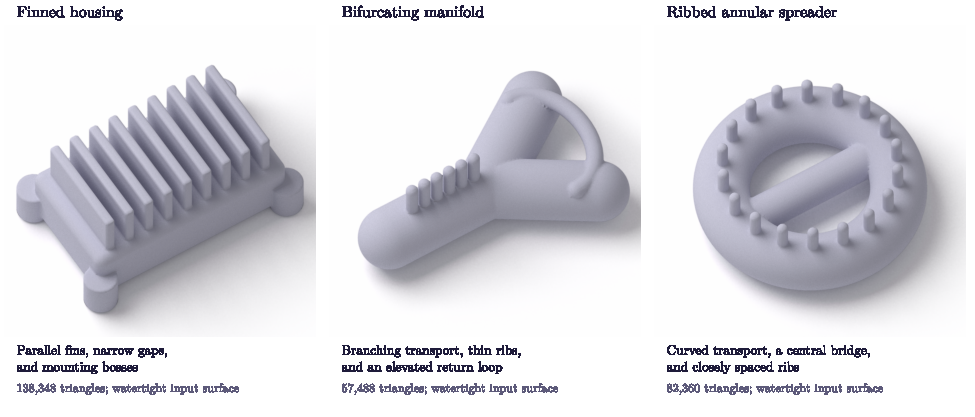
\includegraphics[width=\textwidth]{figures/submission-geometries.pdf}
 \caption{\textbf{Distinct application geometries.} Three watertight procedural
 test objects exercise different conduction paths and small geometric features.
 Every method uses the same surface, source configuration, and protected sensor
 within a case. Triangle count describes the input, not numerical difficulty.
 These are stylized conduction designs, not industrial cooling validations.}
 \label{fig:submissiongeometries}
\end{figure}

\subsection{A fixed-power, protected-region problem}
The additional study uses the same Poisson and ideal zero-Dirichlet cooling
model as the regional experiment, but replaces Gaussian source tails with
compact, fully protected heat components. This removes an ambiguity in the
fixed-count channel study: a lower objective can no longer result from deleting
a portion of a heat-generating source. All dimensions and temperatures are
nondimensional. No fluid or convective boundary model is implied.

For a center $c$, support radius $a>0$, and amplitude $A\geq0$, define
\[
 b_{c,a}(x)=\left(1-\frac{|x-c|^2}{a^2}\right)_+^2,
 \qquad f(x)=\sum_{j=1}^L A_j b_{c_j,a_j}(x).
\]
The sensor weight is $q=b_{s,b}/Q_b$, where $Q_b=32\pi b^3/105$.
The objective is $J(D)=\int_D q u_D\,dx$; the adjoint satisfies
$-\Delta p_D=q$ with homogeneous Dirichlet data. Component supports and the
sensor support are required to remain strictly inside the material.
The final protocol includes a low-power heat component of radius $0.085$
and amplitude $4$ at the protected sensor. This choice was fixed before the
measured campaign: an excluded remote-source-only pilot left the branching
sensor almost unheated and produced poorly resolved rare-event gradients.
The pilot is retained separately. Main heat sources remain stronger and
spatially distinct, so $f$ is not proportional to $q$.

\begin{proposition}[Exact normalization and preserved input power]
\label{prop:protectedpower}
Suppose $\overline{B_{a_j}(c_j)}\subset D$ for every $j$, and a removed set
$C$ is disjoint from these closed balls. Then
\[
 \int_{D\setminus\overline C} f\,dx
 =\int_D f\,dx
 =\sum_{j=1}^L\frac{32\pi A_j a_j^3}{105}.
\]
If $C$ also avoids $\overline{B_b(s)}$, then $\int_{D\setminus\overline C}q=1$.
For a point $X$ uniformly distributed in $B_b(s)$,
\[
 J(D)=\mathbb E\!\left[
 \frac{35}{8}\left(1-\frac{|X-s|^2}{b^2}\right)^2u_D(X)\right].
\]
\end{proposition}
\begin{proof}
\textbf{Step 1: restrict to the support.}
The positive-part definition makes $b_{c,a}$ zero outside $B_a(c)$.
Since this ball is contained in $D$ and untouched by $C$, its integral over
the original and the perforated domain is the same.
\textbf{Step 2: evaluate one radial integral.}
Translation and spherical coordinates give
\begin{align*}
 \int b_{c,a}(x)\,dx
 &=4\pi\int_0^a r^2(1-r^2/a^2)^2\,dr\\
 &=4\pi a^3\int_0^1(t^2-2t^4+t^6)\,dt\\
 &=4\pi a^3\left(\frac13-\frac25+\frac17\right)
 =\frac{32\pi a^3}{105}.
\end{align*}
\textbf{Step 3: sum the components.}
Linearity of the integral gives the displayed power identity. Disjointness
between heat components is unnecessary; only protection from removal is used.
\textbf{Step 4: normalize the sensor.}
Apply Step 2 with $(c,a)=(s,b)$ and divide by $Q_b$. Its support is unchanged,
so the integral of $q$ remains one.
\textbf{Step 5: express the objective as an expectation.}
The uniform-ball density is $1/V_b$ with $V_b=4\pi b^3/3$.
Consequently $\int q u=V_b\mathbb E[q(X)u(X)]$ and
$V_b/Q_b=35/8$, proving the formula. This identity concerns exact integrals;
finite quadrature and Monte Carlo estimates retain their numerical errors.
\end{proof}

\begin{proposition}[The local insertion coefficient for the new objective]
If a candidate $z$ lies outside all protected supports and satisfies the
regularity, separation, and cavity-expansion assumptions of the regional
result in \cref{app:regional}, then
\[
 \lim_{r\downarrow0}\frac{J(D\setminus\overline{B_r(z)})-J(D)}{4\pi r}
 =-u_D(z)p_D(z).
\]
\end{proposition}
\begin{proof}
\textbf{Step 1: identify the state and observation data.}
The compact bump and its first derivative vanish at its support boundary;
in particular the finite sums defining $f$ and $q$ are bounded and continuous.
The support-protection assumptions make both data independent of the inserted
cavity for all sufficiently small $r$.
\textbf{Step 2: specialize the regional objective.}
Its observation density is exactly the fixed, nonnegative $q$ above; the
adjoint is the solution of $-\Delta p=q$. The regional cavity expansion
therefore has coefficient $-u_D(z)p_D(z)$.
\textbf{Step 3: use the three-dimensional capacity convention.}
For the Laplacian convention used throughout the paper,
$\operatorname{cap}(B_r)=4\pi r$. Divide the expansion by this quantity and
let $r$ decrease to zero. The normalized remainder tends to zero under the
cited assumptions. This substitution provides no new remainder estimate,
and does not extend the separated-ball result to an overlapping channel.
\end{proof}

\subsection{Baselines and complete design costs}
Every pipeline starts from the same unperforated mesh, source configuration,
sensor, and paired candidate seed. We compare TWoS, deterministic multigrid
TD, deterministic hottest-point placement, and random placement of six
radius-$0.065$ spheres. The spheres remain disjoint and fully contained,
so every initialization and every subsequent translation removes exactly
$6(4\pi/3)(0.065)^3$ units of volume. Source and sensor clearance and a positive
inter-cavity gap are checked at every saved refinement state. Sphere centers
must remain at least $r+0.012$ from the outer boundary and at least
$r+a+0.018$ from each protected support center of radius $a$; pairs of
sphere centers must be separated by more than $2r+0.025$.

Each initialization is subsequently refined using our specialized implementation
of Differential WoS~\cite{miller2024differential}, Algorithm~2 and Eq.~(13).
For zero boundary data and inward offset $\ell$, a cavity-boundary hit contributes
$V_n\widehat u(x-\ell n)/\ell$ to the objective derivative; for a center
translation the parameter velocity has normal component $V_n=n\cdot v$.
The same radius, offset, gradient estimator, constraints, and backtracking
rule are used for all initializations. At each trial step, cavities are updated
in a cyclic order; each displacement is halved up to twelve times until feasible.
This avoids freezing all parameters when one cavity reaches a constraint. An
earlier global-rejection variant is retained as an excluded implementation
diagnostic; refinement and final evaluation were rerun for every method. TWoS and multigrid TD receive eight
refinement rounds; the hottest-point and random initializations additionally
receive rounds nine through sixteen. Independent evaluations at rounds
0, 4, 8, and, where applicable, 16 expose quality versus complete cost rather
than comparing only equal iteration counts. The two round allowances are not
identical wall-time budgets: distant initial cavities can produce few nonzero
boundary-gradient samples and consequently cheaper iterations. We therefore
report measured time explicitly and do not infer dominance at unmeasured budgets
or over all possible Differential WoS sampling schedules.

This is an attributed reimplementation of a paper component inside a common
benchmark, not the original authors' application optimizer. We checked the
terminal contribution and recursive boundary offset against the original authors' implementation. Differential WoS is not
in general restricted to topology-preserving changes. Here its fixed six-cavity
parameterization isolates initialization quality; this restriction is a choice
of comparison protocol, not a limitation claimed for that method.

TWoS uses 384 candidates, 48 scouting paths and 1,024 fresh rescore paths on
a 16-site shortlist per insertion. Multigrid solves for the primal and distinct
adjoint on a shared hierarchy with at most 65 nodes along the longest bounding-box
axis; other axis counts scale with the aspect ratio. It is our embedded Cartesian
finite-difference solver, not a finite-element implementation of another paper.
A separate complete-design baseline uses at most 49 nodes along the longest
axis with otherwise identical constraints and refinement. An additional
nearest-sensor control ranks candidates by Euclidean distance to the sensor
center and uses eight refinement rounds. It performs no PDE solve during
initialization, but shares every candidate and feasibility constraint. This
control tests whether simple proximity explains a benefit in the localized
observation task; it was added during the campaign as a baseline-strengthening
check, not selected through a parameter sweep. Independent resolution
checks use longest-axis counts 97 and 129. Convergence
to a $10^{-7}$ relative residual is checked separately from discretization error.

Complete design times include constructing the retained Embree geometry,
solver calls, request serialization, cavity selection, and all refinement or
radius-calibration decisions. Geometry generation, shared input preprocessing,
and independent evaluation are excluded. Backend high-water resident memory is
reported separately from driver memory. Instrumented outer-boundary distance
queries and parity rays are distinct counters; neither is inferred from the
number of walk steps. The measured campaign uses four OpenMP threads and single-threaded BLAS on
a Linux environment exposing an Intel Xeon Platinum 8573C, with an eight-CPU
quota and a 20 GiB memory limit. GCC 13.3 builds the C++17 backends with
\texttt{-O3}. Runs execute
serially without simultaneous rendering or other experiments. This is a
managed shared environment, not a dedicated timing node. The primary four
methods rotate order by seed; the two additional controls run subsequently,
so their timings should also be read in this execution context.

\paragraph{Guarded cavity offsets.}
A single ray-parity query can be ambiguous at a triangle edge. The following
geometric implication supplies a fallback specifically for contained spherical
cavities; it does not relax source protection or inter-cavity separation.

\begin{lemma}[An enclosing-ball test for a normal offset]
Let $D$ be open, $c\in D$, and $d=\operatorname{dist}(c,\partial D)>r+\ell$.
For any unit vector $e$, the point $c+(r+\ell)e$ belongs to $D$.
\end{lemma}
\begin{proof}
\textbf{Step 1: an open distance ball lies in the domain.}
If some $y$ with $|y-c|<d$ were outside $D$, the line segment from the
interior point $c$ to $y$ would first meet $\partial D$ at a point whose
distance from $c$ is at most $|y-c|<d$, a contradiction.
Thus $B_d(c)\subset D$.
\textbf{Step 2: apply the radius inequality.}
Since $|c+(r+\ell)e-c|=r+\ell<d$, this offset point belongs to $B_d(c)$,
and hence to $D$.
\end{proof}

The implementation retains its usual membership and analytic sphere-segment
checks. If the former rejects an offset, a positive enclosing-ball margin and
a checked interior cavity center provide an additional membership test. A
replay of the encountered case and an unchanged control are retained with
the benchmark. This is a numerical geometry guard under the stated mesh
assumptions, not a proof that floating-point distance and parity routines
are exact, and not the separate conservative application certificate.

\subsection{Finite-cavity estimator comparison}
Query timings use a retained outer-boundary acceleration structure, with
construction and an untimed warmup excluded for every estimator. Eight
protected, interior query sites are fixed per geometry before measuring
any estimator. A high-budget direct estimate uses sixteen independent batches
of 8,192 paths per site. Direct TWoS and common-random-number finite-cavity
differencing use sixteen repeats at 256 and 2,048 paths per site. For the latter,
the two state walks start at the same independently sampled sensor point and
use the same random stream in the original and perforated domain. Their
weighted difference is divided by $4\pi r$. Trial radii are
$0.08,0.04,0.02,0.01$. This is a specified local coupling, not a claim that
all possible finite-difference couplings have been optimized.

We additionally evaluate a stronger stopped-path baseline. It estimates the
finite cavity correction directly, rather than subtracting two noisy source
integrals. The following identity specifies precisely which quantity it estimates.

\begin{proposition}[A finite-cavity harmonic-correction estimator]
Let $D$ be bounded and let $D_r=D\setminus\overline{B_r(z)}$, with the cavity strictly contained and
disjoint from the sensor support. Let $u_D$ and $u_{D_r}$ solve the same Poisson equation $-\Delta u=f$ on their respective domains with zero Dirichlet data. Assume the domains are regular for the
Dirichlet problem and the state solutions are continuous up to their boundaries.
Let $Y$ be uniform in $B_b(s)$, let $X$ be a Brownian path started at $Y$, and
let $\tau_r$ be its first exit from $D_r$. Write
$W(Y)=(35/8)(1-|Y-s|^2/b^2)^2$ and
$H_r=\{X_{\tau_r}\in\partial B_r(z)\}$. Suppose $U_0(x)$ is a conditionally
unbiased, independent estimate of the original-domain temperature $u_D(x)$.
Then
\[
 Z_r=\frac{W(Y)\,\mathbf1_{H_r}\,U_0(X_{\tau_r})}{4\pi r}
 \quad\hbox{satisfies}\quad
 \mathbb E Z_r=\frac{J(D)-J(D_r)}{4\pi r}.
\]
The statement assumes the displayed expectation is integrable. Exact paths and
conditionally unbiased state estimates are mathematical assumptions here;
finite-termination implementations retain their numerical errors.
\end{proposition}
\begin{proof}
\textbf{Step 1: subtract the two PDEs.}
On $D_r$, both states have the same source, so $h=u_D-u_{D_r}$ satisfies
$-\Delta h=0$. On the old boundary, both states vanish and hence $h=0$.
On the cavity boundary, $u_{D_r}=0$ and hence $h=u_D$.
\textbf{Step 2: derive the harmonic exit representation.}
Fix $y\in D_r$. The difference $h$ is harmonic in $D_r$ and continuous on its
compact closure, hence bounded. Localize the Brownian motion to compact
interior subdomains and a finite time $t$. It\^o's formula for the localized
process has drift $(1/2)\Delta h=0$; its stochastic integral has zero mean
because the localized derivatives are bounded. Thus the expectation of the
stopped $h$ remains $h(y)$. Exhausting the domain gives the same equality
for $h(X_{t\wedge\tau_r})$ by dominated convergence. The exit time $\tau_r$
is finite almost surely: $D_r$ is contained in a ball, whose Brownian exit
time has finite expectation, and exiting $D_r$ occurs no later than exiting
that ball. Letting $t\to\infty$ and using boundedness and boundary continuity
therefore yields
\[
 h(y)=\mathbb E_y[h(X_{\tau_r})]
     =\mathbb E_y[\mathbf1_{H_r}u_D(X_{\tau_r})].
\]
The second equality uses exactly the two boundary values from Step 1;
it introduces no source-integral subtraction.
\textbf{Step 3: replace the boundary temperature by a fresh estimate.}
Condition on $Y$, the entire exit path, and its terminal point. Conditional
unbiasedness of the independent nested estimate gives
$\mathbb E[U_0(X_{\tau_r})\mid Y,X]=u_D(X_{\tau_r})$.
Applying the tower property therefore leaves the expression in Step 2 unchanged.
\textbf{Step 4: integrate the protected observation.}
The cavity does not remove any sensor weight. Proposition~\ref{prop:protectedpower}
and the tower property give
$\mathbb E[W(Y)h(Y)]=\int q(u_D-u_{D_r})=J(D)-J(D_r)$.
\textbf{Step 5: normalize.}
Divide this equality by $4\pi r>0$. The result is a finite-radius difference;
identifying its limit with $u_D(z)p_D(z)$ still requires the separate cavity
asymptotics. No finite-radius equality with that point product has been asserted.
\end{proof}

The implementation uses a perforated-domain boundary walk followed by one
independent original-domain source walk only on a new-cavity hit. It reports
the number of such hits, distance queries, time, and estimator variance. This
baseline tests the rare-event mechanism after removing unnecessary subtraction
noise. The common-random-number subtraction baseline is retained as a separate
implementation, rather than conflating the two couplings.

Variance about each estimator's own mean is kept separate from RMS error to
the high-budget infinitesimal reference. A finite-radius difference has a
different expectation from a topological derivative; its error includes this
remainder as well as sampling and termination error. The reference also has
sampling and termination error and is not labeled ground truth. Aggregate
errors weight high-influence sites more strongly; a reference with no sampled
contribution at a remote site does not establish a zero exact coefficient.
The data release reports reference standard error and the number of zero
reference estimates. A degenerate bootstrap interval from zero observed hits
likewise does not establish zero population variance. Multigrid
query estimates use longest-axis counts 49, 65, 97, and 129. Additional finite-hole
resolution checks explicitly expose grid differences that fail to resolve
the smallest cavities; a small linear-solver residual cannot resolve that issue.

\subsection{Matched finite channels}
Each channel is the union of balls at spacing $0.04$ along a vertical axis,
with centers from $z=-0.48$ to $0.80$. These endpoints lie beyond every
geometry's vertical bounds. For radius $r>0.02$, \cref{prop:channelcore} gives
a positive core radius $\sqrt{r^2-0.02^2}$. Parallel axes protect all compact
sources and the sensor by \cref{prop:channelprotection}. The shared candidate
pool is conservatively generated with maximum radius $0.11$, including the
source-clearance and axis-separation tests, even though calibrated radii are
usually smaller. This restriction is common to every method; the experiment
does not optimize over all feasible channel locations at the final radius.

After the $k$th axis is selected, a shared common radius is calibrated to
removed volume $0.0028k$ using a fixed scrambled Sobol sample of $2^{20}$
bounding-box points. Recalibration can change previous channels. Four independent
$2^{20}$-point scrambles audit the final volume; their dispersion is a numerical
integration diagnostic, not a certified enclosure. Six channels target total
volume $0.0168$. Neither equal radii nor equal channel counts are used as a
substitute for the volume measurement. The axis-point topological score remains
a heuristic for a finite channel, followed by independent objective evaluation.

\subsection{Evaluation, geometry, and visualization}
Five paired seeds are used on a finned housing, a bifurcating manifold with
thin ribs and an elevated return loop, and a ribbed annular spreader with a
central bridge. They are procedural application test objects, not standardized
industrial datasets. The latter two test branching and curved transport in
addition to the housing's narrow gaps and extended fins; surface triangle count
alone is not treated as evidence of numerical difficulty.

Each saved objective is evaluated in four independent scrambled-Sobol sensor
blocks of 128 points with 512 walks per point. The exact weight in
\cref{prop:protectedpower} is used. Paired-seed summaries retain the variation
between designs and separately report evaluation-block uncertainty. Additional
paired intervals jointly bootstrap the five design seeds and the four evaluation
blocks; block resampling is shared across methods and seeds to preserve the
common-random-number dependence. These are approximate, small-sample intervals,
not certified coverage guarantees. Reusing
the same evaluation blocks across methods supports paired differences; those
blocks never participate in candidate selection or line-search acceptance.
The housing-channel comparison exposed several percentage points of disagreement
between independent numerical references. We therefore added a uniform refinement
rule: a first-seed case is reevaluated at longest-axis counts 193 and 257 if any
method changes by more than 1 percentage point from grid 97 to 129 or differs
by more than 2 points between Monte Carlo and grid 129. Every method in a flagged
case is checked. This rule was introduced during reference auditing, rather than
claimed as a preregistered test; the added solves are excluded from design times.
Line search itself is heuristic and is not reported as certified.

\paragraph{Uncertainty bands and bars.}
Let $J_{m,k,b}$ be the independently evaluated objective for method $m$,
design seed $k\in\{1,\ldots,5\}$, and evaluation block
$b\in\{1,\ldots,4\}$, and let $J_{0,k,b}$ denote its unperforated reference.
The reported mean reduction is
\[
 \overline R_m=\frac15\sum_{k=1}^5
 100\left(1-\frac{\sum_b J_{m,k,b}}{\sum_b J_{0,k,b}}\right).
\]
For each of 4,000 bootstrap replicates, we resample five seed indices and four
block indices with replacement, then recompute this expression. The same indices
are used across methods and checkpoints, retaining the paired design and
common-random-number structure. Shaded trajectory bands are the pointwise
2.5th and 97.5th percentiles. Isolated channel results use vertical bars instead.
Horizontal bars resample measured complete-design times over the same seed
indices; they include both algorithmic and machine-timing variation. Faint
points show the individual design runs. Bands between checkpoints are visual
interpolation, not evaluations at every intervening time or simultaneous
confidence regions for an entire optimization path.

For an estimator setting, let $S_i\in\mathbb R^8$ be its vector of scores in
repeat $i$, and let $T_j\in\mathbb R^8$ be one of sixteen high-budget reference
batches. With $\overline T=16^{-1}\sum_jT_j$, the displayed relative variance
and RMS error are respectively
\[
 V=\frac{\sum_{a=1}^8\widehat{\operatorname{Var}}_i(S_{i,a})}
         {\|\overline T\|_2^2},\qquad
 E=\sqrt{\frac{\frac1n\sum_{i=1}^n\|S_i-\overline T\|_2^2}
                    {\|\overline T\|_2^2}}.
\]
We independently resample the sixteen repeat vectors and sixteen reference
batches 4,000 times. Sites remain together within each vector; treating sites as
independent experimental replicates would be inappropriate. Percentile bands
around $V$ measure uncertainty in the estimated variance, not the standard
deviation of an individual score. RMS-error bars additionally reflect sampling
uncertainty in the reference. A deterministic multigrid setting has one output:
its error bar reflects only reference sampling, and no Monte Carlo field variance is inferred. Timing intervals use five
additional repetitions per grid with rotated resolution order and a retained
outer mesh; each call rebuilds its multigrid hierarchy. All repeated fields
are checked against the original deterministic output. For the eight-site
query benchmark, a scheduling audit found that the original dynamic chunk of
four exposed only two work chunks to four threads. We repeat the direct-score
timing with chunk size one, verify every score and component field bitwise
against the retained original output, and use these repeats for query-time
plots. Original timings remain in the raw records. This correction changes
neither the numerical samples nor the recorded complete-design timings, which
retain their original scheduling. Numerical discretization, termination, offset,
and finite-radius bias are not enclosed by these bootstrap intervals. With only
five design seeds and sixteen estimator repeats, the intervals remain
approximate descriptive evidence, not established frequentist coverage or a
finite-insertion certificate. In particular, resampling cannot reveal rare
events absent from the recorded repeats; a zero observed score does not
establish zero temperature or influence. Site-level raw scores and cavity-hit
counts are retained for this reason. When all recorded correction vectors
are zero, we report the empirical output but suppress collapsed variance and
RMS-error intervals and mark variance unresolved. The earlier Bunny allocation bands in
\cref{fig:teaser,fig:bunnybudget} remain observed ranges over three designs;
they are not relabeled as confidence intervals.

Figures use the first predetermined seed, rather than selecting the visually
best design. Camera, section plane, display window, lighting, and map scale
are held fixed within each geometry. The local cooling map displays
$1-u_D(x)/u_{D_0}(x)$ on the visible material section using a longest-axis-193
multigrid field, clipped to $[0,1]$ for display. Material is gray where the
unperforated section temperature is below $10^{-4}$ of its maximum, avoiding
misleading relative changes in essentially cold material. Quantitative objective values
come from the separate evaluations above. A faint depth-tested shell shows
the physically present upper structure removed only for presentation.
The display cut, tessellated cavity surfaces, and lighting denoiser never enter
the PDE or its objective. Section colors are applied from the interpolated numerical field after
radiance denoising.

\begin{figure}[t]
 \centering
 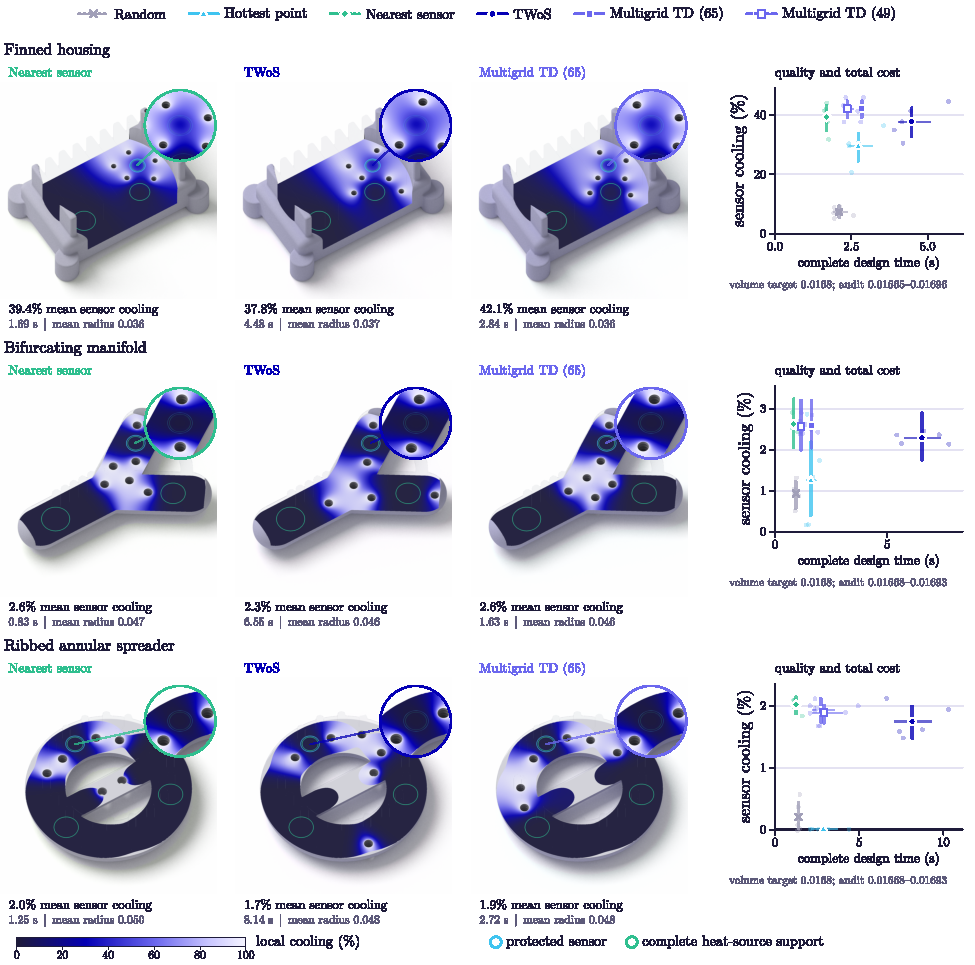
\includegraphics[width=\textwidth]{figures/submission-channels.pdf}
 \caption{\textbf{Accessible designs with controlled material and power budgets.}
 Six open ball-union channels are selected under identical source and sensor
 protection constraints. A common radius is calibrated to total removed volume
 $0.0168$; the displayed audit range spans the independent mean volume estimates
 over all methods and seeds in each geometry, not a certified interval.
 Heat input is exactly invariant under the protected-support model.
 Views use the first predeclared seed; quantitative summaries use five seeds.
 Vertical bars give pointwise 95\% bootstrap intervals for mean cooling,
 resampling seeds and independent evaluation blocks together across methods.
 Horizontal bars describe uncertainty in mean runtime across seeds; plot
 ranges adapt to each geometry while retaining the same physical units.
 The local cooling field shares a scale across designs. No coolant flow is
 solved, and the point score remains a heuristic for these extended removals.}
 \label{fig:submissionchannels}
\end{figure}



\FloatBarrier
\begin{table}[t]
\centering\small
\caption{\textbf{Complete cavity-design pipelines.} Means over five paired design seeds; SD is the sample standard deviation of their evaluated cooling reductions in percentage points, including evaluation noise. Cooling intervals are pointwise 95\% bootstrap intervals jointly resampling seeds and independent evaluation blocks. Backend RSS is process high-water memory, not total driver memory; a dash denotes no PDE backend call. Times include all design stages but exclude independent evaluation. Hot and random use sixteen refinement rounds; TWoS, multigrid, and nearest-sensor use eight.}
\label{tab:submissionpipeline}
\begin{tabular}{llrrrrr}
\toprule
Geometry & Method & Cooling (\%) & SD (pp) & 95\% interval & Time (s) & RSS (MiB) \\
\midrule
Finned housing & TWoS & 64.99 & 1.41 & [63.72, 66.20] & 11.77 & 24.2 \\
 & Multigrid TD (49) & 64.51 & 0.67 & [63.67, 65.26] & 7.99 & 24.2 \\
 & Multigrid TD (65) & 65.10 & 0.59 & [64.25, 65.94] & 8.66 & 24.4 \\
 & Nearest sensor & 63.56 & 2.60 & [61.31, 65.60] & 7.08 & 24.2 \\
 & Hottest point & 42.74 & 16.50 & [27.88, 51.06] & 13.14 & 24.3 \\
 & Random & 21.88 & 15.37 & [10.87, 34.92] & 10.69 & 24.1 \\
\midrule
Branching manifold & TWoS & 16.40 & 0.94 & [15.50, 17.38] & 51.24 & 14.1 \\
 & Multigrid TD (49) & 16.44 & 1.99 & [14.68, 17.91] & 43.21 & 14.0 \\
 & Multigrid TD (65) & 16.27 & 1.92 & [14.57, 17.69] & 43.76 & 14.1 \\
 & Nearest sensor & 17.33 & 0.80 & [16.43, 18.27] & 41.49 & 14.0 \\
 & Hottest point & 0.14 & 0.04 & [0.01, 0.35] & 13.43 & 14.0 \\
 & Random & 5.44 & 2.01 & [3.90, 7.37] & 46.65 & 13.9 \\
\midrule
Annular spreader & TWoS & 11.36 & 0.88 & [10.42, 12.26] & 35.78 & 17.4 \\
 & Multigrid TD (49) & 11.83 & 1.53 & [10.50, 13.17] & 30.30 & 17.5 \\
 & Multigrid TD (65) & 11.68 & 1.36 & [10.50, 12.88] & 29.67 & 17.6 \\
 & Nearest sensor & 12.19 & 2.12 & [10.26, 13.63] & 29.96 & 17.3 \\
 & Hottest point & 0.01 & 0.00 & [0.00, 0.02] & 10.73 & 17.4 \\
 & Random & 1.59 & 3.54 & [-0.00, 4.84] & 18.63 & 17.5 \\
\bottomrule
\end{tabular}
\end{table}

\begin{table}[t]
\centering\small
\caption{\textbf{Matched-volume accessible channels.} Means over five paired design seeds; SD is the sample standard deviation of their evaluated cooling reductions in percentage points, including evaluation noise. Cooling intervals are pointwise 95\% bootstrap intervals jointly resampling seeds and independent evaluation blocks. Backend RSS is process high-water memory, not total driver memory; a dash denotes no PDE backend call. Times include all design stages but exclude independent evaluation. Independent removed-volume audits are reported separately; every compact heat support is preserved.}
\label{tab:submissionchannels}
\begin{tabular}{llrrrrr}
\toprule
Geometry & Method & Cooling (\%) & SD (pp) & 95\% interval & Time (s) & RSS (MiB) \\
\midrule
Finned housing & TWoS & 37.79 & 5.48 & [32.92, 42.35] & 4.48 & 24.1 \\
 & Multigrid TD (49) & 42.11 & 3.00 & [39.13, 44.68] & 2.37 & 24.2 \\
 & Multigrid TD (65) & 42.11 & 3.00 & [39.13, 44.68] & 2.84 & 24.1 \\
 & Nearest sensor & 39.37 & 4.77 & [34.93, 43.05] & 1.69 & --- \\
 & Hottest point & 29.48 & 5.64 & [24.56, 33.80] & 2.73 & 24.3 \\
 & Random & 7.31 & 1.74 & [5.57, 9.29] & 2.10 & --- \\
\midrule
Branching manifold & TWoS & 2.29 & 0.14 & [1.74, 2.89] & 6.55 & 14.1 \\
 & Multigrid TD (49) & 2.57 & 0.23 & [2.00, 3.20] & 1.16 & 13.9 \\
 & Multigrid TD (65) & 2.59 & 0.16 & [2.05, 3.19] & 1.63 & 14.0 \\
 & Nearest sensor & 2.62 & 0.18 & [2.05, 3.23] & 0.83 & --- \\
 & Hottest point & 1.25 & 1.14 & [0.40, 2.18] & 1.60 & 14.0 \\
 & Random & 0.93 & 0.29 & [0.57, 1.21] & 0.93 & --- \\
\midrule
Annular spreader & TWoS & 1.75 & 0.27 & [1.48, 1.99] & 8.14 & 17.6 \\
 & Multigrid TD (49) & 1.89 & 0.13 & [1.73, 2.01] & 2.91 & 17.4 \\
 & Multigrid TD (65) & 1.93 & 0.16 & [1.74, 2.12] & 2.72 & 17.3 \\
 & Nearest sensor & 2.02 & 0.11 & [1.88, 2.15] & 1.25 & --- \\
 & Hottest point & 0.00 & 0.00 & [-0.00, 0.01] & 2.87 & 17.3 \\
 & Random & 0.20 & 0.25 & [0.02, 0.44] & 1.40 & --- \\
\bottomrule
\end{tabular}
\end{table}

\begin{table}[t]
\centering\small
\caption{\textbf{Independent resolution check.} First predeclared seed, before sphere refinement. Ranges span all six methods on each geometry. The grid columns give longest-axis node counts. Differences are percentage points of objective reduction. These comparisons test reference sensitivity; neither numerical method is exact ground truth.}
\label{tab:submissionreference}
\begin{tabular}{llrr}
\toprule
Study & Geometry & Grid 129 minus 97 (pp) & MC minus grid 129 (pp) \\
\midrule
Pipeline & Finned housing & [-1.30, -0.07] & [1.56, 3.18] \\
Pipeline & Branching manifold & [-0.01, 0.49] & [-0.15, 1.82] \\
Pipeline & Annular spreader & [-0.00, 0.37] & [0.00, 1.26] \\
Channels & Finned housing & [-2.60, -0.05] & [2.03, 4.79] \\
Channels & Branching manifold & [-0.01, 0.21] & [-0.01, 0.34] \\
Channels & Annular spreader & [-0.11, 0.03] & [-0.08, 0.04] \\
\bottomrule
\end{tabular}
\end{table}
\begin{table}[t]
\centering\small
\caption{\textbf{Finer reference checks for flagged cases.} A case is refined when any method changes by more than 1 pp from grid 97 to 129, or differs by more than 2 pp between MC and grid 129. Every method in that case is checked. Ranges span all six methods; sphere states are before refinement.}
\label{tab:submissionfinereference}
\begin{tabular}{llrr}
\toprule
Study & Geometry & Grid 257 minus 193 (pp) & MC minus grid 257 (pp) \\
\midrule
Pipeline & Finned housing & [-0.07, 0.44] & [0.47, 2.38] \\
Channels & Finned housing & [-0.17, 0.03] & [0.71, 2.12] \\
\bottomrule
\end{tabular}
\end{table}

\FloatBarrier
\section{Additional Figures for Earlier Thermal Studies}
\label{app:earlierthermalfigures}
These figures retain the earlier studies' original protocols and data. Their
budgets differ from the matched-volume, fixed-power, complete-pipeline
comparison in \cref{sec:submissionstudy}; their reported speed ratios and
uncertainty summaries should not be transferred between experiments.

\begin{figure}[t]
 \centering
 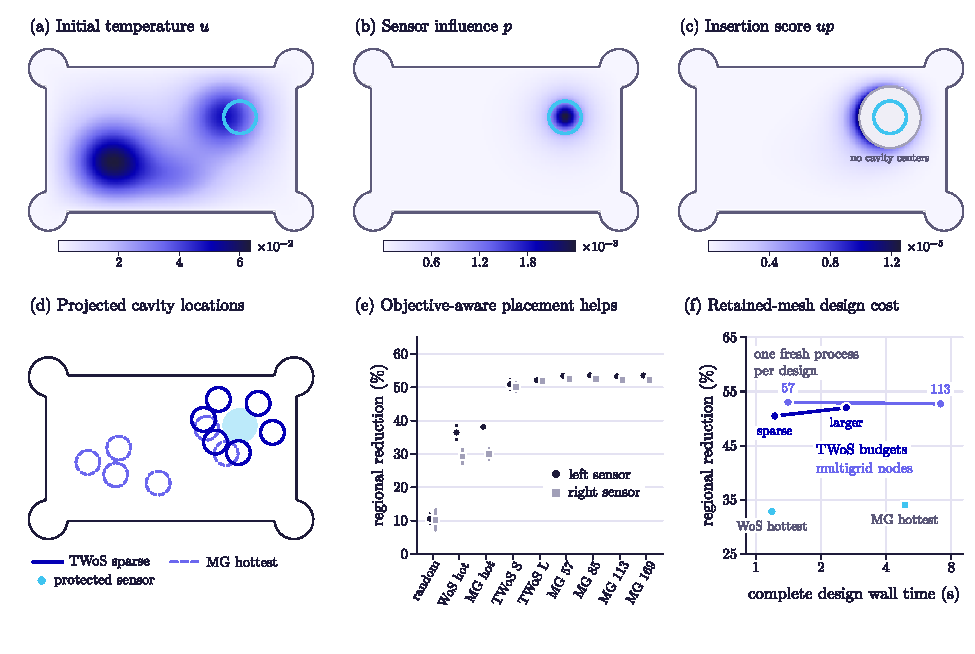
\includegraphics[width=\textwidth]{figures/distinct-adjoint-benchmark.pdf}
 \caption{Regional thermal protection with a distinct adjoint.
 (a--c) Initial temperature, sensor influence, and insertion scores on
 the same horizontal cut; each field has its own color scale.
 Cyan outlines the protected sensor; the light disk in (c) excludes
 cavity centers by the sensor radius, cavity radius, and safety gap.
 (d) Projected cavity spheres
 selected by sparse \method{} and deterministic hottest-point placement
 for the first right-sensor seed. (e) Regional temperature reductions,
 with one standard error across five complete designs. S and L denote
 the two \method{} sampling budgets. (f) Mean design quality and complete
 wall time across both sensor cases using the retained-mesh backend,
 showing both sampling budgets and the coarse/primary multigrid settings.
 The complete resolution sweep and both backend timings are in
 \cref{tab:regional}. Numerical references remain approximate;
 no finite-benefit certification is enabled in this experiment.}
 \label{fig:regional}
\end{figure}

\begin{figure}[t]
 \centering
 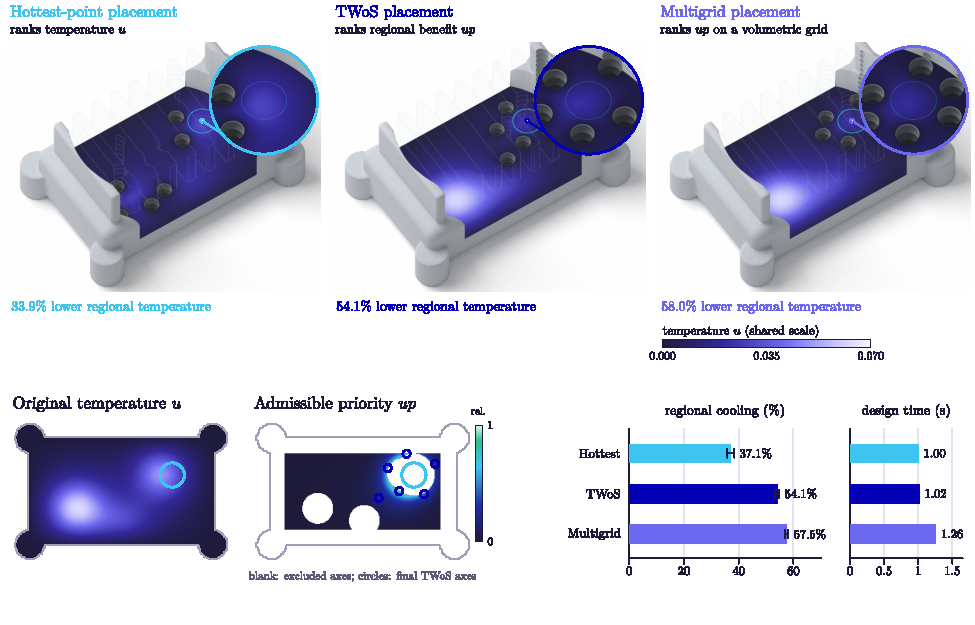
\includegraphics[width=\textwidth]{figures/accessible-channels.pdf}
 \caption{Accessible cooling with objective-aware placement.
 Top: actual saved first-seed right-sensor designs for hottest-point,
 TWoS, and coarse multigrid placement, with identical cameras, display cuts,
 lighting, and an absolute temperature scale. Magnified views show the
 protected sensor (cyan); cavity walls retain geometric shading. Faint,
 depth-tested shells indicate bars removed only for the display cut.
 The displayed cut does not enter the physical PDE. Section temperatures
 use a separate $169\times109\times85$ multigrid reference and bilinear
 display interpolation. Per-design labels use independent WoS evaluations.
 Bottom left: the original temperature and relative admissible $up$
 priority; circles mark the final TWoS axes, selected sequentially as
 fields change. Bottom right: mean cooling and complete design cost over
 both sensor positions and five seeds; error bars are one standard error
 across the five paired-seed averages. The full 50-design study, including
 random and finer-grid baselines, is in \cref{tab:accessible}.
 All methods share channel count, radius, and extent; removed volume varies.
 The point score remains a whole-channel placement heuristic, with no
 channel derivative or finite-benefit certificate asserted.}
 \label{fig:accessible}
\end{figure}

\begin{figure}[t]
 \centering
 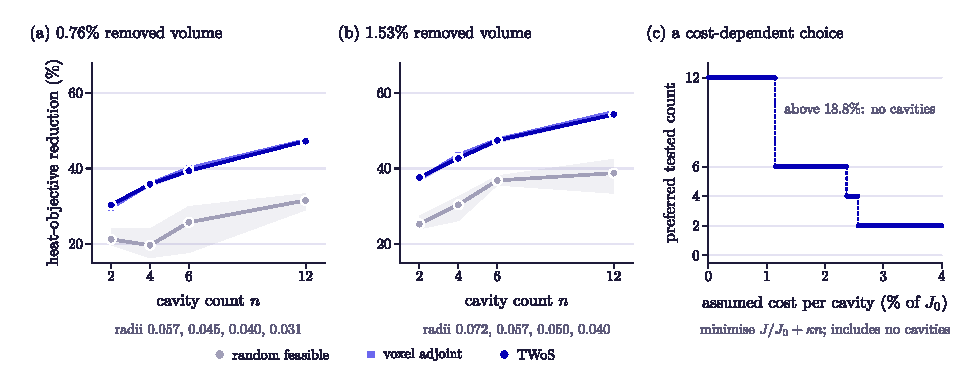
\includegraphics[width=\textwidth]{figures/bunny-budget.pdf}
 \caption{\textbf{Cavity allocation and a cost-dependent count.}
 (a--b) Cooling at two fixed removed volumes; radii are listed in count order.
 Lines are means over three complete design seeds, and shaded ranges are their
 minima and maxima, not confidence intervals. Each design is evaluated using
 four independent randomized spatial blocks with fresh WoS paths; blocks are
 shared across designs. (c) The preferred tested full-budget TWoS count after
 adding an assumed per-cavity cost to normalized compliance; the unperforated
 option is included. This is a finite-design sensitivity plot, not an estimated
 physical cost or a global optimum. All cavities have ideal cooled walls;
 at fixed volume, their total surface area increases with count.}
 \label{fig:bunnybudget}
\end{figure}

\begin{figure}[t]
 \centering
 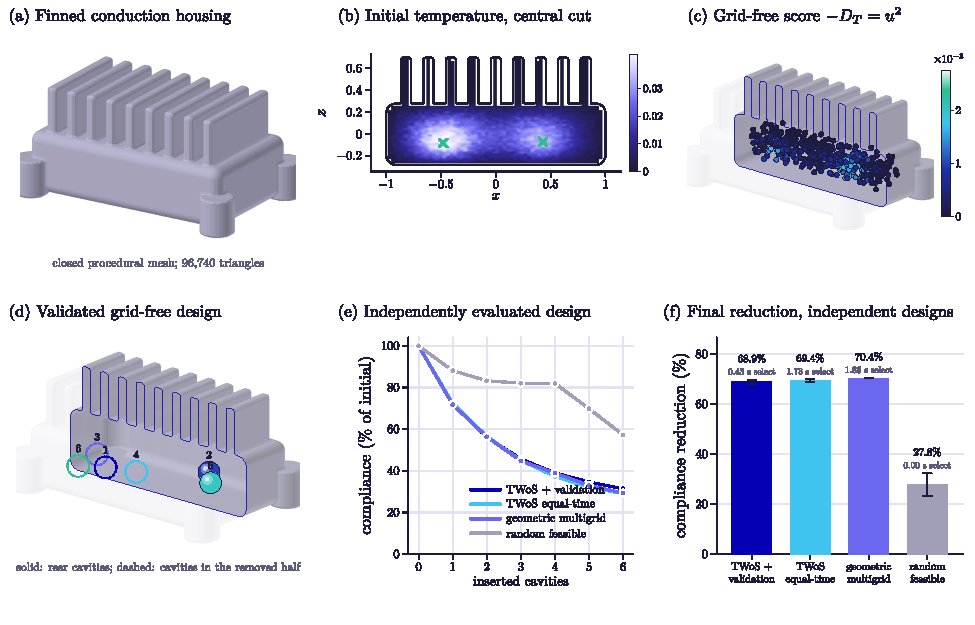
\includegraphics[width=\textwidth]{figures/engineering-housing-benchmark.pdf}
 \caption{Measured topology design on a stylized finned conduction housing.
 (a) The closed 96,740-triangle input. (b) Initial temperature on the central
 cut, with mint crosses at the two chip-source centers. (c) Direct grid-free
 topological scores inside a shaded cutaway. (d) Six cavities selected by
 scout--rank--fresh-validate; solid spheres lie in the retained half and
 dashed outlines lie in the removed half. (e) Compliance for one canonical run under
 independent reevaluation after every insertion. (f) Mean final reduction
 across five complete stochastic designs, with standard error and mean total
 selection time; multigrid uses one deterministic design and ten fresh
 objective streams. In this earlier figure, ``validation'' denotes fresh
 shortlist ranking samples; it is not the finite-benefit certificate.}
 \label{fig:housing}
\end{figure}

\FloatBarrier
\section{Detailed Experimental Protocols and Results}
\label{app:experiments}

\subsection{Controlled statistical diagnostics}

\paragraph{Annulus rare-event benchmark.}
Let the outer disk have radius one, start Brownian motion at $r_0=0.35$, and insert a concentric cavity of radius $\eps<r_0$.  Both the relative capacity
$\rho(\eps)=2\pi/\log(1/\eps)$ and the cavity-hit probability
$q_\eps=\log(1/r_0)/\log(1/\eps)$ are exact.  This diagnostic uses a pointwise harmonic response, outside the $L^2$-smooth objective assumptions of \cref{thm:localtd}. Taking the coupled path difference to be minus the hit indicator gives the exact normalized target
$D_T=-\log(1/r_0)/(2\pi)=-0.16708$.  We compare direct cross-fitted harmonic-measure queries, the common-random-number hit estimator, and two independent objective samples.  We use $N=256$, 3,000 independent replications, twelve radii from $10^{-1}$ through $10^{-24}$, percentile-bootstrap variance intervals, and fit slopes on the smaller-capacity half of the sweep.

\paragraph{Correlation benchmark.}
We draw 30,000 batches of $N=32$ Gaussian oracle pairs with means $(0.8,0.65)$, standard deviations $(0.5,0.6)$, and within-pair correlation swept from $-0.9$ to $0.9$.  The exact target is $D_T=-0.52$.  Same-seed multiplication, the product of sample means, cross-fitting, and fully independent primal/adjoint batches are evaluated on identical parameter settings.  Dotted curves in \cref{fig:controlled}(b) are the exact covariance-bias formulas.

\paragraph{Adaptive-selection benchmark.}
We search $K$ independent null sites whose estimates are Gaussian with known standard error $1/\sqrt{64}$.  A one-sided $5\%$ upper bound drives insertion.  Across 40,000 replications, we compare reusing the selected scouting estimate, a Bonferroni simultaneous bound on the scout, and a fresh pointwise validation estimate.  Wilson intervals quantify Monte Carlo uncertainty.



The fitted slopes in \cref{fig:controlled}(a) are $0.00$, $-1.10$, and $-1.89$ for direct, coupled, and independent estimation, respectively.  At the smallest tested capacity, direct \method{} has variance $7.06\times10^{-4}$, $8.26\times$ below coupled finite-cavity differencing and $80.4\times$ below independent differencing.  This crossover is the intended claim: finite differencing can be competitive for large holes, but becomes progressively worse in the topological limit.

At correlation $0.9$, the same-seed product has bias $-0.2708$, the product of means has bias $-0.00919$, cross-fitting has bias $-7.50\times10^{-4}$, and independent batches have bias $7.50\times10^{-4}$.  The latter two deviations are within their Monte Carlo standard errors.  Cross-fitting does not dominate independent batches in variance; it preserves unbiasedness while permitting shared trajectories or caches.  After selecting among $K=256$ null sites, naive reuse falsely inserts in $100.0\%$ of trials.  Bonferroni and fresh validation yield $4.985\%$ and $5.003\%$, with 95\% Wilson intervals $[4.776,5.203]\%$ and $[4.793,5.221]\%$, respectively.

\subsection{Spatial manufactured WoS field}

We next test the complete spatial estimator rather than only abstract oracle pairs.  In the unit disk, choose the harmonic polynomials
\begin{align}
 u(x,y)&=0.28+0.58x-0.30y+0.22(x^2-y^2),\\
 p(x,y)&=0.46-0.38x+0.34y+0.40xy.
\end{align}
Their boundary traces define two independent harmonic Dirichlet problems.
The analytic target is the product $-up$. Because the second field has
nonzero boundary data, it is not the homogeneous-boundary adjoint in
\cref{eq:adjointweak}; this is a product-estimator diagnostic, not a
manufactured design objective. The Poisson-compliance disk experiment in
\cref{sec:critical} tests an actual topological derivative.  A vectorized WoS implementation queries 6,359 sites in the compact disk $\|z\|\le0.88$, using 96 paired walks per site and a $10^{-7}$ termination shell.  Walks take 22.5 spheres on average.

\begin{figure}[t]
 \centering
 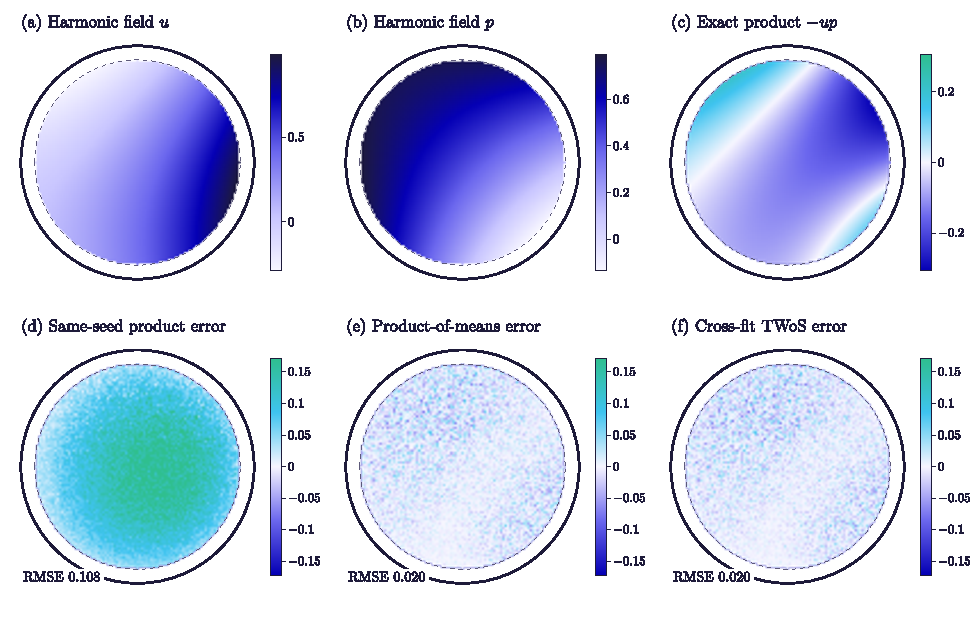
\includegraphics[width=0.96\textwidth]{figures/manufactured-field.pdf}
 \caption{Manufactured spatial validation with actual WoS paths. The two harmonic fields (a--b) and exact product $-up$ (c) supply analytic reference values. Multiplying same-seed primal and adjoint samples creates a coherent covariance-error field (d), with RMSE $0.108$ and mean bias $0.0987$. The product of sample means (e) suppresses the error to RMSE $0.0195$ but retains its finite-$N$ covariance bias. Cross-fitted \method{} (f) has RMSE $0.0196$ and mean bias $-1.20\times10^{-4}$, matching the sampling error while removing the bias exactly in expectation.}
 \label{fig:manufactured}
\end{figure}

\subsection{Three-dimensional internal-cooling reference}

We next exercise scout--rescore--insert placement in three dimensions.
The solid is the box
$[-1.2,1.2]\times[-0.8,0.8]\times[-0.45,0.45]$ with zero-temperature
Dirichlet data on its exterior and on every inserted cooling cavity.  We solve
$-\Delta u=f$ for the positive affine source
$f(x,y,z)=1+0.45x/1.2-0.25y/0.8$ and minimize the thermal compliance
$J=\int_\Omega fu\,dx$.  Since the adjoint equals the state, the normalized
spherical-cavity derivative is $D_T=-u^2$.  Affinity of $f$ makes the source
contribution on every three-dimensional WoS ball exact:
$f(x)R^2/6$.  Both the box and the union of cavities are queried analytically;
the TWoS method therefore constructs no volume grid.

We choose seven cavities of radius $0.115$ among 2,048 scrambled-Sobol
candidate centers, subject to identical exterior and pairwise clearances for
all methods.  Our method uses 16 walks per scouting site, freshly rescores a
24-site shortlist with 192 walks per site, and maximizes the resulting 95\%
lower confidence bound.  We compare against reusing the noisy scout, a
$49\times33\times19$ voxel adjoint/TD solve, and random feasible insertion.
Every design is evaluated on a fixed independent Sobol probe set with fresh
WoS paths; the optimization samples are never reused for the reported
objective.

\begin{figure}[t]
 \centering
 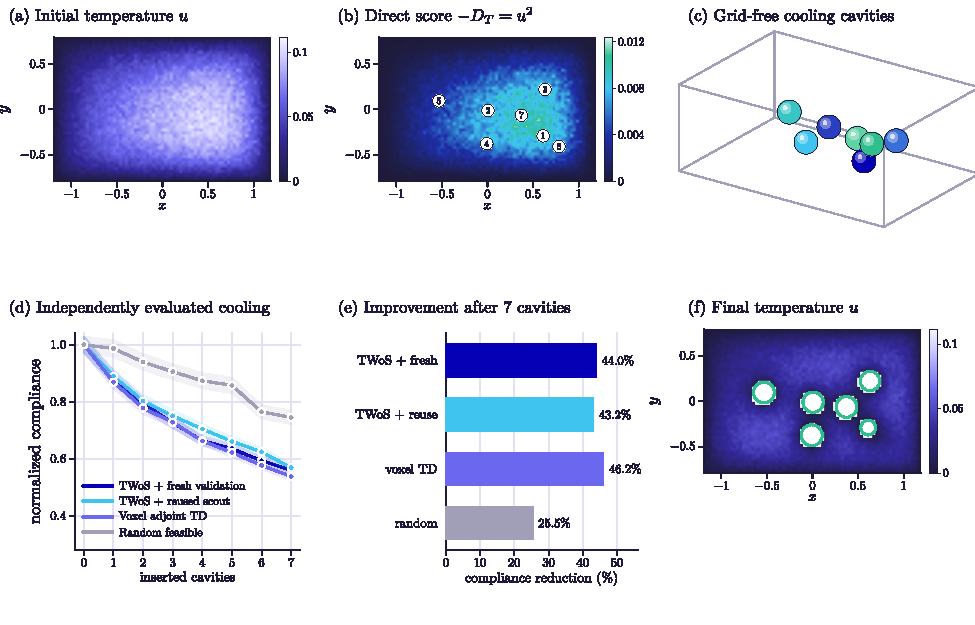
\includegraphics[width=\textwidth]{figures/internal-cooling-benchmark.pdf}
 \caption{Correctness-first 3D internal-cooling benchmark. (a) The initial
 temperature field on the central plane. (b) The direct cross-fitted
 topological score, with selected cavity centers projected onto the plane.
 (c) The resulting grid-free 3D cavity configuration. (d) Independently
 evaluated compliance throughout optimization. (e) Final improvement under
 the same seven-cavity budget. (f) The final central-plane temperature. This
 analytic-geometry pilot validates the complete application loop; it is not
 the final equal-time mesh benchmark.}
 \label{fig:coolingreference}
\end{figure}

The initial TWoS and voxel TD fields have Pearson correlation $0.977$ and
relative RMSE $0.104$.  After seven insertions, validated TWoS reduces
compliance by $43.99\%$, compared with $43.15\%$ for scout reuse, $46.17\%$
for the voxel reference, and $25.47\%$ for random insertion.  Thus the direct
grid-free estimator realizes $95.3\%$ of the voxel baseline's measured
reduction and $1.73\times$ the reduction of random placement.  The small gap
between fresh validation and scout reuse is not statistically resolved in this
single design run; the post-selection coverage experiment in
\cref{fig:controlled}(c), rather than this trajectory, supports the statistical selection mechanism in an idealized known-noise setting. It does not establish finite-cavity coverage for this 3D example.  We likewise withhold a timing claim: the current TWoS
reference is vectorized Python, whereas the sparse voxel solve runs in compiled
code.  The separate compiled Bunny and housing studies measure performance with matched C++ implementations.

\subsection{Stanford Bunny curved-mesh stress test}

The analytic box isolates the optimization mechanism but does not exercise a
production-style curved boundary.  We therefore repeat the complete loop
inside the canonical Stanford Bunny~\cite{stanford1994bunny}.  This experiment
is a geometry stress test, not an engineering claim about cooling a rabbit.
The original zippered reconstruction stores 35,947 vertices and 69,451
triangles and contains five holes in its bottom.  Our deterministic
preprocessing removes 1,113 unreferenced vertices, consistently orients the
faces, seals boundary loops of lengths 22, 42, 39, 40, and 80, and verifies a
closed edge- and vertex-manifold surface with Euler characteristic two.  The
result has 34,839 vertices and 69,674 triangles.

After normalizing the Bunny height to one, we solve the same Poisson-compliance
problem with affine source $f(x,y,z)=1+0.65(y+0.5)$.  We insert six cavities of
radius $0.05$ among 1,024 interior candidate centers.  Exact closest-triangle
distances come from a libigl AABB tree; candidate containment uses fast winding
numbers.  TWoS uses 12 scouting walks and freshly rescores a 20-site shortlist
with 128 walks per site.  The voxel reference uses a
$54\times64\times48$ Cartesian grid clipped by the Bunny.

\begin{figure}[t]
 \centering
 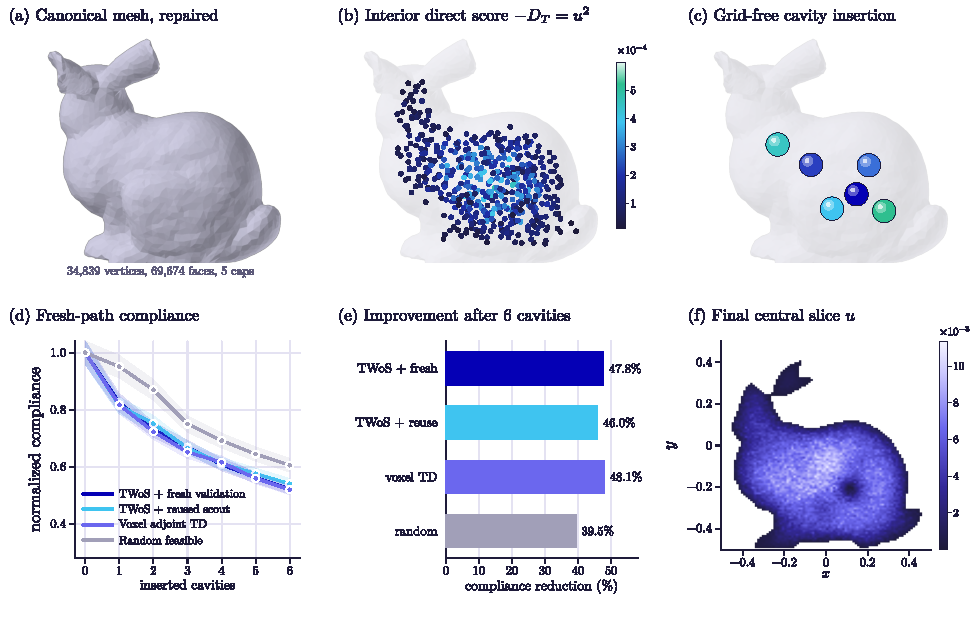
\includegraphics[width=\textwidth]{figures/stanford-bunny-benchmark.pdf}
 \caption{Curved-mesh geometry stress test on the Stanford Bunny. (a) The
 repaired closed input mesh. (b) Interior cross-fitted topological-derivative
 samples viewed through the translucent surface. (c) Six selected cooling
 cavities. (d) Compliance measured with fresh paths after every insertion.
 (e) Improvement under the common cavity budget. (f) Final temperature on the
 central slice. Bunny data courtesy of the Stanford University Computer
 Graphics Laboratory.}
 \label{fig:bunny}
\end{figure}

The noisy 48-walk initial TWoS field has Pearson correlation $0.911$ with the
voxel TD field.  Validated TWoS reduces compliance by $47.77\%$, versus
$45.99\%$ for scout reuse, $48.06\%$ for the voxel reference, and $39.46\%$
for random feasible placement.  It therefore realizes $99.4\%$ of the voxel
reference's reduction without a volume grid; the final-objective point-estimate
gap is smaller than the reported probe-sampling standard errors.  This result
supports geometric applicability; we next isolate field-evaluation performance
with matched compiled implementations.



\subsection{Compiled output-sensitive scaling}

We implemented both methods in the same C++17 executable.  The grid-free kernel
uses Embree~4 closest-point queries and OpenMP over independent paths; the voxel
reference uses the same Embree scene for parity classification, a seven-point
finite-difference stencil, and Eigen conjugate gradients.  Both receive eight
CPU threads.  Timings include BVH construction and all work needed to return the
field, exclude process startup and file I/O, and report the median of three
runs.  Peak resident set size is measured for each isolated process.

We evaluate 384 common interior Sobol sites against an independent
2,048-walk-per-site TWoS reference.  We sweep 4--512 walks per TWoS site and
eight voxel grids from $24\times28\times20$ to $110\times128\times96$.  A
separate output-sensitivity sweep fixes 512 walks per site and a
$96\times112\times84$ grid, which have relative field RMSE $0.0757$ and
$0.0732$, respectively, on all 384 sites, and varies only the requested output
count.

\begin{figure}[t]
 \centering
 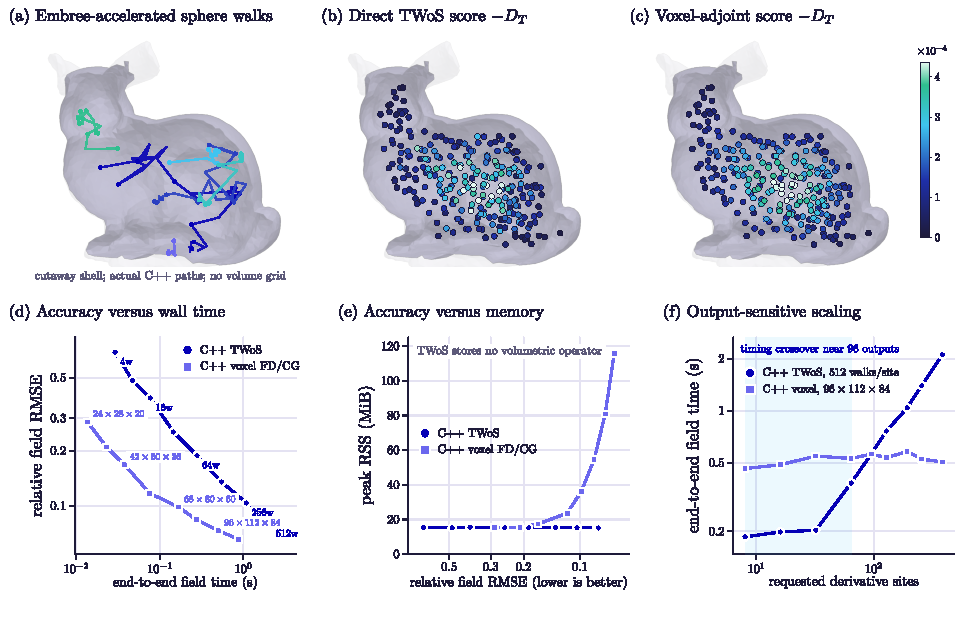
\includegraphics[width=\textwidth]{figures/compiled-bunny-scaling.pdf}
 \caption{Matched C++ scaling on the 69,674-triangle Bunny. (a) Actual
 Embree-accelerated sphere-walk trajectories in a shaded cutaway shell.
 (b--c) Direct TWoS and voxel topological scores at identical exposed interior
 sites and color scale. (d) Relative RMSE
 against an independent 2,048-walk field versus end-to-end time. (e) The same
 accuracy sweep versus measured process peak memory. (f) At nearly matched
 field error, the grid-free method is output-sensitive: the methods tie near
 96 requested sites, and the global voxel solve wins for dense output. Each point
 is measured rather than analytically extrapolated.}
 \label{fig:compiledbunny}
\end{figure}

At 64 outputs, TWoS takes $0.381$ seconds at relative RMSE $0.0622$;
the voxel reference takes $0.528$ seconds at RMSE $0.0711$.  Thus TWoS is
$1.39\times$ faster and its $15.4$ MiB peak is $5.25\times$ smaller than the
voxel process's $80.7$ MiB peak.  The speedup is $2.49\times$ at eight outputs
and the methods are effectively tied at 96 ($0.566$ versus $0.561$ seconds).
At 384 outputs the ordering reverses: TWoS
takes $2.10$ seconds and the voxel solve $0.504$ seconds.  This crossover is the
claimed performance result, not a universal speedup.  In the full-resolution
surface sweep, Embree BVH construction takes $9.74$ ms and the scalar closest-
boundary kernel sustains $1.77$ million queries per second.  Embree distances
agree with libigl to maximum absolute error $3.04\times10^{-7}$; the independent
C++ and Python TWoS fields correlate at $0.991$, and the C++ and SciPy voxel
fields agree to relative RMSE $1.11\times10^{-13}$ at the validation grid.

\paragraph{Independent high-sample check for the teaser.}
\label{app:renderprotocol}
For the 64-site comparison in \cref{fig:teaser}, we recomputed the reference
using an independent seed and 16,384 walks per site. Against this reference,
the retained TWoS and voxel score fields have relative RMSE $0.05888$ and
$0.06886$, respectively. The root-sum-square reference score standard error
divided by the reference score norm is $0.01160$, in addition to error from
the unchanged termination shell $\varepsilon=5\times10^{-4}$. This is a numerical accuracy check,
not exact ground truth; its timing is not included in the performance comparison.
The teaser separately visualizes fresh 256-walk temperature and insertion-benefit
estimates on a $160\times200$ section at $z=0.09$ for the saved cavity designs.
The physical domains do not contain the display opening. A one-grid-cell
Gaussian filter is applied only to the displayed scalar colors; raw fields,
accuracy errors, cooling objectives, and timing data are retained without it.
The placement study and sparse point-query timings are distinct experiments:
the latter does not establish a speedup for the displayed full design loop.

\subsection{Finned-housing design benchmark}

We next test the complete compiled design loop on a license-free stylized
engineering geometry rather than an animal scan.  An analytic union of a
rounded enclosure, nine heat-sink fins, and four mounting bosses is extracted
by marching cubes.  The resulting surface has 48,372 vertices and 96,740
triangles, is connected, closed, edge- and vertex-manifold, and has Euler
characteristic two.  This procedural construction is deliberately auditable;
it resembles a conduction housing but is not proprietary CAD.

Inside the housing we solve $-\Delta u=f$ with zero Dirichlet data on the outer
surface and every inserted cavity.  The positive source is a background plus
three anisotropic Gaussian hot spots representing two chips and a regulator;
the objective is the thermal compliance $J=\int_\Omega fu$.  On each WoS ball,
we sample its Green source integral with the unbiased beta-radial estimator in
\cref{prop:greenballsample}.  Each method inserts six radius-$0.095$ spherical
cavities from the same 768 Sobol candidates.  Sparse \method{} uses 12 scouting
walks per feasible candidate and 192 fresh walks on a 24-site shortlist; a
near-matched-time variant uses 96 and 768 walks, respectively.  Our strongest
deterministic baseline is a matrix-free geometric multigrid solver for the same
embedded seven-point operator, with four levels, three weighted-Jacobi pre- and
post-sweeps, residual-minimizing coarse correction, and relative residual
$10^{-6}$.  A predeclared sweep selects the smallest tested grid whose field
error is at most $0.09$, yielding $113\times73\times57$.  We also retain the
$96\times64\times54$ diagonal-preconditioned FD/CG baseline and random feasible
insertion.

All trajectory objectives use 384 fixed Sobol probes and 160 independent
walks per active probe.  We rerun each stochastic selector end to end for five
independent seeds; every final design is then evaluated with at least five fresh
384-walk streams, while the canonical and deterministic designs use ten.
Error bars for stochastic selectors are standard errors across complete design
runs; deterministic-baseline error bars isolate objective-evaluation noise.
Selection timings include BVH construction and every scouting/validation walk
for \method{}, or hierarchy construction, solve, and interpolation for
multigrid and FD/CG; all exclude process startup, file I/O, and the common
independent objective evaluation.



Across the five complete design runs, sparse and near-matched-time \method{}
reduce compliance by $68.90\%\pm0.84\%$ and $69.39\%\pm0.51\%$, respectively.
Tuned multigrid obtains $70.36\%\pm0.08\%$, FD/CG obtains
$69.96\%\pm0.10\%$, and five random designs obtain $27.76\%\pm4.57\%$.
Thus sparse \method{} realizes $97.9\%$ of the multigrid reduction in $0.432$
seconds rather than $1.861$ seconds, a $4.31\times$ speedup.  At near-matched
time, \method{} realizes $98.6\%$ of the multigrid reduction in $1.731$
seconds and uses $19.1$ MiB peak RSS rather than $31.4$ MiB, a $1.65\times$
memory reduction.  The near-matched-time mean is about one percentage point below multigrid.
The small seed count and the displayed standard errors do not establish
statistical equivalence; we report the quality--cost tradeoff directly.

Relative to a separate 512-walk TWoS field, the initial 128-walk \method{},
multigrid, and FD/CG fields have relative RMSE $0.163$, $0.0852$, and $0.0814$,
respectively.  The multigrid resolution sweep in
\cref{fig:housingtradeoffs}(a) therefore strengthens rather than weakens the
deterministic reference.  The design result does not claim that the inexpensive
scouting map is more accurate: shortlist validation recovers nearly all
multigrid design quality despite noisier global ranking.

\begin{figure}[t]
 \centering
 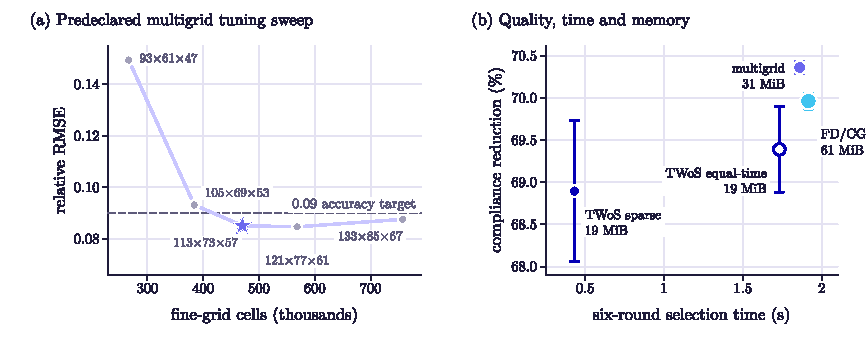
\includegraphics[width=0.89\textwidth]{figures/engineering-housing-tradeoffs.pdf}
 \caption{Tuning and resource tradeoff on the housing benchmark. (a) Five
 multigrid resolutions, each timed three times.  The star is the smallest grid
 meeting the predeclared relative-RMSE target $0.09$ against the independent
 512-walk field.  (b) Final design quality versus complete six-round selection
 time; marker area encodes peak memory and vertical bars show standard errors.
 Sparse \method{} occupies the fast regime, while the near-matched-time budget
 approaches the tuned multigrid solution without allocating a volume grid.}
\label{fig:housingtradeoffs}
\end{figure}

\subsection{Independent tetrahedral FEM audit}

We next remove implementation coupling from the initial-field comparison.  A
separate Python program uses scikit-fem 11.0.0~\cite{gustafsson2020scikitfem}
to assemble continuous piecewise-linear tetrahedra and SciPy's sparse direct
solver.  The only shared inputs are the analytic housing SDF, the analytic
load, and the CSV containing the 768 candidate coordinates; no C++ field,
grid, walk, or interpolation code is reused.  Background tetrahedra are kept
when their centroids lie inside the SDF, all exposed facets receive homogeneous
Dirichlet data, and the reported ranking density is $u_h^2$, since compliance
is self-adjoint for this load case.

We solve at $41\times27\times23$, $61\times39\times33$, and
$81\times51\times43$ background resolutions.  The finest retained mesh has
79,851 vertices and 393,616 tetrahedra; its free-DOF relative algebraic
residual is $5.45\times10^{-14}$.  End-to-end construction, assembly, solve,
and bounded-memory evaluation at all sites takes $20.37$ s and reaches 1.67 GiB
peak RSS in the untuned Python process.  The two coarser fields have relative
RMSE $0.1285$ and $0.0802$ against the finest field, respectively.

\begin{figure}[t]
 \centering
 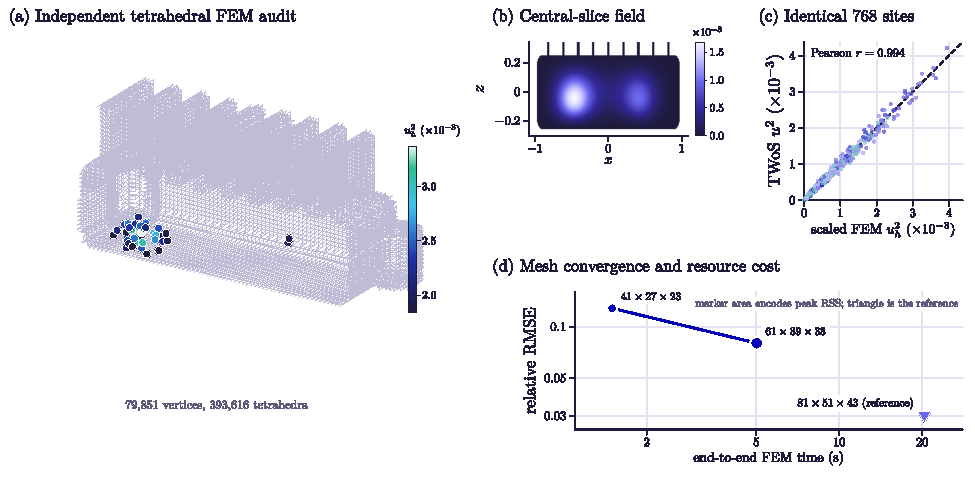
\includegraphics[width=0.92\textwidth]{figures/external-fem-audit.pdf}
 \caption{Independent external-solver field audit. (a) Cutaway boundary facets
 and high-ranking sites on the finest retained tetrahedral mesh. (b) Its
 central-slice $u_h^2$ field. (c) The independently assembled FEM density and
 512-walk TWoS score at the identical 768 candidates after one fitted positive
 scale; color encodes $x$ position. (d) End-to-end time and field convergence
 over three resolutions; marker area encodes measured peak RSS and the triangle
 denotes the finest reference.}
 \label{fig:externalaudit}
\end{figure}

Against the finest FEM field, 128-walk TWoS has Pearson correlation $0.9792$,
Spearman correlation $0.9849$, scale-fitted relative RMSE $0.1514$, and $80\%$
top-20 overlap.  At 512 walks these become $0.9943$, $0.9957$, $0.0789$, and
$95\%$, respectively; top-50 overlap is $92\%$.  The independent check also
supports the in-house reference: the $133\times85\times67$ multigrid field has
Pearson correlation $0.9989$, relative RMSE $0.0416$, and $95\%$ top-20
overlap against FEM.  This experiment validates the field and ranking across
discretization families.  It is not a claim that this centroid-classified mesh
is a production-quality body-fitted discretization, nor a comparison against a
complete level-set FEM optimizer.

\subsection{Connected cooling-channel growth and shape refinement}

The preceding comparison permits six disconnected cavities.  We next impose a
different, practically motivated topology: one connected channel must join two
separated terminals while removing the same nominal volume as the six
radius-$0.095$ spheres.  This constrained result is not compared as a quality
replacement for the unconstrained cavities; the latter remain an informative unconstrained reference, not a proved optimum or upper bound.

We score 3,072 interior Sobol candidates with 48-walk TWoS, select high-score
terminals on opposite sides of the housing, and construct a 24,365-edge
$k$-nearest-neighbor graph.  An edge's Euclidean length is multiplied by a
penalty for low endpoint topological score, and Dijkstra's algorithm supplies
the initial connection.  Resampling and safe smoothing give seven controls.
Fixed segment subdivisions produce a connected union of 22 overlapping balls,
as in \cref{eq:channelparameterization}.  A straight channel between the same
terminals is the geometry-only baseline.

The target removed volume is $0.0215482$.  Every connected trial radius is an
order-statistic calibration on the same $2^{20}$-point Sobol set; all three
reported channels attain QMC volume $0.0215479$, within one quantization bound
from \cref{prop:qmc-volume}.  At each shape round, 4,096 Differential WoS paths
per active probe estimate all 66 center coordinates jointly; the executable
also reports the 22 radius derivatives, hence 88 parameters.  With the explicit
safe-strip test, the six refinement passes take 3.62--3.82 seconds.  The normal
offset is $\ell=0.004$ and the one-offset-width admissible
patch is \cref{eq:channelsafepatch}.  We apply the exact transpose map
in \cref{eq:channelchainrule}, fix the endpoints, smooth the control proposal,
and project out first-order centerline-length change.  Each of the three step
scales uses eight fresh paired 320-walk objective streams.  A one-sided
Student-$t$ upper bound uses a predeclared Bonferroni allocation of $0.05$
across all 18 possible scale tests.  This follows the conditional protocol of
\cref{prop:fresh-shape} under a paired-normal interval assumption; exact
coverage is not established for the sampled differences.  Final values
use eight separate 768-walk streams.

\begin{figure}[t]
 \centering
 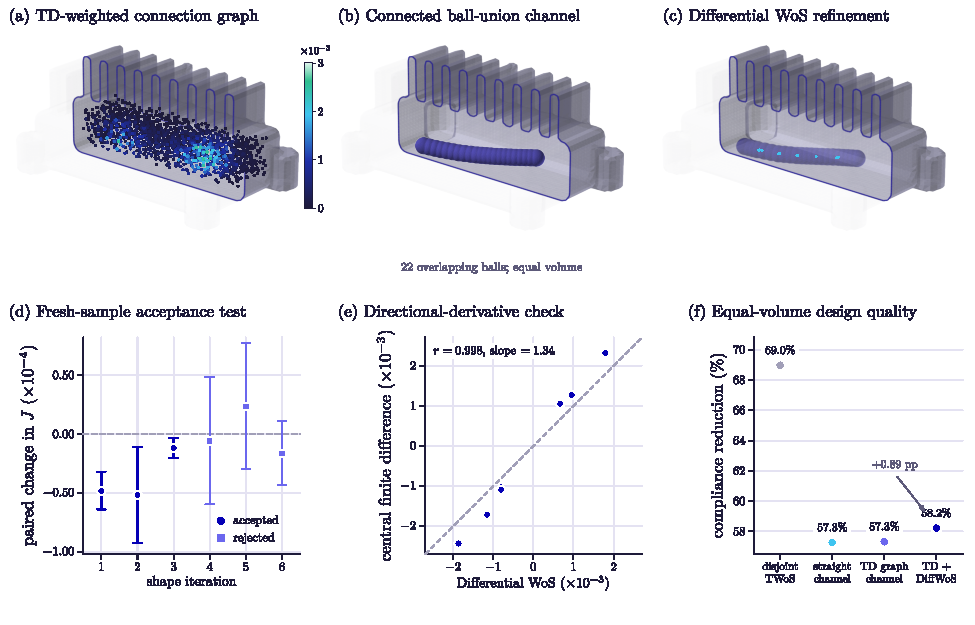
\includegraphics[width=\textwidth]{figures/engineering-housing-channels.pdf}
 \caption{From a topological field to a connected, refined cooling channel.
 (a) A TWoS field selects two terminals and weights the grid-free connection
 graph. (b) The shortest weighted path becomes a 22-ball connected channel.
 (c) Nested Differential WoS moves seven controls; the dashed centerline is
 the pre-refinement path. (d) Fresh paired line-search differences with
 Bonferroni-adjusted Student-$t$ whiskers under the paired-normal model; only a wholly negative interval is
 accepted. (e) Six independent high-signal tangent directions compare the
 fixed-radius Differential WoS derivative with central finite differences.
 (f) Independent final compliance reduction at matched nominal volume. The
 disconnected result is a topology-unconstrained reference, not a connected
 competitor.}
 \label{fig:housingchannels}
\end{figure}

The straight and topology-weighted graph channels reduce compliance by
$57.269\%\pm0.080\%$ and $57.325\%\pm0.048\%$, respectively; their paired
objective difference is not resolved ($-8.60\times10^{-6}\pm1.00\times10^{-5}$
SE).  With safe-strip truncation, the familywise procedure accepts the first
three Differential WoS steps and rejects the remaining tested updates.
Independent evaluation of the accepted shape gives $58.215\%\pm0.037\%$
reduction.  Relative to the unrefined graph channel, the objective decreases by
$2.086\%$; its paired absolute change is
$-1.356\times10^{-4}\pm8.00\times10^{-6}$ SE.  The unconstrained disconnected
design reaches $68.964\%\pm0.050\%$, showing a measured quality gap between these particular constructions; it does not establish the optimal cost of connectivity.

We audit the fixed-radius gradient at the pre-refinement graph channel with an
independent 8,192-walk Differential WoS pass and central differences of step
$0.012$, each using three paired 4,096-walk replicates.  To avoid a
noise-dominated correlation statistic, the predeclared seeded directions are
the descent direction plus five feasible tangent directions spanning the top
30\% of predicted signal; this audit therefore makes no claim about arbitrarily
weak directions.  Across the six signed directions, Pearson correlation is
$0.9982$, cosine similarity is $0.9982$, and the least-squares slope of finite
difference on Differential WoS is $1.341$.  The coherent scale difference is
consistent with finite-offset and finite-difference-step effects in
\cref{prop:channel-diffwos}; signs and relative magnitudes, which drive the
validated line search, agree closely.

\begin{figure}[t]
 \centering
 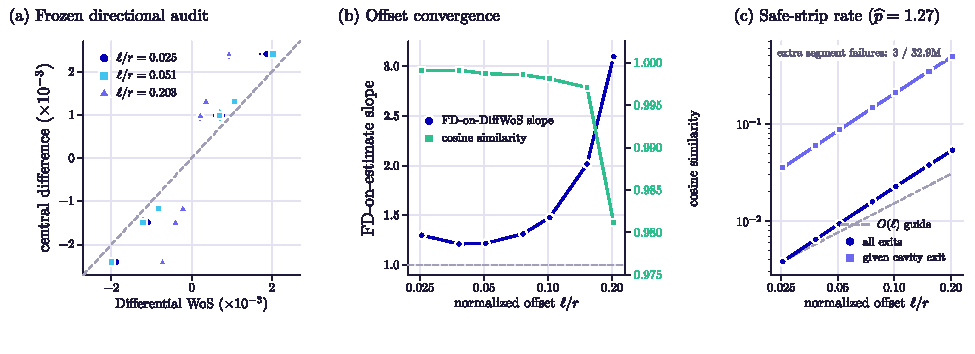
\includegraphics[width=\textwidth]{figures/offset-seam-sweep.pdf}
 \caption{Finite-offset and seam-strip audit on the frozen pre-refinement
 channel. (a) Central finite differences versus Differential WoS for six
 directions selected on a separate pilot stream, shown at the smallest,
 nominal, and largest offsets. (b) FD-on-Differential-WoS slope and cosine
 similarity across all seven normalized offsets. (c) The discarded harmonic
 exit mass, both over all exits and conditional on a cavity exit. The dashed
 line is an $O(\ell)$ reference, while $\widehat p$ is an unconstrained
 log--log fit. Error bars are standard errors over three independent streams;
 the random streams are matched across offsets.}
 \label{fig:offsetseamsweep}
\end{figure}

To isolate the normal offset, we freeze the same seven-control, 22-ball channel
and use an independent 8,192-walk pilot to select six feasible high-signal
length-tangent directions.  The reference central differences use three paired
4,096-walk replicates; each of seven offsets from $0.002$ to $0.016$ then uses
three independent 4,096-walk Differential WoS streams, with seeds matched
across offsets.  All six signs agree at every offset.  Through
$\ell/r=0.102$, cosine similarity is at least $0.9981$; at the deliberately
large $\ell/r=0.203$, it falls to $0.9811$ and the scale-corrected relative
$\ell_2$ error rises to $19.3\%$.  The smallest offset has greater
$1/\ell$ sampling noise: its FD-on-estimate slope is $1.303$, compared with
$1.216$ at $\ell=0.003$.  Linear extrapolation from offsets through $0.008$
has cosine $0.9993$ with the finite differences and FD-on-extrapolate slope
$1.167$; the residual scale difference also includes the finite FD step.

Across 32,858,112 outer paths, the discarded all-exit mass rises from
$0.003874\pm0.000048$ to $0.054123\pm0.000064$.  A log--log fit gives exponent
$1.269$ with $R^2=0.99991$; only three additional normal segments fail the
retained-domain check ($9.13\times10^{-8}$ of paths).  This is strong numerical
evidence for the geometric exit-mass component of
\cref{eq:weightedseamstrip} on this frozen configuration, but it neither
measures the $|\partial_nu|$ weight nor proves the asymptotic hypothesis.

The connected experiment demonstrates compatibility with existing-boundary refinement. Neither the topological graph initialization nor the measured line search supplies an unconditional certificate for the full geometry.

\subsection{Result summary}

\begin{table}[!htbp]
\centering
\caption{Measured results. Controlled diagnostics validate statistical mechanisms; the final rows report matched compiled comparisons, stochastic housing designs, and the equal-volume connected-channel refinement.}
\label{tab:controlledresults}
\begin{tabularx}{\textwidth}{@{}>{\raggedright\arraybackslash}p{0.2\textwidth}>{\raggedright\arraybackslash}p{0.17\textwidth}rr>{\raggedright\arraybackslash}X@{}}
\toprule
Experiment & Metric & Baseline & Ours & Outcome \\
\midrule
Smallest annulus capacity & Variance & $5.83\times10^{-3}$ & $7.06\times10^{-4}$ & $8.26\times$ below coupled finite cavity \\
Correlation $0.9$ & Absolute bias & $2.708\times10^{-1}$ & $7.50\times10^{-4}$ & same-seed error floor removed \\
256 null candidates & False insertion & $100.0\%$ & $5.003\%$ & fresh validation meets 5\% target \\
6,359-site WoS field & Spatial RMSE & $0.1078$ & $0.0196$ & $5.50\times$ below same-seed product \\
64-site C++ field & Wall time (s) & $0.528$ & $0.381$ & $1.39\times$ faster than voxel FD/CG \\
384-site, $\approx0.075$ RMSE & Peak RSS (MiB) & $80.6$ & $15.6$ & $5.17\times$ smaller than voxel FD/CG \\
Housing, sparse budget & Compliance reduction & $70.36\%$ & $68.90\%$ & $97.9\%$ of tuned multigrid reduction \\
Housing, sparse budget & Wall time (s) & $1.861$ & $0.432$ & $4.31\times$ faster than tuned multigrid \\
Housing, near-matched time & Compliance reduction & $70.36\%$ & $69.39\%$ & $98.6\%$ of tuned multigrid reduction \\
Housing, near-matched time & Peak RSS (MiB) & $31.4$ & $19.1$ & $1.65\times$ smaller than tuned multigrid \\
External FEM field audit & Pearson correlation & $1.000$ & $0.9943$ & 512-walk TWoS on identical 768 sites \\
External FEM field audit & Top-20 agreement & $100\%$ & $95\%$ & cross-discretization ranking agreement \\
Connected housing channel & Compliance reduction & $57.325\%$ & $58.215\%$ & $2.086\%$ lower objective after safe-strip DiffWoS refinement \\
Channel derivative audit & Pearson correlation & --- & $0.9982$ & six high-signal tangent directions \\
Channel offset audit & Discarded-mass exponent & $O(\ell)$ reference & $1.269$ & $R^2=0.99991$ over 32.86M paths \\
\bottomrule
\end{tabularx}
\end{table}


\FloatBarrier
\section{Accelerated Sampling and Baseline Components}
\label{sec:critical}
% Generated from retained raw experiments; do not edit.
\newcommand{\SourceArrayMSE}{2.51\times10^{-8}}
\newcommand{\SourceMCMSE}{5.00\times10^{-7}}
\newcommand{\SourceRatio}{19.9}
\newcommand{\SourceArrayTime}{1.008}
\newcommand{\SourceMCTime}{0.073}
\newcommand{\NeighborRatio}{1.96}
\newcommand{\ShapeInitial}{1.35\times10^{-3}}
\newcommand{\ShapeMinimum}{1.41\times10^{-8}}
\newcommand{\ShapeMaximum}{9.39\times10^{-8}}
\newcommand{\SealedEigen}{2.24\times10^{-5}}


\begin{figure}[t]
 \centering
 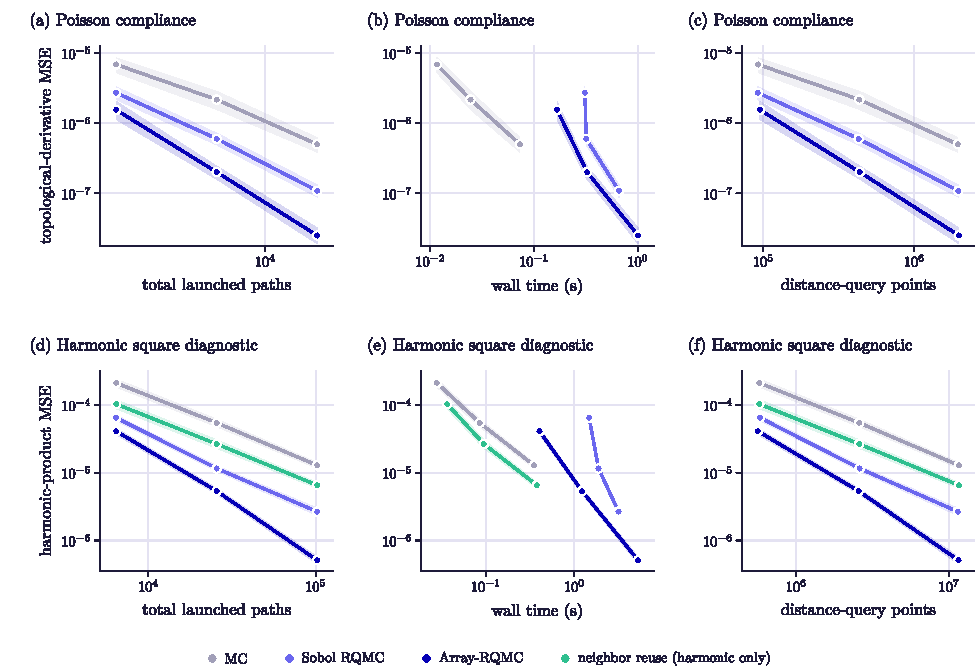
\includegraphics[width=0.975\textwidth]{figures/accelerated-sampling.pdf}
 \caption{Measured accelerated sampling with independent-batch cross-fitting.
 Top: the actual Poisson-compliance topological derivative on the disk.
 Bottom: a manufactured harmonic-product diagnostic on the square, including
 neighbor reuse.  All methods have equal launched-path budgets at corresponding
 markers.  The three columns expose the difference between statistical
 efficiency, Python wall time, and distance-query cost.  Bands describe
 uncertainty in empirical MSE across 32 independent full runs.}
 \label{fig:accelerated}
\end{figure}

\paragraph{A genuine Poisson-compliance derivative.}
On the unit disk, solve $-\Delta u=1$ with homogeneous Dirichlet data and
$J=\int_\Omega u$.  Then $p=u=(1-|z|^2)/4$ and
$D_T(z)=-(1-|z|^2)^2/16$.  Each WoS ball contributes the exact
constant-source Green integral $r^2/4$, with the same implementation for MC,
scrambled-Sobol RQMC, and shifted-Korobov Array-RQMC~\cite{ho2026array}.
We use five fixed sites, four independently randomized batches, 64, 256,
or 1,024 paths per batch, and 32 complete replications at each setting.
All products are cross-fitted across batches, as required by
\cref{app:batchindependence}; trajectories inside an array are never treated
as independent samples.  The shell tolerance is $10^{-7}$, and exhaustion of
the 256-step cap raises an error.  The maximum marginal truncation bias is
$\varepsilon/2$ here; it is not silently equated with zero.

At 1,024 paths per batch, Array-RQMC has mean TD MSE
$\SourceArrayMSE$ versus $\SourceMCMSE$ for MC, a
$\SourceRatio\times$ reduction at equal launched-path budget.
The corresponding median times are $\SourceArrayTime$ s and
$\SourceMCTime$ s.  Thus the measured Python implementation trades lower
error per path for substantial sorting overhead.  It establishes no uniform
runtime advantage.  RNG initialization and distance queries are included;
the timing applies only to these implementations and scenes.
The final Poisson campaign runs without other benchmark jobs; harmonic
timings come from a shared runtime and are exploratory.
\Cref{fig:accelerated} reports error against paths, time, and query count;
bands are percentile bootstrap intervals for mean MSE across the 32 full
replications, not certified insertion intervals.

\paragraph{Neighbor reuse on harmonic diagnostics.}
On both disk and square, we reuse the manufactured harmonic polynomials from
the earlier field diagnostic at 25 fixed sites in $[-0.55,0.55]^2$.
These nonzero-boundary harmonic pairs test the product-estimator algebra;
they are not the state and homogeneous-boundary adjoint of the Poisson
compliance problem above.  We implement the deterministic variance-bound
weights in Czekanski et al.~\cite{czekanski2026neighbors}, equations (17)--(18),
and retain the first sphere exit and final boundary value of every walk.
Both queries and weights are computed inside each independent batch.
At the largest square budget, neighbor reuse reduces product MSE by
$\NeighborRatio\times$ relative to MC using the same launched paths.
Our 13-bit Hilbert implementation matches the authors' Array-RQMC update
routine in four common-randomization cases to within $10^{-12}$.
We do not apply terminal-only neighbor reweighting to a source PDE:
its first-ball source contribution would need a separate correct treatment.

\begin{figure}[t]
 \centering
 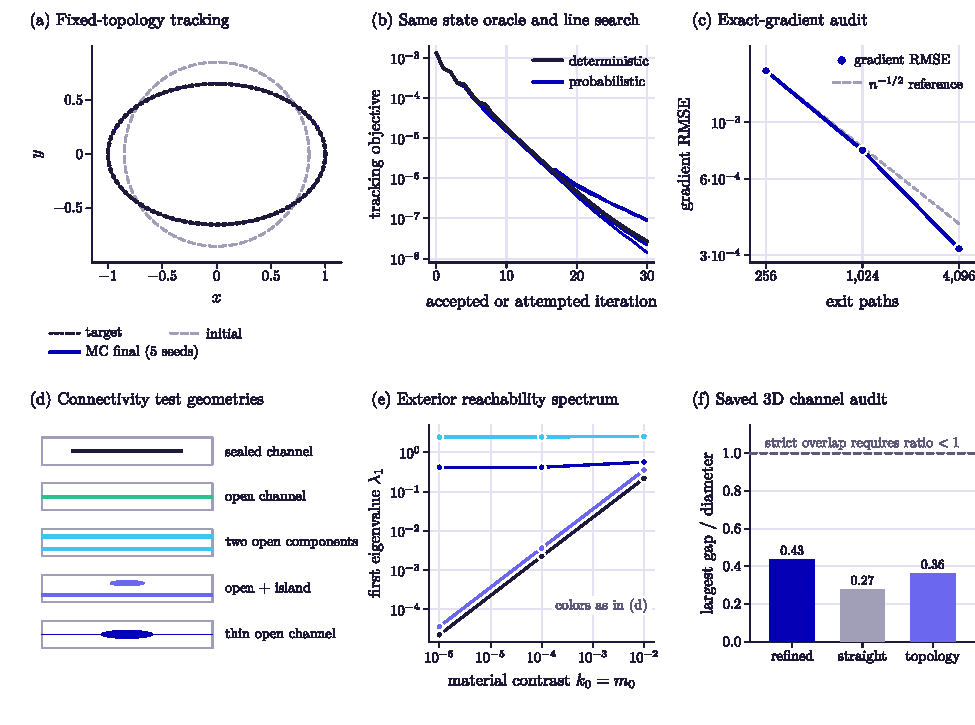
\includegraphics[width=0.985\textwidth]{figures/baseline-diagnostics.pdf}
 \caption{Baseline components and geometric feasibility.  (a--c) Exact-state
 ellipse tracking tests the probabilistic shape derivative and descent, with
 five stochastic runs.  (d--e) The reproduced two-phase spectral operator
 distinguishes sealed islands from exterior-connected voids; two open
 components are allowed.  (f) Existing 3D ball-chain designs satisfy the newly
 explicit strict-overlap guard.  These are component experiments, not complete
 PINN/FEM or level-set optimizer reproductions.}
 \label{fig:baselinecomponents}
\end{figure}

\paragraph{Fixed-topology probabilistic shape control.}
We specialize a probabilistic derivative~\cite{schmidt2026first}
to a two-parameter ellipse family, giving both optimizers the same exact
Poisson state.  The target has semiaxes $(1,0.65)$; the initial semiaxes are
$(0.85,0.85)$.  We compare the uniform-start, importance-weighted exit formula
with a separately derived deterministic pullback gradient
(\cref{app:shapeoracle}).  The deterministic gradient agrees with central
differences to within $10^{-8}$; 48 replications at each of three path budgets
audit the stochastic error.  With identical bounds and Armijo line searches,
five stochastic 30-step runs reduce the tracking objective from
$\ShapeInitial$ to the range $[\ShapeMinimum,\ShapeMaximum]$.
This validates the shape-derivative implementation on a fixed-topology design
task.  It does not measure neural-state training, boundary FEM smoothing,
or the complete published optimizer, and does not compare full optimizers.

\paragraph{Spectral connectivity reproduction and geometry correction.}
We reproduce the two-phase Dirichlet eigenproblem of
Andrade et al.~\cite{andrade2026connectivity}, equation (4), with $P_1$
triangles and consistent mass.  The cavity coefficients are $k_1=m_1=1$;
the other phase has $k_0=m_0\in\{10^{-2},10^{-4},10^{-6}\}$.
Five geometries and three mesh resolutions produce 45 eigenproblem solves.
At the finest $129\times129$ node resolution and contrast $10^{-6}$,
the sealed connected strip has $\lambda_1\approx\SealedEigen$, while
one open strip and two disconnected open strips both have
$\lambda_1\approx2.47$.  The latter is close to the limiting mixed-boundary
value $\pi^2/4$.  Thus their constraint tests exterior reachability, which is
different from connectedness of our interior channel.  At nonzero contrast,
even an isolated cavity has a positive eigenvalue; a threshold needs its own
contrast and resolution study.

After each radius recalibration, consecutive balls must overlap strictly. All three retained designs satisfy this check, with maximum gap/diameter ratios from $0.275$ to $0.434$. The geometric guarantee and its exterior-access limitation are proved in \cref{app:ballchain}.
\Cref{fig:baselinecomponents} separates these validation results from the
complete application comparisons, which were not performed for these two external methods.


\end{document}
